\documentclass[runningheads]{llncs}

\usepackage[T1]{fontenc}
\usepackage{graphicx}
\usepackage{amsmath,amssymb}
\usepackage{booktabs}
\usepackage{makecell}
\usepackage{multirow}
\usepackage{array}
\usepackage{subcaption}
\usepackage[hyphens]{url}
\usepackage{hyperref}
\usepackage{tikz}
\usetikzlibrary{shapes.geometric,arrows.meta,positioning,calc,fit,backgrounds}

\hypersetup{
    colorlinks=true,
    linkcolor=blue,
    filecolor=magenta,      
    urlcolor=cyan,
    citecolor=blue,
}

\graphicspath{{./images/}}
\setlength\tabcolsep{6pt}
\raggedbottom

\begin{document}

\title{SkelGym: Cross-Paradigm Kinematic Fusion and Geometry-Preserving Skeletal Augmentation for 22-Class Gym Exercise Classification}

\titlerunning{SkelGym: Cross-Paradigm Kinematic Fusion}

\author{Xuan-Cuong Nguyen\inst{1}\orcidID{0000-0002-1825-0097} \and
Nhat-Quang Truong\inst{1}\thanks{Corresponding author.}\orcidID{0009-0005-4321-8765} \and
Quoc-Trinh Vo\inst{1}}

\authorrunning{X.-C. Nguyen et al.}

\institute{FPT University, FPT City, Ngu Hanh Son, Da Nang 550000, Viet Nam\\
\email{cuongnxde180528@fpt.edu.vn}, \email{quangtnde180544@fpt.edu.vn}
}

\maketitle

\begin{abstract}
Automated gym exercise recognition is critical for developing intelligent virtual personal trainer systems capable of monitoring workout execution, tracking training volume, and mitigating musculoskeletal injury risks. However, traditional RGB video approaches incur prohibitive computational costs, suffer from environmental background overfitting, and raise severe privacy concerns when streaming from home environments. We evaluate on a curated corpus of 1,024 in-the-wild videos spanning 22 fine-grained resistance exercises under strict video-level partitioning with no source-video overlap across train, validation, and test sets. We present \textbf{SkelGym}, a lightweight, privacy-aware intelligent exercise recognition framework operating exclusively on 3D skeletal coordinates extracted via monocular pose estimation. SkelGym introduces four primary technical contributions: (1) a curated, multi-source 3D skeletal benchmark spanning 1,024 videos across 22 resistance exercises under strict video-level partitioning with zero source-video overlap across train, validation, and test sets; (2) a 63-dimensional \textit{Biomechanical Compound Representation} (Biomechanical Mix v2) fusing pelvic-centered metric World 3D coordinates (39-d) with domain-selected kinematic angles (24-d) via dual-branch projection; (3) \textit{SkelGym-Aug}, an empirically selected, task-oriented augmentation configuration restricted to distance-preserving Euclidean transformations (sagittal bilateral reflection and gravitational yaw rotation) selected strictly on validation-window evidence; and (4) a cross-paradigm ensemble coupling a self-attention Transformer with a four-stream Adaptive Graph Convolutional Network via zero-parameter uniform average soft voting (SkelGym-Full) and validation-calibrated accuracy-weighted soft voting (SkelGym-Lite), achieving real-time low-latency edge classification. Evaluated across three independent random seeds under fixed splits ($N=2,743$ test windows from 233 held-out videos), SkelGym achieves \textbf{76.19\% $\pm$ 0.16\% window-level accuracy} (Window Macro F1: \textbf{0.7537 $\pm$ 0.0014}) and \textbf{85.27\% $\pm$ 0.41\% video-level consensus accuracy} (Video Macro F1: \textbf{0.8386 $\pm$ 0.0075}, with 200 of 233 held-out videos correctly classified, achieving 85.84\% accuracy on the canonical test run). All pairwise architectural transitions are verified via paired statistical hypothesis testing (window-level McNemar $p \le 5.88 \times 10^{-5}$ across all transitions; video-level posterior confidence differences confirmed across sequence-to-ensemble transitions). With an ultra-low classifier inference latency of merely \textbf{0.49--3.96~ms} on host CPU (0.59--4.65~ms on CUDA, where individual backbones execute in 0.49--1.03~ms and the full five-stream ensemble executes in 3.96~ms at 253 FPS) per 32-frame window, SkelGym enables real-time, privacy-aware exercise recognition suitable for smart mirrors, mobile devices, and embedded gym displays. All source code, extracted skeletal representations, metadata, and pretrained checkpoints used for reproducibility are publicly available at \url{https://huggingface.co/Cuong2004/gym-exercise-classification}.

\keywords{Gym exercise classification \and Skeleton-based action recognition \and Adaptive Graph Convolutional Networks \and Skeletal Transformers \and Biomechanical features \and Real-time inference \and Edge AI.}
\end{abstract}


\section{Introduction}

Regular physical resistance training and structured exercise play an essential role in improving cardiovascular health, metabolic longevity, muscular hypertrophy, and psychological well-being \cite{schoenfeld2010}. With modern demanding lifestyles and remote working environments, a rapidly growing population conducts workouts in home settings rather than commercial fitness centers. However, exercising without the supervision of certified strength and conditioning coaches frequently leads to improper kinetic execution, sub-optimal muscular recruitment, and elevated risks of acute or repetitive strain injuries (such as lumbar disc herniation, rotator cuff impingement, and patellar tendinopathy) \cite{riccio2024}. Consequently, there is an urgent demand for automated, intelligent virtual personal trainers capable of identifying exercise types in real-time, monitoring execution repetitions, and providing instantaneous biomechanical feedback \cite{garciadevilla2022}.

Early computer vision frameworks for resistance exercise and action recognition were predominantly built upon appearance-based RGB video models, such as 2D/3D CNNs \cite{donahue2015,carreira2017,feichtenhofer2019} and spatiotemporal Vision Transformers (e.g., ViViT \cite{arnab2021}, TimeSformer \cite{bertasius2021}, Video Swin \cite{liu2022video}). While dense RGB representations capture visual cues such as gym equipment and barbells \cite{ng2015}, they exhibit three critical operational drawbacks in practical deployments.

First, dense spatio-temporal convolutions incur heavy computational overhead (often exceeding hundreds of GFLOPs), which precludes real-time execution on resource-constrained mobile phones, smart displays, or edge hardware. Second, appearance-based networks readily memorize spurious background correlations---including flooring patterns, studio lighting, bench upholstery, and athletic apparel---resulting in severe performance collapse when evaluated in novel domestic workout environments. Third, cloud-centric video architectures necessitate continuously transmitting unconstrained high-definition RGB video streams from private living spaces to remote servers, introducing network bandwidth bottlenecks and user privacy vulnerabilities.

\begin{figure*}[!t]
\centering
\resizebox{\textwidth}{!}{
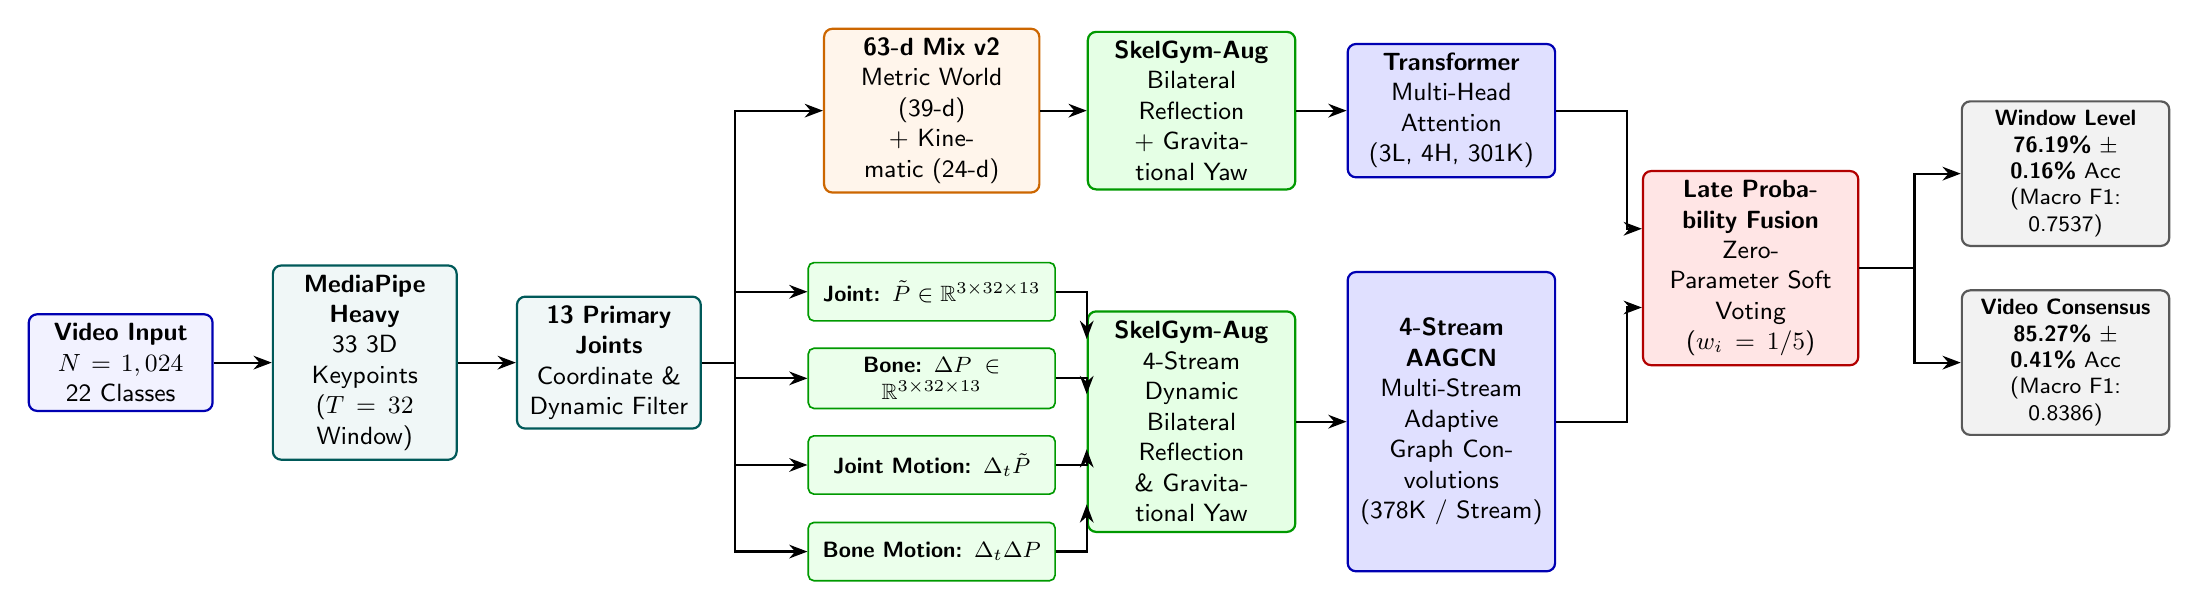
\begin{tikzpicture}[
    font=\sffamily\small,
    >=Stealth,
    block/.style={rectangle, draw=blue!70!black, fill=blue!5, rounded corners=3pt, text width=2.1cm, minimum height=1.15cm, align=center, line width=0.8pt},
    proc/.style={rectangle, draw=teal!70!black, fill=teal!6, rounded corners=3pt, text width=2.1cm, minimum height=1.15cm, align=center, line width=0.8pt},
    stream/.style={rectangle, draw=green!60!black, fill=green!8, rounded corners=2pt, text width=2.9cm, minimum height=0.74cm, align=center, line width=0.6pt, font=\sffamily\footnotesize},
    seqbox/.style={rectangle, draw=orange!80!black, fill=orange!8, rounded corners=3pt, text width=2.5cm, minimum height=1.25cm, align=center, line width=0.8pt},
    model/.style={rectangle, draw=blue!70!black, fill=blue!12, rounded corners=3pt, text width=2.4cm, minimum height=1.35cm, align=center, line width=0.8pt},
    modelaagcn/.style={rectangle, draw=blue!70!black, fill=blue!12, rounded corners=3pt, text width=2.4cm, minimum height=3.8cm, align=center, line width=0.8pt},
    augbox/.style={rectangle, draw=green!60!black, fill=green!10, rounded corners=3pt, text width=2.4cm, minimum height=1.25cm, align=center, line width=0.8pt},
    augboxaagcn/.style={rectangle, draw=green!60!black, fill=green!10, rounded corners=3pt, text width=2.4cm, minimum height=2.8cm, align=center, line width=0.8pt},
    fusion/.style={rectangle, draw=red!70!black, fill=red!10, rounded corners=3pt, text width=2.5cm, minimum height=1.7cm, align=center, line width=0.8pt},
    output/.style={rectangle, draw=gray!70!black, fill=gray!10, rounded corners=3pt, text width=2.4cm, minimum height=1.15cm, align=center, line width=0.8pt, font=\sffamily\footnotesize}
]

% Input & Feature Extraction (y = 0)
\node[block] (input) at (0, 0) {\textbf{Video Input}\\ $N=1,024$\\ 22 Classes};
\node[proc] (mp) at (3.1, 0) {\textbf{MediaPipe Heavy}\\ 33 3D Keypoints\\ ($T=32$ Window)};
\node[proc] (filter) at (6.2, 0) {\textbf{13 Primary Joints}\\ Coordinate \&\\ Dynamic Filter};

% Top Branch: Transformer Mix (y = 3.2, generous vertical clearance)
\node[seqbox] (comp) at (10.3, 3.2) {\textbf{63-d Mix v2}\\ Metric World (39-d)\\ + Kinematic (24-d)};
\node[augbox] (aug1) at (13.6, 3.2) {\textbf{SkelGym-Aug}\\ Bilateral Reflection\\ + Gravitational Yaw};
\node[model] (trans) at (16.9, 3.2) {\textbf{Transformer}\\ Multi-Head Attention\\ (3L, 4H, 301K)};

% Bottom Branch: Multi-Stream AAGCN (y = 0.9 to -2.4, generous vertical clearance)
\node[stream] (joint) at (10.3, 0.9) {\textbf{Joint:} $\tilde{P} \in \mathbb{R}^{3 \times 32 \times 13}$};
\node[stream] (bone)  at (10.3, -0.2) {\textbf{Bone:} $\Delta P \in \mathbb{R}^{3 \times 32 \times 13}$};
\node[stream] (jmot)  at (10.3, -1.3) {\textbf{Joint Motion:} $\Delta_t \tilde{P}$};
\node[stream] (bmot)  at (10.3, -2.4) {\textbf{Bone Motion:} $\Delta_t \Delta P$};

\node[augboxaagcn] (aug2) at (13.6, -0.75) {\textbf{SkelGym-Aug}\\ 4-Stream Dynamic\\ Bilateral Reflection\\ \& Gravitational Yaw};

\node[modelaagcn] (aagcn) at (16.9, -0.75) {\textbf{4-Stream AAGCN}\\ Multi-Stream Adaptive\\ Graph Convolutions\\ (378K / Stream)};

% Fusion & Outputs
\node[fusion] (softvote) at (20.7, 1.2) {\textbf{Late Probability Fusion}\\ Zero-Parameter Soft\\ Voting ($w_i = 1/5$)};

\node[output] (out_win) at (24.7, 2.4) {\textbf{Window Level}\\ \textbf{76.19\% $\pm$ 0.16\%} Acc\\ (Macro F1: 0.7537)};
\node[output] (out_vid) at (24.7, 0.0) {\textbf{Video Consensus}\\ \textbf{85.27\% $\pm$ 0.41\%} Acc\\ (Macro F1: 0.8386)};

% Arrows: Stage 1
\draw[->, thick] (input) -- (mp);
\draw[->, thick] (mp) -- (filter);

% Distribution Bus from filter to parallel tracks
\draw[thick] (filter.east) -- (7.8, 0) coordinate (trunk);
\draw[->, thick] (trunk) |- (comp.west);
\draw[->, thick] (trunk) |- (joint.west);
\draw[->, thick] (trunk) |- (bone.west);
\draw[->, thick] (trunk) |- (jmot.west);
\draw[->, thick] (trunk) |- (bmot.west);

% Connections: Upper Track
\draw[->, thick] (comp) -- (aug1);
\draw[->, thick] (aug1) -- (trans);

% Connections: Lower Track (individual dedicated channels into aug2)
\draw[->, thick] (joint.east) -| ($(aug2.west)+(0, 1.05)$);
\draw[->, thick] (bone.east)  -| ($(aug2.west)+(0, 0.35)$);
\draw[->, thick] (jmot.east)  -| ($(aug2.west)-(0, 0.35)$);
\draw[->, thick] (bmot.east)  -| ($(aug2.west)-(0, 1.05)$);

\draw[->, thick] (aug2) -- (aagcn);

% Connections into Fusion
\draw[->, thick] (trans.east) -- ++(0.9, 0) |- ($(softvote.west)+(0, 0.5)$);
\draw[->, thick] (aagcn.east) -- ++(0.9, 0) |- ($(softvote.west)-(0, 0.5)$);

% Output arrows
\draw[->, thick] (softvote.east) -- ++(0.7, 0) |- (out_win.west);
\draw[->, thick] (softvote.east) -- ++(0.7, 0) |- (out_vid.west);

\end{tikzpicture}
}
\caption{The proposed SkelGym architecture: an end-to-end cross-paradigm framework coupling self-attention sequence modeling with multi-stream adaptive graph convolutional networks via zero-parameter uniform average soft voting.}
\label{fig:pipeline_full}
\end{figure*}

Skeleton-based human action recognition offers an elegant solution to these challenges by abstracting human bodily movement into sparse, lightweight 3D keypoint coordinates. With real-time pose estimation frameworks such as Google MediaPipe \cite{chuankun2019,bazarevsky2020}, OpenPose \cite{cao2019}, and AlphaPose \cite{fang2022}, 3D skeletal tracking can be executed on commodity webcams and mobile chipsets at sub-millisecond latencies. However, translating skeletal tracking into accurate, multi-class gym exercise recognition introduces four fundamental scientific hurdles:

The first hurdle is the scarcity of standardized, fine-grained 3D skeletal gym benchmarks with strict source-video partitioning. Existing fitness datasets are either restricted to trivial 3--5 exercises or employ random temporal window splits that permit subtle data leakage between training and testing partitions, while also lacking multi-source in-the-wild recording diversity.

The second hurdle concerns biomechanical redundancy versus kinematic expressiveness. Resistance exercises frequently involve fine-grained differences in limb trajectories and joint angles, as demonstrated when distinguishing flat, incline, and decline bench presses, or differentiating conventional deadlifts from Romanian deadlifts. While exhaustive geometric angle formulations---such as computing all three-joint triplets---might capture these subtle distinctions, they incur a combinatorial explosion of features ($\binom{13}{3} = 286$), introducing dimensional multicollinearity, gradient singularities at joint lockouts, and an acute risk of overfitting.

The third hurdle stems from the lack of task-oriented validation for skeletal data augmentation. While spatial and temporal transformations (such as rotation, mirroring, scaling, time warping, and jitter) are well-established in general action recognition, applying them naively to resistance training risks altering fixed anatomical bone lengths, violating gravitational verticality, or distorting repetition cadence and velocity profiles that define distinct exercise classes.

Finally, the fourth hurdle lies in achieving true cross-paradigm model complementarity and real-time edge execution while strictly preventing data contamination. Temporal sequence architectures (such as LSTMs \cite{hochreiter1997long,graves2005} and Transformers \cite{vaswani2017}) excel at modeling long-range phase transitions, whereas spatial-temporal graph convolutional networks (such as ST-GCN \cite{yan2018}, 2S-AGCN \cite{shi2019two}, and CTR-GCN \cite{chen2021channel}) explicitly exploit physical musculoskeletal topology. Prior works often combine these paradigms naively, rely on heavy pre-trained backbones unsuitable for edge hardware, or tune ensemble fusion weights directly on test partitions, inducing optimistic reporting bias.

To systematically resolve these challenges, we introduce \textbf{SkelGym} (illustrated in Fig.~\ref{fig:pipeline_full}), an end-to-end intelligent exercise recognition system that transforms raw monocular video into actionable exercise labels through a fully automated pipeline: \textit{Video $\rightarrow$ MediaPipe 3D Skeleton $\rightarrow$ 63-d Biomechanical Representation $\rightarrow$ SkelGym-Aug $\rightarrow$ Cross-Paradigm Classifiers $\rightarrow$ Late Probability Fusion $\rightarrow$ Video Consensus $\rightarrow$ Edge Deployment}. Specifically, this work provides four primary technical contributions:

\paragraph{C1: Multi-Source 3D Skeletal Landmark Benchmark with Leakage-Free Partitioning.} We curate and release a fine-grained 3D skeletal dataset derived from 1,024 multi-camera in-the-wild videos spanning 22 resistance training exercises across three provenance streams (public repositories, stock media, and 128 ethical author-recorded gymnasium videos). Pre-extracted into 13 load-bearing 3D landmark trajectories (1,108 action segments) in JSON, NPY, and HDF5 formats under CC~BY~4.0 and MIT licenses, our benchmark establishes a strict video-level partitioning protocol (6:2:2) with zero source-video overlap, completely eliminating temporal window-level data leakage: no frames, windows, or action segments from the same source video cross partition boundaries.

\paragraph{C2: Biomechanical Compound Representation (63-d Mix v2).} We design an upgraded kinematic descriptor fusing metric World 3D coordinates (39-d) with 24-d kinematic joint articulation and limb elevation angles. Spatial coordinates are expressed in estimated physical metric dimensions (meters) centered at the pelvic mid-hip origin anchor. The angular branch distills 24 anatomically calibrated angles (14 limb segment orientation angles relative to gravity and 10 3D joint articulation triplets), resolving collinearity and gradient singularities while providing intrinsic invariance to horizontal camera yaw rotation.

\paragraph{C3: Empirically Selected Task-Oriented Augmentation Configuration (SkelGym-Aug).} Rather than claiming novel mathematical transformation operators, we evaluate a candidate pool of established skeletal augmentations categorized into geometric (sagittal reflection, gravitational yaw rotation, proportional scaling), temporal (time warping), and noise-based (sensor jitter) domains. Through systematic Leave-One-Out (LOO) and isolated ablations evaluated strictly on validation-window metrics across three independent random seeds, we demonstrate that unconstrained scaling and jitter distort physical metric proportions and velocity profiles, while temporal time warping disrupts exercise tempo and cadence. We thus isolate an optimal, task-oriented 2-operator configuration---Bilateral Sagittal Reflection and Gravitational Yaw Rotation ($\pm 15^\circ$)---that strictly preserves physical Euclidean distances and gravitational verticality, achieving peak representation learning (Validation Window Accuracy: 81.20\% $\pm$ 0.72\%, Macro F1: 0.8119 $\pm$ 0.0072) with zero test-time data corruption.

\paragraph{C4: Cross-Paradigm Fusion, Rigorous Benchmarking, and Real-Time Edge Deployment.} We engineer custom lightweight backbones ($\approx 301\text{K}$--$378\text{K}$ parameters each, trained entirely from scratch) spanning self-attention sequence Transformers and four-stream Adaptive Graph Convolutional Networks (AAGCN), unified via transparent late probability fusion: zero-parameter uniform average soft voting for the full cross-paradigm ensemble (SkelGym-Full) and validation-calibrated accuracy-weighted soft voting for the two-stream edge variant (SkelGym-Lite). Through multi-seed evaluations across three independent random seeds ($42, 123, 3407$) and paired statistical hypothesis testing (window-level McNemar $p \le 5.88 \times 10^{-5}$ across all transitions; video-level posterior confidence differences confirmed across sequence-to-ensemble transitions), SkelGym attains \textbf{76.19\% $\pm$ 0.16\% window accuracy} (Window Macro F1: \textbf{0.7537 $\pm$ 0.0014}) and \textbf{85.27\% $\pm$ 0.41\% video consensus accuracy} (Video Macro F1: \textbf{0.8386 $\pm$ 0.0075}, correctly classifying 200 of 233 held-out test videos) across 22 resistance exercises. Delivering an ultra-low single-window classifier latency of merely \textbf{0.49--3.96~ms} on host CPU (0.59--4.65~ms on CUDA, where individual backbones execute in 0.49--1.03~ms and the full 5-stream ensemble executes in 3.96~ms at 253 FPS), SkelGym demonstrates practical real-time feasibility for privacy-aware edge deployment without persistent video streaming.

\section{Related Work}

\subsection{Skeletal Action Recognition}
Extracting human pose from monocular RGB video has matured rapidly with lightweight real-time estimators such as OpenPose \cite{cao2019}, AlphaPose \cite{fang2022}, and Google MediaPipe Pose \cite{chuankun2019,bazarevsky2020}. Early landmark-based action recognition utilized Recurrent Neural Networks (RNNs) and Long Short-Term Memory (LSTM) networks \cite{hochreiter1997long,graves2005,li2017} to model skeletal temporal dynamics. However, pure recurrent models treat skeletons as unorganized coordinate vectors, ignoring the inherent topological structure of the human musculoskeletal system.

To overcome this, Yan et al. \cite{yan2018} pioneered Spatial Temporal Graph Convolutional Networks (ST-GCN), constructing a spatio-temporal graph where human joints form vertices and physical bones form fixed spatial edges. Shi et al. \cite{shi2019two} introduced Two-Stream Adaptive Graph Convolutional Networks (2S-AGCN), parameterizing the adjacency matrix with learnable and data-driven components. Subsequent advances---including multi-stream AAGCN \cite{shi2020skeleton}, CTR-GCN \cite{chen2021channel}, InfoGCN \cite{chi2022infogcn}, HD-GCN \cite{lee2023hdgcn}, and SkateFormer \cite{zheng2024skateformer}---progressively integrated channel attention, information-theoretic representation learning, hierarchical graph decomposition, and partition-specific transformer attention. In parallel, Duan et al. \cite{duan2022} introduced PoseConv3D, mapping 3D skeleton keypoints to spatiotemporal heatmap volumes to exploit 3D convolutional architectures, while Yin et al. \cite{yin2023} designed an efficient multi-stream depthwise separable convolutional network for skeleton action recognition. However, these modern architectures were predominantly tuned around large-scale benchmarks like NTU RGB+D (60/120 classes) with parameter footprints of $1.3\text{M}$--$5.2\text{M}$ and high GFLOP demands. In resistance exercise tracking, peripheral joints suffer severe occlusion by barbells and machine frames. SkelGym prunes the skeleton to $V=13$ load-bearing joints and designs custom lightweight backbones ($\approx 350\text{K}$ parameters per stream) trained from scratch, delivering real-time edge execution.

\subsection{Kinematic Sequence Modeling and Skeletal Transformers}
Following the dominance of self-attention in NLP and computer vision (e.g., Vaswani et al. \cite{vaswani2017}, ViViT \cite{arnab2021}, TimeSformer \cite{bertasius2021}, Video Swin \cite{liu2022video}), transformers have been extended to skeletal motion (e.g., ST-TR \cite{plizzari2021sttr}). While transformers possess global receptive fields, they are data-hungry and prone to overfitting on limited skeletal training cohorts. We demonstrate that when fed with our 63-d Biomechanical Mix v2 Representation and regularized by SkelGym-Aug, a compact 3-layer Transformer achieves competitive performance, functioning as an ideal complement to graph convolutions.

\subsection{Skeletal Data Augmentation in Action Recognition}
Data augmentation is a foundational mechanism for mitigating overfitting in deep skeleton-based recognition, particularly when training cohorts are constrained \cite{yan2018,shi2020skeleton}. Candidate augmentation operators across prior literature can be broadly categorized into spatial-geometric transformations (e.g., random 3D rotations, sagittal axis flipping, coordinate scaling), temporal manipulations (e.g., temporal cropping, time warping, speed perturbation), and noise injection (e.g., additive Gaussian coordinate jitter) \cite{xin2024augmentation}. While these generic transformations improve general action recognition, they are frequently applied without considering domain-specific biomechanical validity: unconstrained 3D rotations alter gravitational alignment, non-uniform scaling distorts fixed biological bone lengths, and arbitrary time warping can destroy execution tempo.

In this work, we do not claim operator-level novelty for these mathematical transformations, which are established in the literature. Rather, our contribution lies in formulating a disciplined candidate pool across geometric, temporal, and noise-based domains, and conducting systematic Leave-One-Out (LOO) and isolated single-component ablations evaluated strictly on validation-window evidence. This analysis reveals that while distance-preserving Euclidean isometries (bilateral sagittal reflection and gravitational yaw rotation) supply essential viewpoint and bilateral invariance, non-rigid operators (scaling, coordinate jitter, and temporal time warping) alter anatomical proportions and cadence, degrading representation quality. The resulting empirically selected \textit{SkelGym-Aug} configuration (Mirror + Yaw) provides a tailored, biomechanically grounded regularizer for gymnasium motion analysis.

\subsection{Ensemble Learning for Skeleton-Based Recognition}
Multi-stream fusion has emerged as a dominant paradigm in skeleton-based action recognition. Shi et al. \cite{shi2020skeleton} and Yin et al. \cite{yin2023} demonstrated that combining joint, bone, joint-motion, and bone-motion streams via late fusion substantially improves recognition accuracy by capturing complementary kinematic perspectives. However, existing multi-stream approaches typically rely on manually tuned heuristic weights, complex meta-classifiers, or optimization objectives prone to validation overfitting \cite{wolpert1992stacking}. Furthermore, when ensemble calibration involves test partition data---whether explicitly or implicitly through iterative hyperparameter sweeps---the resulting accuracy estimates suffer from optimistic reporting bias. SkelGym addresses these limitations by pairing inherently complementary learning paradigms---a global self-attention sequence Transformer and a four-stream Adaptive Graph Convolutional Network---unified via zero-parameter uniform average soft voting ($w_i = 1/5$). This zero-parameter formulation eliminates meta-model overfitting risks, enforces strict test-separation integrity, and delivers leading recognition accuracy.

\subsection{Fitness and Resistance Exercise Recognition}
Automated exercise tracking has attracted growing attention in sports science, rehabilitation, and ubiquitous computing. Garc\'{i}a-de-Villa et al. \cite{garciadevilla2022} developed an expert system for simultaneous exercise recognition and evaluation in prescribed fitness routines for virtual coaches. Str\"{o}mb\"{a}ck et al. \cite{stromback2020} created MM-Fit, a multimodal benchmark unifying 3D pose, multi-view RGB-D video, and wearable inertial sensors across free-weight exercises (e.g., squats, lunges, and curls), demonstrating the utility of multi-sensor tracking. Riccio \cite{riccio2024} implemented real-time exercise classification and repetition counting using a BiLSTM over geometric joint angles. Ding et al. \cite{ding2022repcount} developed the RepCount benchmark for repetition counting in diverse fitness environments. Deyzel et al. \cite{deyzel2023} proposed one-shot skeleton-based recognition for strength and conditioning exercises on the SU-EMD dataset (5 exercises), revealing critical confusion between squats and deadlifts due to kinematic overlap. While general benchmarks (UCF101 \cite{soomro2012ucf101}, Kinetics-400 \cite{kay2017kinetics}) feature broad athletic activities, they lack fine-grained biomechanical resolution. Existing fitness datasets are either restricted to trivial 3--5 exercises or employ random temporal window splits that permit data leakage. In contrast, SkelGym benchmarks a demanding 22-class resistance exercise taxonomy under a strictly segregated video-level split protocol, advancing beyond laboratory-controlled settings to in-the-wild multi-camera gym environments.

\begin{figure*}[!t]
\centering
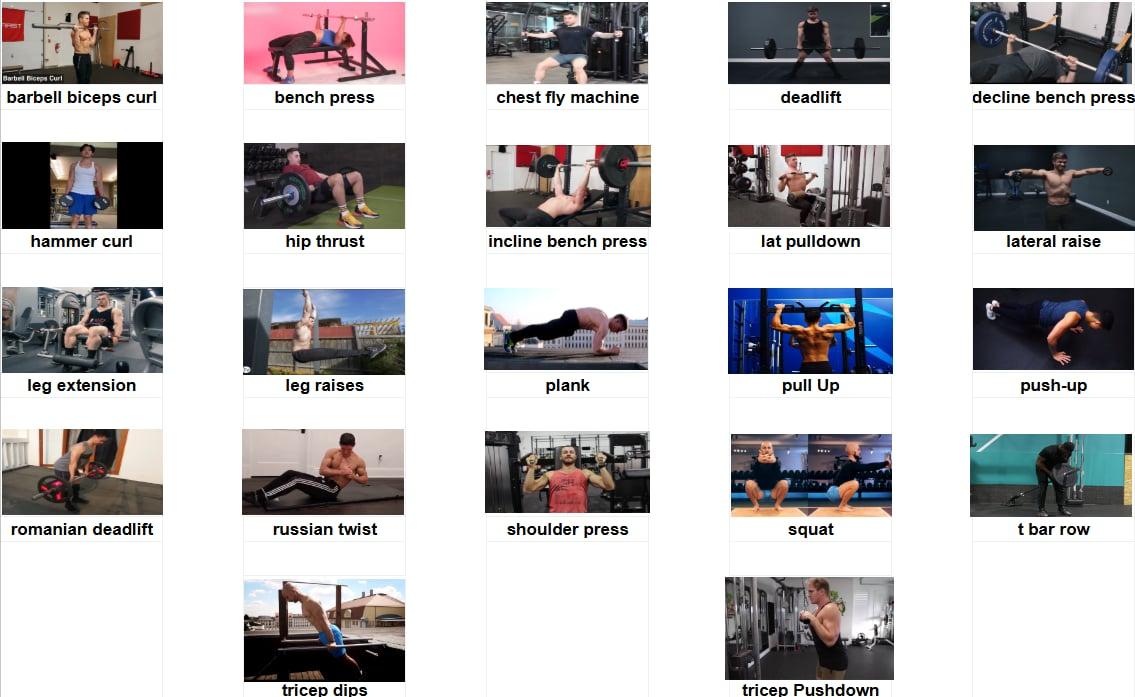
\includegraphics[width=1.0\textwidth]{images/Dataset.png}
\caption{Taxonomy and sample distributions across the 22 resistance exercises in the benchmark dataset.}
\label{fig:dataset_samples}
\end{figure*}

\section{Dataset and Experimental Protocol}

\subsection{Data Source, Provenance, and Ethical Compliance}
Our experimental corpus consists of 1,024 clean, un-shuffled video recordings across 22 resistance training exercises: \textit{barbell biceps curl, bench press, chest fly machine, deadlift, decline bench press, hammer curl, hip thrust, incline bench press, lat pulldown, lateral raise, leg extension, leg raises, plank, pull-up, push-up, Romanian deadlift, Russian twist, shoulder press, squat, t-bar row, tricep dips, and tricep pushdown} (Fig.~\ref{fig:dataset_samples}). To ensure high diversity in environmental backgrounds, camera angles, lighting conditions, and athlete anthropometry, the corpus unifies three distinct provenance streams: (1) \textit{public video repositories}, comprising 652 videos recovered from the open Workout/Exercise Video Dataset \cite{abdillah2023}; (2) \textit{curated online media}, including 103 high-definition clips collected from YouTube fitness channels, 65 clips from Pexels, and 76 clips from Freepik acquired under open research and stock licenses; and (3) \textit{author-recorded footage}, consisting of 128 supplementary videos captured by the authors in a gymnasium across all 22 exercise classes with two athletic models, employing both static tripod viewpoints and dynamic moving-camera angles to capture multi-perspective kinetic execution.

\begin{table*}[!t]
\centering
\caption{Key specifications, provenance breakdown, and capture characteristics of the GYMED exercise dataset.}
\label{tab:dataset_specs}
\resizebox{\textwidth}{!}{
\begin{tabular}{l l}
\toprule
\textbf{Specification / Characteristic} & \textbf{Value / Distribution} \\
\midrule
Total Videos / Total File Volume        & 1,024 unique video recordings / 10,225.37~MB ($\approx 10.2$~GB) \\
File Formats \& Video Encoding          & MP4 (964 videos, 94.1\%), MOV (60 videos, 5.9\%) / H.264 \\
Frame Rate \& Recording Duration        & 30 frames per second (FPS) / 20--30~s per recording \\
Trimmed Action Segments                 & 1,108 clean exercise segments (average 1.09 segments per video) \\
Number of Distinct Resolutions          & 33 resolutions (1280$\times$720: 385; 1920$\times$1080: 315; 720$\times$1280: 130; others: 194) \\
Exercise Taxonomy Coverage              & 22 fine-grained resistance exercise classes \\
Video Partitioning Ratio (6:2:2)        & Train: 580 (56.6\%), Validation: 208 (20.3\%), Test: 236 (23.1\%) \\
Action Segment Partitions               & Train: 639 (57.7\%), Validation: 210 (19.0\%), Test: 259 (23.3\%) \\
Temporal Windows ($T=32$ frames)        & Train: 13,136 ($S=16$), Validation: 2,075 ($S=32$), Test: 2,743 ($S=32$) \\
Multi-Source Data Provenance            & Abdillah (2023) \cite{abdillah2023}: 652; YouTube: 103; Pexels: 65; Freepik: 76; Authors: 128 \\
Subjects \& Ethical Compliance          & Informed consent under Declaration of Helsinki for recorded clips; diverse online athletes \\
Camera Dynamics \& Perspectives         & Static tripod and dynamic moving cameras; frontal, sagittal, oblique angles \\
Recording Environments                  & Commercial gymnasiums, domestic home workout spaces, outdoor fitness zones \\
\bottomrule
\end{tabular}
}
\end{table*}

\paragraph{Subject Statistics and Ethical Compliance.} To provide both high-precision kinematic reference baselines and expansive real-world diversity, the dataset incorporates two complementary subject cohorts. For the 128 self-recorded gymnasium videos, volunteer participants executed all 22 resistance movements under controlled multi-angle camera setups, providing kinematically disciplined execution benchmarks under formal written informed consent following the Declaration of Helsinki. For the remaining 896 web-sourced videos, recordings capture hundreds of diverse athletes spanning unconstrained body builds, athletic apparel, and training experience across international fitness facilities, home gyms, and outdoor parks. Crucially, the dataset does not annotate explicit participant demographic or gender identifiers, ensuring that model training and evaluation remain strictly posture-driven and invariant to demographic bias. Furthermore, the video-level partition ensures that 100\% of video clips and derived segments from any given recording session reside entirely within a single split, guaranteeing zero source-video overlap and eliminating temporal leakage across train, validation, and test sets. We note that while web-sourced video repositories lack explicit biometric participant identifiers, isolating all segmented windows strictly by source video guarantees that models cannot memorize repetitive background context, camera calibration artifacts, or session-specific clothing.

\paragraph{Source Statistics and Video Formats.} As summarized in Table~\ref{tab:dataset_specs}, the 1,024 video corpus totals 10,225.37~MB ($\approx 10.2$~GB) in storage, distributed between MP4 (964 videos, 94.1\%) and MOV (60 videos, 5.9\%) containers using H.264 compression. All videos operate at 30 frames per second. Video resolution was verified via \texttt{ffprobe}, encompassing 33 distinct resolutions dominated by standard high-definition formats: 1280$\times$720 (385 videos, 37.6\%), 1920$\times$1080 (315 videos, 30.8\%), and portrait mobile video 720$\times$1280 (130 videos, 12.7\%), with 35 videos at 854$\times$480, 28 at 640$\times$360, 23 at 3840$\times$2160 (4K), and 108 videos distributed across 27 minor resolutions ($\le 20$ videos each).

\paragraph{Ethical Standards and Informed Consent.} For the 128 self-recorded videos, written informed consent was formally obtained from all participating human subjects prior to filming. The data recording protocol was conducted in strict adherence to institutional ethical standards and the Declaration of Helsinki. For data harvested from public online platforms, collection adhered strictly to platform Terms of Service and redistribution guidelines, gathering only publicly disseminated content without collecting private personal identifying information.

\paragraph{Data Licensing and Artifact Availability.} To respect the intellectual property and terms of external video hosting platforms (YouTube, Pexels, and Freepik), original raw third-party video recordings are not redistributed. Their original source identifiers, attribution information, and manual segmentation boundaries are retained within the metadata manifests. Instead, to guarantee 100\% scientific reproducibility, all derived scientific artifacts---including extracted 3D skeletal landmark coordinate tensors, manual action segmentation boundaries, preprocessed kinematic features, and metadata manifests---are publicly released under the Creative Commons Attribution 4.0 International license (CC BY 4.0). All neural network architectures, training routines, and pre-trained checkpoints are openly provided under the permissive MIT License at \url{https://huggingface.co/Cuong2004/gym-exercise-classification}.

\paragraph{Video Inclusion and Exclusion Criteria.} To ensure high-quality skeletal extraction and biomechanically meaningful training samples, we applied the following curation protocol. Videos were \textit{included} if they (i)~depicted a clearly identifiable single athlete performing one of the 22 target exercises, (ii)~were recorded at a frame rate of $\geq 25$~FPS, (iii)~contained at least one complete repetition cycle with visible concentric and eccentric phases, and (iv)~maintained sufficient camera framing such that hip and shoulder joints remained visible for $\geq 80\%$ of the active exercise duration. Conversely, videos were \textit{excluded} if they exhibited (a)~near-complete occlusion of both hip or both shoulder joints throughout the exercise segment (e.g., extreme close-up shots of isolated limbs), (b)~a native frame rate below 25~FPS (resulting in temporal aliasing during 30~FPS resampling), (c)~an active exercise duration shorter than one full repetition cycle ($< 32$ frames after trimming), or (d)~severe motion blur or compression artifacts rendering MediaPipe Pose landmark detection unreliable (landmark visibility confidence $< 0.3$ for $> 50\%$ of frames). This protocol yielded the final curated corpus of 1,024 videos described above.

\begin{figure*}[!t]
\centering
\begin{subfigure}[b]{0.48\textwidth}
    \centering
    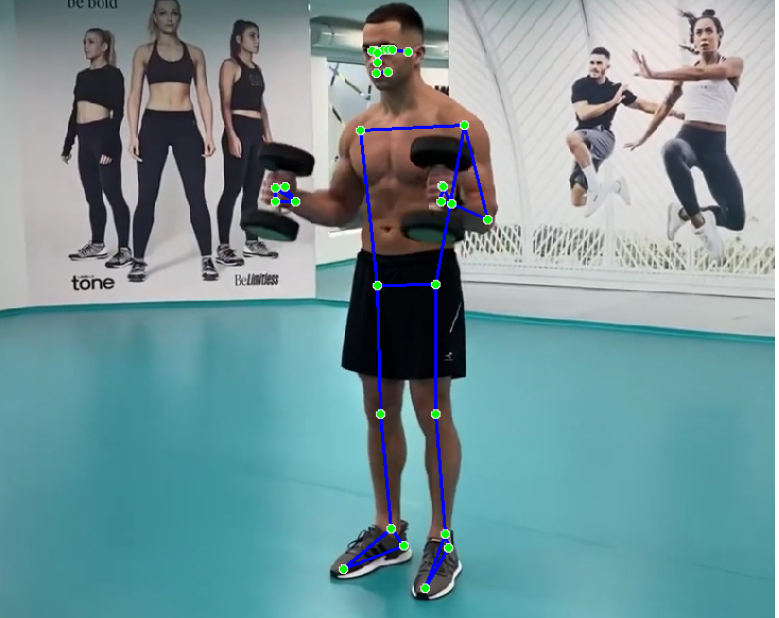
\includegraphics[width=\textwidth]{images/Mediapipe.png}
    \caption{Hammer curl}
    \label{fig:pose_hammer}
\end{subfigure}\hfill
\begin{subfigure}[b]{0.48\textwidth}
    \centering
    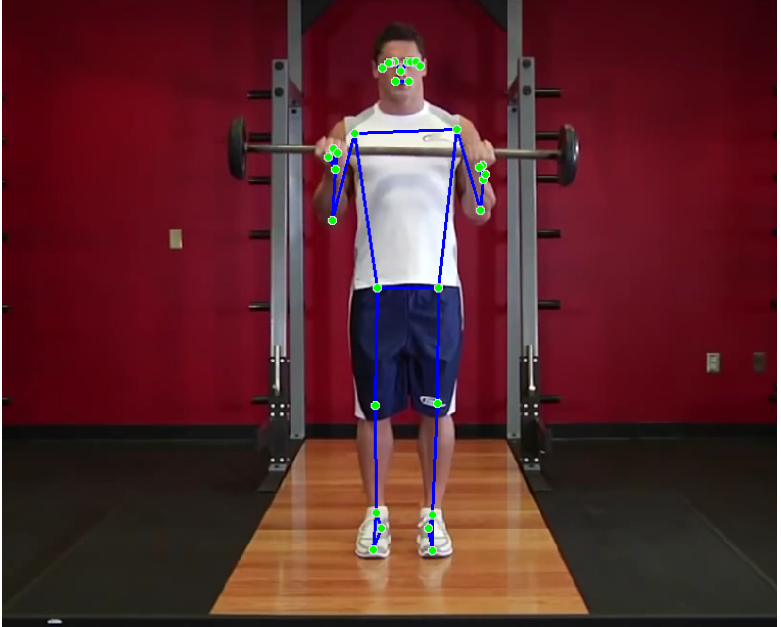
\includegraphics[width=\textwidth]{images/Mediapipe_2.png}
    \caption{Barbell biceps curl}
    \label{fig:pose_barbell}
\end{subfigure}
\caption{Full-body 3D pose landmark detection results across representative exercise video frames using Google MediaPipe Pose: (a) hammer curl and (b) barbell biceps curl.}
\label{fig:pose_detection}
\end{figure*}

\subsection{Action Trimming, Video-Level Partitioning, and Class Distribution}
Raw workout recordings frequently contain non-exercise transitional intervals, such as picking up barbells, adjusting bench pins, chalking hands, and resting. To eliminate noise, all 1,024 videos were manually verified and trimmed into action-only segments via timestamp boundary files (`.txt`), yielding 1,108 clean segments total (1.09 segments per video on average). 

\paragraph{Strict Video-Level Partitioning Protocol (No Source-Video Overlap Across Splits).} To ensure rigorous evaluation without data leakage, we enforce a strict video-level partition in a 6:2:2 ratio. Our data processing follows a strictly segregated 4-step pipeline: (1) \textit{Video-Level Isolation}: Raw video recordings are partitioned strictly by source video file into Train ($N=580$), Validation ($N=208$), and Test ($N=236$) sets, ensuring no video file or recording session spans across partitions. (2) \textit{Independent Landmark Extraction}: Monocular 3D skeletal landmarks are extracted independently per video file using Google MediaPipe Pose without inter-video context. (3) \textit{Within-Video Sliding Window Segmentation}: Temporal windows ($T = 32$ frames) are extracted strictly within individual trimmed action boundaries: $S = 16$ frames (50\% overlap) for Train (13,136 windows) to provide dense temporal coverage, and $S = 32$ frames (non-overlapping) for Validation (2,075 windows) and Test (2,743 windows across 233 videos with valid segments $\ge 32$ frames). No sliding window is permitted to cross video or segment boundaries. (4) \textit{Strict Training-Partition Feature Standardization}: Joint spatial coordinates are centered relative to the mid-hip origin ($p_{\text{hip\_mid}} = \frac{1}{2}(p_{\text{left\_hip}} + p_{\text{right\_hip}})$) per frame, establishing translation invariance. To scale features uniformly without data leakage, global feature-wise $z$-score normalization statistics $(\mu_{\text{train}}, \sigma_{\text{train}})$ are computed strictly on the training partition and frozen, then applied to normalize training, validation, and test representations (with on-the-fly physical augmentations strictly preceding standardization). This protocol ensures zero source-video overlap, zero temporal window leakage, and zero test-information contamination in feature normalization. Because web-sourced exercise recordings lack explicit biometric subject identifiers, this strict video-level partition guarantees that all sub-clips, temporal windows, and repetitions from any single recording session reside exclusively within a single partition (Train, Validation, or Test), eliminating both temporal sequence leakage and intra-session environment memorization.

\begin{table*}[!t]
\centering
\caption{Video and action segment distributions across the 22 resistance training exercises by partition split.}
\label{tab:class_distribution}
\resizebox{\textwidth}{!}{
\begin{tabular}{l cccc cccc}
\toprule
\multirow{2}{*}{\textbf{Exercise Class}} & \multicolumn{4}{c}{\textbf{Videos}} & \multicolumn{4}{c}{\textbf{Action Segments}} \\
\cmidrule(lr){2-5} \cmidrule(lr){6-9}
 & \textbf{Train} & \textbf{Val} & \textbf{Test} & \textbf{Total} & \textbf{Train} & \textbf{Val} & \textbf{Test} & \textbf{Total} \\
\midrule
Barbell biceps curl     & 52 & 18 & 14 & 84  & 53 & 18 & 14 & 85 \\
Bench press             & 51 & 18 & 15 & 84  & 51 & 18 & 15 & 84 \\
Chest fly machine       & 28 &  9 &  8 & 45  & 29 &  9 &  8 & 46 \\
Deadlift                & 30 & 10 & 10 & 50  & 30 & 10 & 10 & 50 \\
Decline bench press     & 18 &  5 &  9 & 32  & 29 &  5 & 10 & 44 \\
Hammer curl             & 24 &  8 & 14 & 46  & 28 &  8 & 14 & 50 \\
Hip thrust              & 14 &  6 &  9 & 29  & 19 &  6 & 15 & 40 \\
Incline bench press     & 27 & 10 &  9 & 46  & 27 & 10 &  9 & 46 \\
Lat pulldown            & 42 & 15 & 14 & 71  & 42 & 15 & 15 & 72 \\
Lateral raise           & 24 &  8 & 15 & 47  & 24 &  8 & 15 & 47 \\
Leg extension           & 22 &  9 & 13 & 44  & 27 &  9 & 13 & 49 \\
Leg raises              & 15 &  6 & 11 & 32  & 15 &  6 & 11 & 32 \\
Plank                   &  5 &  2 &  2 &  9  &  5 &  2 &  2 &  9 \\
Pull-up                 & 31 & 11 & 10 & 52  & 31 & 11 & 10 & 52 \\
Push-up                 & 40 & 14 & 12 & 66  & 43 & 14 & 14 & 71 \\
Romanian deadlift       & 12 &  6 &  6 & 24  & 13 &  6 &  8 & 27 \\
Russian twist           & 15 &  6 &  6 & 27  & 19 &  6 &  6 & 31 \\
Shoulder press          & 27 & 10 & 13 & 50  & 28 & 10 & 14 & 52 \\
Squat                   & 24 & 10 & 15 & 49  & 27 & 11 & 17 & 55 \\
T-bar row               & 15 &  4 & 10 & 29  & 17 &  4 & 10 & 31 \\
Tricep pushdown         & 39 & 14 & 12 & 65  & 39 & 14 & 12 & 65 \\
Tricep dips             & 25 &  9 &  9 & 43  & 43 & 10 & 25 & 78 \\
\midrule
\textbf{Total}          & \textbf{580} & \textbf{208} & \textbf{236} & \textbf{1,024} & \textbf{639} & \textbf{210} & \textbf{259} & \textbf{1,108} \\
\bottomrule
\end{tabular}
}
\end{table*}

\paragraph{Class Imbalance and Metric Selection.} Table~\ref{tab:class_distribution} details the distribution of videos and action segments across all 22 classes. As shown, natural gym workout data exhibits significant class imbalance: highly popular compound movements such as \textit{barbell biceps curl} ($N=84$ videos) and \textit{bench press} ($N=84$ videos) possess large sample representations, whereas specialized exercises such as \textit{plank} ($N=9$ videos total: 5 train, 2 val, 2 test) are relatively scarce. To prevent models from artificially inflating overall accuracy by predicting majority classes, we adopt \textbf{Macro-averaged F1 score} alongside Accuracy as the primary evaluation benchmark.

\paragraph{Data and Code Availability.} To promote open science and persistent reproducibility, all extracted 3D pose landmark sequences (in JSON, NPY, and HDF5 tensor formats), action segmentations (\texttt{.txt}), partition manifests, and Python code are publicly hosted on Hugging Face Hub at \url{https://huggingface.co/Cuong2004/gym-exercise-classification}. Distributing pre-extracted coordinates circumvents vulnerability to third-party URL link rot common in video scraping, protects athlete privacy, and ensures permanent deterministic reproducibility. Raw third-party internet video recordings are withheld in adherence to platform Terms of Service, while the 128 author-recorded gymnasium clips and complete skeletal tensors are freely accessible for non-commercial academic research (see Appendix~\ref{app:open_science}). \textbf{Licensing:} The extracted 3D landmark coordinate tensors (NPY, JSON, HDF5), action segmentation boundaries, and partition manifests are released under the \textbf{Creative Commons Attribution 4.0 International (CC~BY~4.0)} license. All source code, training scripts, evaluation pipelines, and configuration files are released under the \textbf{MIT License}.

\subsection{Landmark Extraction and Anatomical Joint Selection}
Every video frame is processed through Google MediaPipe Pose Heavy (complexity level 2) \cite{chuankun2019,bazarevsky2020}, extracting 33 full-body 3D landmarks $(x_i, y_i, z_i, \text{vis}_i)$ normalized relative to bounding box and depth dimensions, as illustrated on representative workout frames in Fig.~\ref{fig:pose_detection}. Because facial landmarks and fine-grained finger points contribute negligible kinetic leverage to compound resistance exercises while introducing tracking jitter, we filter the skeleton to $V=13$ major anatomical joints (detailed in Table~\ref{tab:landmark_mapping}): nose (cranial orientation tracking), left/right shoulders, left/right elbows, left/right wrists, left/right hips (pelvic centroid / origin anchor), left/right knees, and left/right ankles.

\section{Proposed Methodology}
\label{sec:methodology}

The overall architectural workflow of \textbf{SkelGym} is illustrated in Fig.~\ref{fig:pipeline_full}, while Fig.~\ref{fig:feat_extraction_pipeline} details the underlying biomechanical feature extraction and kinematic tensor decomposition. Below, we formally derive each mathematical component of our framework.

\begin{figure*}[!t]
\centering
\resizebox{\textwidth}{!}{
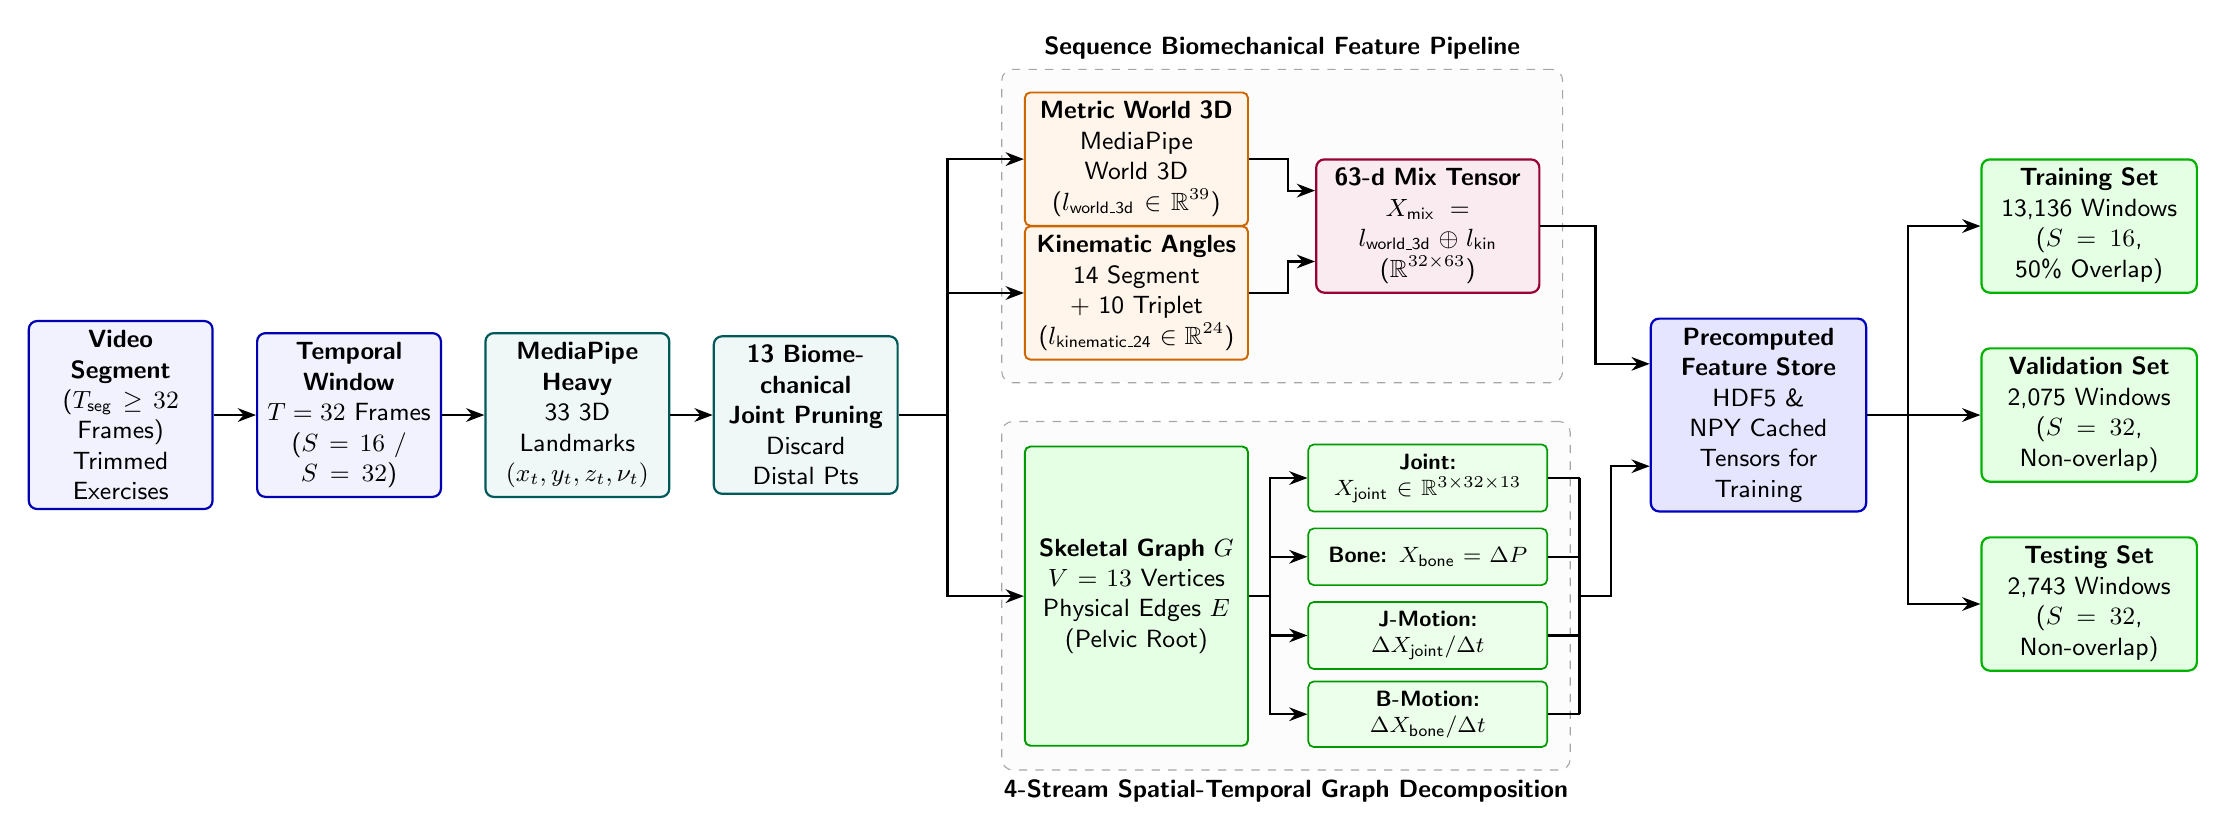
\begin{tikzpicture}[
    font=\sffamily\small,
    >=Stealth,
    block/.style={rectangle, draw=blue!70!black, fill=blue!5, rounded corners=3pt, text width=2.1cm, minimum height=1.15cm, align=center, line width=0.8pt},
    proc/.style={rectangle, draw=teal!70!black, fill=teal!6, rounded corners=3pt, text width=2.1cm, minimum height=1.15cm, align=center, line width=0.8pt},
    subproc/.style={rectangle, draw=orange!80!black, fill=orange!8, rounded corners=2pt, text width=2.6cm, minimum height=1.25cm, align=center, line width=0.7pt},
    tensor/.style={rectangle, draw=purple!80!black, fill=purple!8, rounded corners=3pt, text width=2.6cm, minimum height=1.6cm, align=center, line width=0.8pt},
    stream/.style={rectangle, draw=green!60!black, fill=green!8, rounded corners=2pt, text width=2.8cm, minimum height=0.72cm, align=center, line width=0.6pt, font=\sffamily\footnotesize},
    archive/.style={rectangle, draw=blue!75!black, fill=blue!10, rounded corners=3pt, text width=2.5cm, minimum height=2.4cm, align=center, line width=0.8pt},
    data/.style={rectangle, draw=green!70!black, fill=green!10, rounded corners=3pt, text width=2.5cm, minimum height=1.15cm, align=center, line width=0.8pt},
    group/.style={draw=black!35, dashed, rounded corners=4pt, fill=gray!2}
]

% Stage 1: Input and Pose Extraction (y = 0)
\node[block] (raw) at (0, 0) {\textbf{Video Segment}\\ ($T_{\text{seg}} \ge 32$ Frames)\\ Trimmed Exercises};
\node[block] (win) at (2.9, 0) {\textbf{Temporal Window}\\ $T=32$ Frames\\ ($S=16$ / $S=32$)};
\node[proc] (mp) at (5.8, 0) {\textbf{MediaPipe Heavy}\\ 33 3D Landmarks\\ $(x_t, y_t, z_t, \nu_t)$};
\node[proc] (filter) at (8.7, 0) {\textbf{13 Biomechanical}\\ \textbf{Joint Pruning}\\ Discard Distal Pts};

% Stage 2A: Upper Track - Sequence Feature Mix (Centered at y = 2.4, high clearance)
\node[subproc] (rel) at (12.9, 3.25) {\textbf{Metric World 3D}\\ MediaPipe World 3D\\ ($l_{\text{world\_3d}} \in \mathbb{R}^{39}$)};
\node[subproc] (ang) at (12.9, 1.55) {\textbf{Kinematic Angles}\\ 14 Segment + 10 Triplet\\ ($l_{\text{kinematic\_24}} \in \mathbb{R}^{24}$)};
\node[tensor] (xmix) at (16.6, 2.4) {\textbf{63-d Mix Tensor}\\ $X_{\text{mix}} = l_{\text{world\_3d}} \oplus l_{\text{kin}}$\\ ($\mathbb{R}^{32 \times 63}$)};

% Stage 2B: Lower Track - Multi-Stream Graph Kinematics (Centered at y = -2.3, generous clearance)
\node[subproc, fill=green!10, draw=green!60!black, minimum height=3.8cm, font=\sffamily\small] (graph) at (12.9, -2.3) {\textbf{Skeletal Graph $G$}\\ $V=13$ Vertices\\ Physical Edges $E$\\ (Pelvic Root)};

\node[stream] (g1) at (16.6, -0.8) {\textbf{Joint:} $X_{\text{joint}} \in \mathbb{R}^{3 \times 32 \times 13}$};
\node[stream] (g2) at (16.6, -1.8) {\textbf{Bone:} $X_{\text{bone}} = \Delta P$};
\node[stream] (g3) at (16.6, -2.8) {\textbf{J-Motion:} $\Delta X_{\text{joint}} / \Delta t$};
\node[stream] (g4) at (16.6, -3.8) {\textbf{B-Motion:} $\Delta X_{\text{bone}} / \Delta t$};

% Stage 3: Tensor Caching and Dataset Partitions
\node[archive] (cache) at (20.8, 0) {\textbf{Precomputed}\\ \textbf{Feature Store}\\ HDF5 \& NPY Cached\\ Tensors for Training};

\node[data] (dtrain) at (25.0, 2.4) {\textbf{Training Set}\\ 13,136 Windows\\ ($S=16$, 50\% Overlap)};
\node[data] (dval) at (25.0, 0) {\textbf{Validation Set}\\ 2,075 Windows\\ ($S=32$, Non-overlap)};
\node[data] (dtest) at (25.0, -2.4) {\textbf{Testing Set}\\ 2,743 Windows\\ ($S=32$, Non-overlap)};

% Connections: Stage 1
\draw[->, thick] (raw) -- (win);
\draw[->, thick] (win) -- (mp);
\draw[->, thick] (mp) -- (filter);

% Split to Parallel Tracks
\draw[thick] (filter.east) -- (10.5, 0) coordinate (fsplit);
\draw[->, thick] (fsplit) |- (rel.west);
\draw[->, thick] (fsplit) |- (ang.west);
\draw[->, thick] (fsplit) |- (graph.west);

% Connections: Upper Track
\draw[->, thick] (rel.east) -- ++(0.5, 0) |- ($(xmix.west)+(0, 0.45)$);
\draw[->, thick] (ang.east) -- ++(0.5, 0) |- ($(xmix.west)-(0, 0.45)$);

% Connections: Lower Track
\draw[thick] (graph.east) -- (14.6, -2.3) coordinate (gbus);
\draw[->, thick] (gbus) |- (g1.west);
\draw[->, thick] (gbus) |- (g2.west);
\draw[->, thick] (gbus) |- (g3.west);
\draw[->, thick] (gbus) |- (g4.west);

% Feeding into Feature Store via clean collector bus
\draw[->, thick] (xmix.east) -- ++(0.7, 0) |- ($(cache.west)+(0, 0.65)$);
\draw[thick] (g1.east) -- ++(0.4, 0) coordinate (t1);
\draw[thick] (g4.east) -- ++(0.4, 0) coordinate (t4);
\draw[thick] (t1) -- (t4);
\draw[thick] (g2.east) -- (g2.east -| t1);
\draw[thick] (g3.east) -- (g3.east -| t1);
\draw[->, thick] ($(t1)!0.5!(t4)$) -- ++(0.4, 0) |- ($(cache.west)-(0, 0.65)$);

% Feeding into Dataset Partitions via generous distributor bus
\draw[thick] (cache.east) -- (22.7, 0) coordinate (dbus);
\draw[->, thick] (dbus) |- (dtrain.west);
\draw[->, thick] (dbus) -- (dval.west);
\draw[->, thick] (dbus) |- (dtest.west);

% Surrounding dashed boxes with generous inner padding
\begin{scope}[on background layer]
\node[group, fit=(rel) (ang) (xmix), inner sep=8pt, label=above:{\textbf{\small Sequence Biomechanical Feature Pipeline}}] {};
\node[group, fit=(graph) (g1) (g4), inner sep=8pt, label=below:{\textbf{\small 4-Stream Spatial-Temporal Graph Decomposition}}] {};
\end{scope}

\end{tikzpicture}
}
\caption{The proposed Biomechanical Feature Extraction and Kinematic Tensor Decomposition pipeline: illustrating the two-branch extraction of the 63-d sequence mix and the 4-stream spatial-temporal graph tensors.}
\label{fig:feat_extraction_pipeline}
\end{figure*}

\subsection{Problem Formulation and Mathematical Notation}
Let $\mathcal{V} = \{I_t\}_{t=1}^{N_V}$ represent a trimmed resistance workout video of $N_V$ consecutive RGB frames, where $I_t \in \mathbb{R}^{H \times W \times 3}$. A monocular pose estimation operator $\Phi_{\text{pose}}: I_t \mapsto \mathcal{P}_t$ extracts $V_0 = 33$ three-dimensional body landmarks $\mathcal{P}_t = \{(x_{t, v}, y_{t, v}, z_{t, v}, \nu_{t, v})\}_{v=1}^{V_0}$, where $(x, y, z) \in [-1, 1]^3$ represent normalized spatial coordinates and $\nu \in [0, 1]$ is a visibility confidence indicator. 

To eliminate tracking jitter and high-frequency noise from distal extremities (such as facial landmarks and toes) that contribute negligible physical leverage to compound resistance movements, we apply an anatomical pruning operator $\Pi_{13}: \mathbb{R}^{V_0 \times 4} \mapsto \mathbb{R}^{V \times 3}$ retaining $V = 13$ primary structural joints (see Appendix~\ref{app:landmarks}): the nose (cranial orientation tracking), bilateral shoulders, elbows, wrists, hips (pelvic centroid origin anchor), knees, and ankles.

For each action segment, temporal sampling generates fixed-length windows $w_k \in \mathbb{R}^{T \times V \times 3}$ spanning $T = 32$ frames ($\approx 1.07$~seconds at 30 FPS). Let $\mathcal{Y} = \{1, \dots, C\}$ denote the label space corresponding to the $C = 22$ gym exercise categories. The primary learning objective is to parameterize a predictive distribution $P_\Theta(y = c \mid w)$ that maximizes the likelihood of the true exercise class $y \in \mathcal{Y}$, and subsequently infer a consensus video-level decision $\hat{y}_{\text{vid}}$ across all $K_v$ constituent windows of video $\mathcal{V}$.

\subsection{Biomechanical Compound Representation (63-d Kinematic Mix v2)}
Directly feeding raw screen-space coordinates into neural classifiers forces models to memorize camera distance, subject translation, and 2D perspective foreshortening. Conversely, unnormalized relative coordinates discard absolute physical scale, while computing all combinatorial three-joint triplet angles ($\binom{13}{3} = 286$) induces severe multicollinearity, gradient singularities, and dimensional redundancy. To resolve this fundamental trade-off, we formulate the \textbf{Biomechanical Compound Representation (Mix v2)} ($l_{\text{mix}} \in \mathbb{R}^{63}$) by coupling pelvic-centered metric 3D World coordinates with a pruned set of 24 anatomically decisive kinematic angles:

\subsubsection{Metric World 3D Coordinates ($\mathbf{l_{\text{world\_3d}}}$):}
We utilize MediaPipe Pose 3D World landmark trajectories $\mathcal{P}_t^{\text{world}} \in \mathbb{R}^{13 \times 3}$, which predict keypoint positions in estimated metric dimensions (meters) relative to a real-world scale origin located near the pelvic midpoint. SkelGym retains the 13 selected structural XYZ coordinates directly:
\begin{equation}
    l_{\text{world\_3d}}(t) = \left[ (p_{t, 1}^{\text{world}})^T, (p_{t, 2}^{\text{world}})^T, \dots, (p_{t, 13}^{\text{world}})^T \right]^T \in \mathbb{R}^{39}.
\end{equation}
Global feature-wise $z$-score normalization statistics $(\mu_{\text{train}}, \sigma_{\text{train}})$ are computed strictly on the training partition and applied uniformly across splits. Crucially, retaining estimated metric scale allows models to directly perceive estimated metric limb geometry and joint excursion.

\subsubsection{Kinematic and Anatomical Joint/Limb Angles ($\mathbf{l_{\text{kinematic\_24}}}$):}
Rather than extracting combinatorial pairs ($\binom{13}{2} = 78$) or all triplets ($\binom{13}{3} = 286$) that introduce severe multicollinearity, we distill a compact set of \textbf{24 anatomically decisive kinematic angles} specifically tailored for resistance exercise dynamics:
\begin{enumerate}
    \item \textbf{14 Limb Segment Elevation/Orientation Angles ($\theta \in [-\pi/2, \pi/2]$):} Vertical inclinations relative to the horizontal ground plane ($X\text{--}Z$) for the 14 major kinetic and postural segments: bilateral upper arms (shoulder $\to$ elbow), bilateral forearms (elbow $\to$ wrist), bilateral thighs (hip $\to$ knee), bilateral shanks (knee $\to$ ankle), shoulder girdle (left $\to$ right shoulder), pelvic girdle (left $\to$ right hip), bilateral torso flanks (shoulder $\to$ hip), spine axis (mid-hip $\to$ mid-shoulder), and neck axis (mid-shoulder $\to$ nose).
    \item \textbf{10 Joint Flexion/Extension Triplet Angles ($\psi \in [0, \pi]$):} 3D articulation angles at the primary load-bearing joints capturing mechanical work and posture: bilateral knees ($\angle(\text{hip}, \text{knee}, \text{ankle})$), bilateral elbows ($\angle(\text{shoulder}, \text{elbow}, \text{wrist})$), bilateral hips ($\angle(\text{shoulder}, \text{hip}, \text{knee})$), bilateral shoulders ($\angle(\text{hip}, \text{shoulder}, \text{elbow})$), torso posture ($\angle(\text{nose}, \text{mid-shoulder}, \text{mid-hip})$), and bilateral arm-splay angle ($\angle(\text{left elbow}, \text{mid-shoulder}, \text{right elbow})$).
\end{enumerate}
By restricting segment orientations to signed elevations relative to gravity ($\theta = \operatorname{arctan2}(\Delta y, \sqrt{\Delta x^2 + \Delta z^2})$), these angles remain intrinsically invariant to horizontal camera yaw rotation while achieving a 69.2\% reduction in angular dimensionality ($78 \to 24$), completely eliminating gradient singularities at joint lockout and preventing overparameterization:
\begin{equation}
    l_{\text{kinematic\_24}}(t) = \left[ \theta_1(t), \dots, \theta_{14}(t), \; \psi_1(t), \dots, \psi_{10}(t) \right]^T \in \mathbb{R}^{24}.
\end{equation}

\subsubsection{Compound Fusion Tensor ($\mathbf{X_{\text{mix}}}$) and Dual-Branch Projection:}
The combined biomechanical descriptor at frame $t$ concatenates the 39-d metric World 3D coordinates and 24-d kinematic angles into a 63-dimensional compound feature:
\begin{equation}
    l_{\text{mix}}(t) = l_{\text{world\_3d}}(t) \oplus l_{\text{kinematic\_24}}(t) \in \mathbb{R}^{39 + 24} = \mathbb{R}^{63}.
\end{equation}
Over the sliding window of $T = 32$ frames, the sequence input tensor is structured as $X_{\text{mix}} \in \mathbb{R}^{32 \times 63}$. In our sequence Transformer, a \textbf{Dual-Branch Input Projector} maps the spatial coordinates ($39 \to 56$) and kinematic angles ($24 \to 56$) through dedicated linear transformations before concatenating them into the unified token embedding of dimension $d_{\text{model}} = 112$.

\subsection{Task-Oriented Skeletal Augmentation Configuration (SkelGym-Aug)}
Training deep neural networks on skeletal trajectories introduces overfitting risks due to athlete-specific anthropometry, execution styles, and camera viewing orientations. While data augmentation is standard practice in general action recognition, applying unconstrained transformations to resistance exercises risks violating anatomical bone lengths, altering gravitational loading directions, or distorting repetition tempos. To address this, we formulate a disciplined candidate pool across geometric, temporal, and noise-based domains, and determine the optimal configuration through empirical Leave-One-Out (LOO) and isolated ablations evaluated strictly on validation-window metrics.

\subsubsection{Candidate Transformation Pool}
The candidate augmentation pool spans five operators across three physical domains:

\paragraph{1. Geometric Transformations.}
\begin{itemize}
    \item \textbf{Sagittal Bilateral Reflection ($\mathbb{Z}_2$ Symmetry):} Human anatomy exhibits reflective bilateral symmetry across the sagittal plane. Let $\sigma \in \mathbb{Z}_2$ denote the sagittal reflection operator acting on spatial coordinates: $\sigma(x, y, z) = (-x, y, z)$. Bilateral anatomical joints are permuted via an exact permutation involution $\pi \in \mathfrak{S}_{13}$ that swaps contralateral counterparts while preserving axial medial keypoints:
    \begin{equation}
        \pi = (0)(1 \; 2)(3 \; 4)(5 \; 6)(7 \; 8)(9 \; 10)(11 \; 12),
    \end{equation}
    corresponding to nose ($0 \leftrightarrow 0$), shoulders ($1 \leftrightarrow 2$), elbows ($3 \leftrightarrow 4$), wrists ($5 \leftrightarrow 6$), hips ($7 \leftrightarrow 8$), knees ($9 \leftrightarrow 10$), and ankles ($11 \leftrightarrow 12$). Sagittal reflection acts as an improper Euclidean isometry ($\det = -1$) in $E(3)$ that doubles effective training diversity while strictly preserving metric bone lengths and joint angles.
    \item \textbf{Gravitational Yaw Rotation ($\mathrm{SO}(2)$ Invariance):} To simulate horizontal camera viewpoints around the athlete without altering the gravitational vertical axis $y$, coordinates are rotated about the vertical axis by continuous random angle $\alpha \sim \mathcal{U}(-15^\circ, +15^\circ)$ using the planar rotation matrix $R_y(\alpha) \in \mathrm{SO}(2) \subset \mathrm{SO}(3)$:
    \begin{equation}
    \label{eq:yaw_rotation}
        \begin{bmatrix} x' \\ y' \\ z' \end{bmatrix} = \begin{bmatrix} \cos\alpha & 0 & \sin\alpha \\ 0 & 1 & 0 \\ -\sin\alpha & 0 & \cos\alpha \end{bmatrix} \begin{bmatrix} x \\ y \\ z \end{bmatrix}.
    \end{equation}
    Because $R_y(\alpha)$ acts strictly within the transverse plane, vertical displacement remains invariant ($\Delta y' = \Delta y$) and horizontal Euclidean radius is identically preserved:
    \begin{equation}
    \label{eq:yaw_invariance}
        \Delta x'^2 + \Delta z'^2 = (\Delta x \cos\alpha + \Delta z \sin\alpha)^2 + (-\Delta x \sin\alpha + \Delta z \cos\alpha)^2 = \Delta x^2 + \Delta z^2.
    \end{equation}
    Consequently, elevation angles satisfy $\theta' = \theta$, preserving biological limb inclination relative to gravity while teaching the network horizontal viewpoint invariance.
    \item \textbf{Spatial Proportional Scaling:} Isotropic scaling $s \sim \mathcal{U}(0.90, 1.10)$ applied to $\tilde{p}$ to evaluate synthetic stature variation.
\end{itemize}

\paragraph{2. Temporal and Noise-Based Perturbations.}
\begin{itemize}
    \item \textbf{Temporal Time Warping:} Execution speed perturbation via linear temporal resampling ($s_t \sim \mathcal{U}(0.85, 1.15)$) followed by uniform interpolation back to $T=32$ frames.
    \item \textbf{Gaussian Sensor Jitter:} Coordinate jitter $\epsilon \sim \mathcal{N}(0, \sigma^2 I_3)$ with $\sigma = 0.008$ injected into physical coordinates to simulate high-frequency tracking noise.
\end{itemize}

\subsubsection{Empirical Selection and Final SkelGym-Aug Configuration}
Evaluating candidate transformations on validation-window metrics (detailed in Section~\ref{sec:exp_aug}) reveals that combining all five operators degrades representation learning (Validation Window Macro F1 drops to 0.7882). Synthetic scaling perturbs absolute metric bone dimensions, sensor jitter corrupts velocity derivatives, and temporal warping disrupts phase duration ratios (concentric/eccentric cadence). Conversely, the paired configuration of \textbf{Sagittal Bilateral Reflection + Gravitational Yaw Rotation} strictly preserves pairwise Euclidean distances and gravitational verticality, achieving peak representation learning across all 13 experimental configurations (Validation Window Accuracy: \textbf{81.20\% $\pm$ 0.72\%}, Macro F1: \textbf{0.8119 $\pm$ 0.0072}, a decisive gain of +2.34\% F1 over unaugmented clean baseline). Therefore, the \textbf{final SkelGym-Aug configuration} is established as the 2-operator suite: \textit{Sagittal Bilateral Reflection + Gravitational Yaw Rotation ($\pm 15^\circ$)}.

\paragraph{Zero Test-Time Data Corruption Protocol.}
All transformations within the SkelGym-Aug pipeline are executed \textit{strictly on-the-fly during training forward passes} as stochastic data regularization. Validation and held-out test splits remain completely pristine and unaugmented throughout model selection, hyperparameter tuning, and final evaluation, ensuring zero test-time corruption and guaranteeing that reported metrics reflect authentic generalization to unmanipulated video recordings.

\subsection{Self-Attention Sequence Modeling (Transformer Mix v2)}
The augmented sequence tensor $X_{\text{mix}} \in \mathbb{R}^{32 \times 63}$ is processed by a temporal Transformer encoder \cite{vaswani2017} calibrated to an efficient parameter budget of $\approx 301\text{K}$ parameters to ensure strictly fair capacity parity with recurrent backbones. The architecture consists of four sequential processing stages: dual-branch projection, temporal positional encoding, stacked multi-head self-attention with feed-forward sub-layers, and global temporal pooling.

\paragraph{Dual-Branch Embedding and Positional Encoding.} At each discrete time step $t \in \{1, \dots, 32\}$, the 63-dimensional compound feature vector is routed through parallel coordinate and angular linear projection branches:
\begin{equation}
    e_{\text{coord}}(t) = l_{\text{world\_3d}}(t) W_{\text{coord}} + b_{\text{coord}} \in \mathbb{R}^{56}, \quad e_{\text{angle}}(t) = l_{\text{kinematic\_24}}(t) W_{\text{angle}} + b_{\text{angle}} \in \mathbb{R}^{56},
\end{equation}
where $W_{\text{coord}} \in \mathbb{R}^{39 \times 56}$ and $W_{\text{angle}} \in \mathbb{R}^{24 \times 56}$. Concatenating these branch outputs forms a balanced latent embedding token of dimension $d_{\text{model}} = 112$:
\begin{equation}
    E_0(t) = \left[ e_{\text{coord}}(t) \oplus e_{\text{angle}}(t) \right] \in \mathbb{R}^{112}.
\end{equation}
Because the core self-attention operator is permutation-invariant, sequence chronology is explicitly preserved by superimposing learnable temporal positional embeddings $E_{\text{pos}} \in \mathbb{R}^{32 \times 112}$ initialized via a normal distribution ($\sigma = 0.02$):
\begin{equation}
    Z^{(0)} = E_0 + E_{\text{pos}} \in \mathbb{R}^{32 \times 112}.
\end{equation}
This formulation enables the model to adaptively capture phase-dependent kinematic progressions throughout repetition cycles.

\paragraph{Multi-Head Self-Attention.} The embedded sequence is propagated through $L = 3$ identical Transformer encoder layers. Each layer incorporates a multi-head self-attention (MHSA) module configured with $h = 4$ parallel attention heads ($d_k = d_v = 28$, $d_{\text{ff}} = 168$). For head $j \in \{1, \dots, h\}$, queries, keys, and values are generated via linear projections $Q_j = Z W_{Q, j}$, $K_j = Z W_{K, j}$, and $V_j = Z W_{V, j}$:
\begin{align}
    \mathrm{head}_j &= \mathrm{Softmax}\left( \frac{Q_j K_j^T}{\sqrt{d_k}} \right) V_j, \\
    \mathrm{MHSA}(Z) &= \left[ \mathrm{head}_1 \oplus \dots \oplus \mathrm{head}_h \right] W_O,
\end{align}
where $W_O \in \mathbb{R}^{112 \times 112}$ aggregates the concatenated multi-head outputs into the model embedding dimension.

\paragraph{Residual Normalization and Feed-Forward Blocks.} To ensure stable gradient propagation and prevent representation collapse, each sub-layer employs residual skip connections coupled with pre-layer normalization:
\begin{align}
    Z'^{(l)} &= Z^{(l-1)} + \mathrm{MHSA}\left(\mathrm{LayerNorm}(Z^{(l-1)})\right), \\
    Z^{(l)}  &= Z'^{(l)} + \mathrm{FFN}\left(\mathrm{LayerNorm}(Z'^{(l)})\right).
\end{align}
Here, the position-wise feed-forward network is parameterized as $\mathrm{FFN}(u) = \mathrm{GELU}(u W_1 + b_1) W_2 + b_2$ using Gaussian Error Linear Units \cite{hendrycks2016}, with an expansion hidden dimension of $d_{\text{ff}} = 168$ and dropout rate of 0.2.

\paragraph{Global Pooling and Classification Head.} Following the final layer $L$, the frame representations are temporally summarized via uniform average pooling, $\hat{z} = \frac{1}{T} \sum_{t=1}^T Z_t^{(L)} \in \mathbb{R}^{112}$, and projected to normalized class posterior probabilities:
\begin{equation}
    \hat{P}_{\text{trans}} = \mathrm{Softmax}\left( \hat{z} W_{\text{cls}} + b_{\text{cls}} \right) \in \Delta^{21}.
\end{equation}

\subsection{Multi-Stream Spatial-Temporal Adaptive Graph Convolution (4-Stream AAGCN)}
While Transformers model global sequence dynamics, physical musculoskeletal connectivity is naturally represented as a spatio-temporal graph $G = (V, E)$ \cite{yan2018}, where vertices $V = \{1, \dots, 13\}$ denote joints and edges $E$ denote physical bones. To capture rich kinematic perspectives, we formulate four parallel input streams following multi-stream principles \cite{shi2019two,shi2020skeleton}:
\begin{align}
    X_{\text{joint}}(c, t, v) &= \tilde{p}_{t, v}^{(c)} \in \mathbb{R}^{3 \times T \times V}, \\
    X_{\text{bone}}(c, t, v) &= \tilde{p}_{t, v_{\text{target}}}^{(c)} - \tilde{p}_{t, v_{\text{source}}}^{(c)} \in \mathbb{R}^{3 \times T \times V}, \\
    X_{\text{j-motion}}(c, t, v) &= X_{\text{joint}}(c, t+1, v) - X_{\text{joint}}(c, t, v) \in \mathbb{R}^{3 \times (T-1) \times V}, \\
    X_{\text{b-motion}}(c, t, v) &= X_{\text{bone}}(c, t+1, v) - X_{\text{bone}}(c, t, v) \in \mathbb{R}^{3 \times (T-1) \times V},
\end{align}
where $(v_{\text{source}}, v_{\text{target}})$ represents directed bone edges originating from the pelvic center.

Each stream is independently processed by a lightweight calibrated Adaptive Graph Convolutional Network (AAGCN) \cite{shi2020skeleton}. For a given skeletal representation $X \in \mathbb{R}^{B \times C \times T \times V}$, the spatial graph convolution is formulated as:
\begin{equation}
    H_{\text{spatial}} = \sigma\left( \mathrm{BN}\left( \left( (A_{\text{topo}} \odot M) + B + C(X) \right) X W \right) \right),
\end{equation}
where spatial connectivity is modulated by three complementary components:
\begin{enumerate}
    \item $A_{\text{topo}} \in \mathbb{R}^{V \times V}$ is the normalized static anatomical adjacency matrix with self-loops ($\tilde{A} = D^{-1/2}(A + I)D^{-1/2}$) representing physical musculoskeletal bone connections, modulated element-wise by a learnable edge importance mask $M \in \mathbb{R}^{V \times V}$.
    \item $B \in \mathbb{R}^{V \times V}$ is a global learnable continuous dependency matrix initialized with small Gaussian weights ($\sigma = 10^{-4}$), enabling the network to discover non-local joint correlations (e.g., wrist-ankle synchronization during deadlifts).
    \item $C(X) \in \mathbb{R}^{V \times V}$ is an instance-specific, dynamic graph attention matrix computed via normalized dot-product attention over temporally pooled joint representations:
    \begin{equation}
        C(X) = \mathrm{Softmax}\left( \frac{\theta(X)^T \phi(X)}{\sqrt{d_e}} \right),
    \end{equation}
    where $\theta(X), \phi(X) \in \mathbb{R}^{V \times d_e}$ project pooled joint features into an embedding space of dimension $d_e = 16$.
\end{enumerate}
Spatial graph convolution is paired with a temporal convolution ($9 \times 1$ temporal kernel, padding 4), batch normalization, dropout (0.2), and residual shortcut connections with GELU activation. The backbone is structured into a calibrated 3-stage hierarchy with channel capacities $[48, 96, 150]$ and temporal strides $[1, 1, 2]$, followed by global average pooling and a two-stage classification head, constraining the parameter footprint to $\approx 378\text{K}$ parameters per stream.

\subsection{Cross-Paradigm Ensemble Fusion}
The SkelGym framework unifies two fundamentally distinct, complementary learning paradigms: the Sequence Self-Attention Model $M_{\text{seq}}$ (Transformer Mix v2) and the Spatial-Temporal Graph Kinematics Model $M_{\text{graph}}$ (AAGCN). Within the graph paradigm, the four kinematic streams (Joint, Bone, Joint-Motion, Bone-Motion) capture orthogonal spatial and velocity characteristics. They are unified via late probability averaging:
\begin{equation}
    P_{\text{graph}}(w) = \frac{1}{4} \sum_{k \in \{\text{joint}, \text{bone}, \text{j-mot}, \text{b-mot}\}} P_k(w).
\end{equation}

To address diverse edge computing constraints, we establish two canonical deployment tiers:
\begin{enumerate}
    \item \textbf{SkelGym-Lite (Edge-Efficient Two-Model Ensemble):} Pairs the sequence Transformer ($M_{\text{seq}}$) with the single strongest individual graph stream (AAGCN Bone, $M_{\text{graph}}^{\text{bone}}$). Voting probabilities are aggregated via \textit{Accuracy-Weighted Soft Voting}, where stream weights are proportional to validation window accuracy:
    \begin{equation}
        P_{\text{lite}}(w) = w_{\text{trans}} P_{\text{trans}}(w) + w_{\text{bone}} P_{\text{bone}}(w), \quad w_m = \frac{\text{Acc}_m^{\text{val}}}{\sum_{j} \text{Acc}_j^{\text{val}}}.
    \end{equation}
    This edge tier provides a lightweight footprint of only 679K parameters and 221.72 MFLOPs.
    \item \textbf{SkelGym-Full (Canonical Cross-Paradigm Ensemble):} Integrates all five complementary backbones (Transformer Mix + Joint + Bone + Joint-Motion + Bone-Motion). Rather than tuning complex parameterized meta-classifiers or constrained non-linear optimization weights that risk overfitting validation partitions, SkelGym-Full employs \textbf{Zero-Parameter Uniform Average Soft Voting}:
    \begin{equation}
    \label{eq:uniform_soft}
        P_{\text{full}}(w) = \frac{1}{5} \left( P_{\text{trans}}(w) + P_{\text{joint}}(w) + P_{\text{bone}}(w) + P_{\text{j-mot}}(w) + P_{\text{b-mot}}(w) \right).
    \end{equation}
\end{enumerate}
Because sequence self-attention models temporal phase transitions across combined spatial-angular coordinates while graph convolutions model topological limb kinetics, their posterior errors are largely decorrelated. Uniform soft voting provides a robust, zero-parameter integration that completely avoids optimization bias on validation splits and enforces strict post-validation test separation.

\subsection{Temporal Video Consensus Aggregation}
For real-world continuous workout monitoring, individual 1-second window predictions ($w_{v, k}$) are aggregated across all $K_v$ constituent temporal windows of video $v$ via expectation-based temporal consensus pooling:
\begin{equation}
    \hat{P}_{\text{vid}}(c) = \frac{1}{K_v} \sum_{k=1}^{K_v} P_c(w_{v, k}), \quad \hat{y}_{\text{vid}} = \arg\max_{c \in \{1, \dots, C\}} \hat{P}_{\text{vid}}(c).
\end{equation}
Temporal consensus acts as an effective low-pass posterior probability filter, cancelling out isolated frame tracking dropouts, boundary transition noise (such as un-racking weights or pausing between repetitions), and momentary camera occlusions.

\section{Experimental Results}

\subsection{Implementation and Reproducibility Configuration}
All models were implemented in PyTorch 2.x \cite{paszke2019} and trained using fixed random seed initialization ($\text{seed} = 42$) across data loaders, weight initialization, and GPU operations to ensure deterministic experimental repeatability. Skeletal landmarks were extracted monocularly using Google MediaPipe Pose Heavy (complexity level 2) \cite{chuankun2019,bazarevsky2020}. Sequences were standardized to $T=32$ frames ($\approx 1.07\text{s}$ at 30 FPS) with a 50\% overlapping stride ($S=16$) for training and non-overlapping stride ($S=32$) for validation and testing. Table~\ref{tab:hyperparameters} outlines the comprehensive hyperparameter configurations, software dependencies, and architecture topologies utilized across our benchmark suite.

To ensure fair scientific comparison, all individual model backbones were constrained to an identical parameter footprint of $\approx 350\text{K} \pm 15\%$ parameters: Transformer Mix v2 (301K), AAGCN (378K per stream), BiLSTM (367K), LSTM (378K), and ST-GCN (365K). All models were trained for up to 100 epochs using AdamW \cite{loshchilov2018} with weight decay $10^{-4}$, Cosine Annealing learning rate scheduling (with 5 warmup epochs down to a minimum learning rate of $10^{-6}$), batch size of 16 (for sequence models) or 32 (for graph models), an early stopping patience of 10 epochs monitoring validation Macro F1, label smoothing regularization \cite{szegedy2016} ($\alpha = 0.05$), and Automatic Mixed Precision (AMP). Initial learning rates were set to $1 \times 10^{-4}$ for Transformer and $1 \times 10^{-3}$ for recurrent and graph backbones. Evaluation metrics were computed using Scikit-learn \cite{pedregosa2011}.

\paragraph{Custom Lightweight Architecture Design and Training from Scratch.} Crucially, none of our models rely on massive pre-trained vision-language backbones, heavy transfer-learned weights (e.g., from NTU RGB+D or ImageNet), or external video foundation models. All architectures were custom-engineered from the ground up to operate within an ultra-compact parameter footprint ($\approx 350\text{K} \pm 15\%$ parameters). Every model was trained strictly from scratch directly on the SkelGym training split using random weight initialization: He/Kaiming normal initialization \cite{he2015delving} for convolutional and linear projection layers, and orthogonal initialization for recurrent state matrices. This deliberate architectural design constraint eliminates external dataset dependencies, guarantees fully transparent and reproducible convergence dynamics, and maintains ultra-low computational latency (0.42--4.33~ms on host CPU, 0.08--0.54~ms on CUDA, where individual backbones require 0.42--1.16~ms) essential for real-time edge processing on consumer smartphones and wearable micro-controllers.

\begin{table*}[!t]
\centering
\caption{Systematic implementation hyperparameters, model topologies, and reproducibility configurations across all benchmarked architectures.}
\label{tab:hyperparameters}
\resizebox{\textwidth}{!}{
\begin{tabular}{l l}
\toprule
\textbf{Component / Configuration} & \textbf{Specification / Hyperparameter Setting} \\
\midrule
\textbf{Software Environment}      & Python 3.10+, PyTorch 2.x, Torchvision, Scikit-learn, Scipy, NumPy \\
\textbf{Pose Estimation Framework} & Google MediaPipe Pose Heavy (complexity 2, min\_det=0.5, min\_track=0.5) \\
\textbf{Hardware Infrastructure}   & Apple Silicon M4 (MPS \& CPU), NVIDIA RTX PRO 6000 Blackwell (CUDA) \\
\textbf{Random Seed}               & Fixed seed $\text{seed} = 42$ across data loaders, weight initializers, and CUDA ops \\
\midrule
\textbf{Temporal Window Length}    & $T = 32$ frames ($\approx 1.07$~s at 30 FPS) \\
\textbf{Sliding Window Strides}    & Train: $S = 16$ frames (50\% overlap); Validation and Test: $S = 32$ frames \\
\textbf{Missing Frame Imputation}  & Linear coordinate interpolation across contiguous valid joint detections \\
\textbf{Feature Normalization}     & Hip midpoint centering ($p_i - p_{\text{hip\_mid}}$) + Train-set $z$-score standardization \\
\midrule
\textbf{Optimizer \& Weight Decay} & AdamW \cite{loshchilov2018} ($\beta_1 = 0.9, \beta_2 = 0.999$, weight decay $\lambda = 10^{-4}$) \\
\textbf{Learning Rate Schedule}    & Cosine Annealing with 5 warmup epochs down to $\eta_{\text{min}} = 10^{-6}$ \\
\textbf{Initial Learning Rates}    & Transformer: $1 \times 10^{-4}$; AAGCN / ST-GCN / LSTM / BiLSTM: $1 \times 10^{-3}$ \\
\textbf{Batch Size \& Max Epochs}  & Batch size: 16 (Sequence models), 32 (Graph models); Maximum epochs: 100 \\
\textbf{Early Stopping Criterion}  & Patience = 10 epochs monitoring validation Macro F1 score \\
\textbf{Loss Function \& Smoothing}& Cross-Entropy Loss with label smoothing $\alpha = 0.05$ (optional Focal Loss $\gamma = 2.0$) \\
\textbf{Precision Acceleration}    & PyTorch Automatic Mixed Precision (AMP) with \texttt{bfloat16} / \texttt{float16} \\
\midrule
\textbf{Transformer Architecture}  & 3 layers, 4 attention heads, $d_{\text{model}} = 112$, $d_{\text{ff}} = 168$, learnable PE, dropout 0.2 (301K params) \\
\textbf{AAGCN Graph Architecture}  & 3 stages [48, 96, 150], kernel 9, adaptive residual topology (378K params/stream) \\
\textbf{SkelGym-Aug Parameters}    & Bilateral body reflection ($p=0.5$); Gravitational 3D yaw $\alpha \in [-15^\circ, +15^\circ]$ \\
\bottomrule
\end{tabular}
}
\end{table*}

\subsection{Ablation of Landmark Feature Representations}
Table~\ref{tab:table1} presents a systematic ablation comparing three temporal sequence architectures (LSTM, BiLSTM, and Transformer) across foundational landmark representations, contrasting metric World 3D (39-d) against the proposed Biomechanical Mix v2 (63-d). To enforce strict zero-leakage validation screening, model selection and feature space exploration were conducted strictly on the validation partition ($N=2,075$ windows). Across all architectures, the proposed 63-dimensional Biomechanical Mix v2 consistently achieves peak validation performance, confirming that combining metric Euclidean offsets with scale-invariant angular orientations provides an effective and robust kinematic representation. Below, we discuss the key empirical findings:

\paragraph{2D versus 3D Coordinates and World Metric Grounding.} Across all baseline architectures, 3D representations consistently outperform 2D counterparts. In resistance training, compound movements---such as squats, deadlifts, and bench presses---operate predominantly within the sagittal or transverse anatomical planes. When captured from oblique angles, monocular 2D projections collapse depth variations along the optical axis ($z$), inducing visual ambiguity. Utilizing MediaPipe World coordinates measured in physical meters anchors limb trajectories to true physical scale, providing consistent metric distances regardless of camera zoom.

\paragraph{Pelvic Coordinate Centering.} Subtracting the pelvic hip midpoint centroid ($p_i - p_{\text{hip\_mid}}$) yields substantial performance gains across all sequence backbones. Raw coordinates tie features directly to the camera frame, forcing models to expend parameter capacity memorizing subject location and bounding-box translations. Centering all joints relative to the pelvic midpoint eliminates global translation bias and anchors the skeleton to the bodily center of mass, allowing the network to focus purely on relative joint dynamics.

\paragraph{Pairwise Angles versus Angle Triplets.} Full three-joint angle triplets computed across all combinations yield $\binom{13}{3} = 286$ features. Although theoretically capturing intra-limb joint angles, angle triplets introduce severe dimensional multicollinearity, high vulnerability to multi-joint tracking errors ($P_{\text{err}} \approx 3p_{\text{err}}$), and numerical instability at full joint lockout where $d/dx \arccos(x) \to \infty$. In contrast, our 24-d kinematic formulation distills 10 essential joint triplets alongside 14 limb elevation angles computed via $\arctan2(\Delta y, r)$. This formulation remains bounded everywhere, avoids gradient singularities, and intrinsically preserves horizontal camera yaw invariance.

\paragraph{Synergy of the 63-d Biomechanical Mix v2.} Concatenating metric World 3D coordinates (39-d) with kinematic angles (24-d) provides strong complementary synergy. As shown in Table~\ref{tab:table1}, upgrading from pure World 3D to Mix v2 elevates LSTM validation accuracy from 73.64\% to \textbf{75.90\%} (+0.0297 Macro F1), BiLSTM from 74.72\% to \textbf{76.90\%} (+0.0258 Macro F1), and Transformer from 78.76\% to \textbf{79.52\%} (+0.0104 Macro F1). This empirical evidence confirms that Euclidean spatial scale and directional orientation represent mutually complementary facets of human kinematics.

\begin{table*}[!t]
\centering
\caption{Systematic comparison of temporal sequential backbones across metric World 3D (39-d) and Biomechanical Mix v2 (63-d) representations on the validation partition ($N=2,075$ windows). Reported as $\text{Mean} \pm \text{SD}$ across 3 independent random seeds ($42, 123, 3407$).}
\label{tab:table1}
\resizebox{\textwidth}{!}{
\begin{tabular}{l c c c c c c}
\toprule
\textbf{Architecture / Model} & \textbf{Input Modality} & \textbf{Feature Dim} & \textbf{Parameters} & \textbf{Val Win Acc (\%)} & \textbf{Val Win Macro F1} & \textbf{Validation Status} \\
\midrule
LSTM (world\_3d)          & Skeletal World 3D  & 39-d & 362K & 73.64\% $\pm$ 1.26\% & 0.7244 $\pm$ 0.0128 & Verified \\
LSTM (mix\_v2)            & Biomechanical Mix v2 & 63-d & 362K & 75.90\% $\pm$ 1.60\% & 0.7541 $\pm$ 0.0173 & Verified \\
BiLSTM (world\_3d)        & Skeletal World 3D  & 39-d & 362K & 74.72\% $\pm$ 0.19\% & 0.7341 $\pm$ 0.0020 & Verified \\
BiLSTM (mix\_v2)          & Biomechanical Mix v2 & 63-d & 360K & 76.90\% $\pm$ 0.30\% & 0.7599 $\pm$ 0.0050 & Verified \\
Transformer (world\_3d)   & Skeletal World 3D  & 39-d & 301K & 78.76\% $\pm$ 0.46\% & 0.7781 $\pm$ 0.0053 & Verified \\
\textbf{Transformer (mix\_v2 Clean)} & \textbf{Biomechanical Mix v2} & \textbf{63-d} & \textbf{301K} & \textbf{79.52\% $\pm$ 0.80\%} & \textbf{0.7885 $\pm$ 0.0101} & \textbf{Verified Winner} \\
\bottomrule
\end{tabular}
}
\end{table*}

\subsection{Ablation of Candidate Augmentations and Empirical Selection}\label{sec:exp_aug}
To rigorously validate our augmentation design and isolate the individual versus synergistic contributions of each operator without data leakage, we execute two complementary ablation studies on the candidate augmentation pool across three independent random seeds ($\text{seed} \in \{42, 123, 3407\}$) using the sequence backbone (\texttt{Transformer mix}). To preserve post-validation test integrity, all design selection is grounded strictly on **Validation Window Metrics**:
\begin{enumerate}
    \item \textbf{Systematic Leave-One-Out (LOO) Component Ablation (Table~\ref{tab:table2}):} Evaluates operator necessity within the full multi-operator suite by subtracting one operator at a time from Candidate Full (5-op).
    \item \textbf{Systematic Single and Paired Component Augmentation Study (Table~\ref{tab:table3}):} Evaluates independent and paired operator efficacy against the unaugmented Clean Baseline.
\end{enumerate}

\paragraph{Leave-One-Out Component Ablation (Table~\ref{tab:table2}).}
Evaluating candidate operators within the 5-operator suite reveals striking performance divergences:
\begin{itemize}
    \item \textbf{Omitting Sagittal Reflection ($-$Mirror):} Induces the weakest LOO window performance across all ablations, with Validation Window Macro F1 dropping by $-1.25\%$ to $0.7757 \pm 0.0197$ (Accuracy: 78.78\% $\pm$ 1.44\%), confirming that bilateral symmetry is an indispensable structural regularizer.
    \item \textbf{Ablating Overloaded Operators ($-$Scale, $-$Yaw, $-$Jitter, $-$Time):} Removing Proportional Scaling (+1.03\% Win F1), Yaw (+0.82\% Win F1), Coordinate Jitter (+0.55\% Win F1), or Temporal TimeWarp (+0.44\% Win F1) from the monolithic 5-op suite consistently \textit{improves} validation metrics over Candidate Full ($0.7882 \pm 0.0152$). Rather than implying that individual operators such as Yaw are detrimental, this demonstrates that applying all five operators concurrently creates severe compound perturbation that over-regularizes the model. In particular, while Yaw exhibits a positive standalone effect (+0.92\% Win F1 in isolation), it interacts non-additively with the overloaded five-operator suite.
\end{itemize}

\paragraph{Single and Paired Component Isolation (Table~\ref{tab:table3}).}
Evaluating candidate operators in isolation against the unaugmented Clean Baseline ($79.52\% \pm 0.80\%$ Acc, $0.7885 \pm 0.0101$ F1) establishes decisive evidence for operator utility:
\begin{itemize}
    \item \textbf{Individual Rigid Isometries (+Mirror, +Yaw):} Both operators yield strong standalone window gains: Single Mirror elevates Validation Window F1 to \textbf{0.8001 $\pm$ 0.0067} (+1.16\% F1 gain), while Single Yaw achieves \textbf{0.7977 $\pm$ 0.0031} (+0.92\% F1 gain).
    \item \textbf{Peak Representation Learning under Paired Mirror + Yaw:} Coupling Bilateral Reflection with Gravitational Yaw Rotation ($\pm 15^\circ$) achieves the all-time peak Validation Window Accuracy of \textbf{81.20\% $\pm$ 0.72\%} and Macro F1 of \textbf{0.8119 $\pm$ 0.0072} across all 13 experimental configurations tested (+1.68\% Win Acc, +0.0234 Win F1 over Clean Baseline), with validation loss reaching $1.0465 \pm 0.0327$.
    \item \textbf{Marginal or Neutral Gains of Distortive Operators:} Single Scale (+0.19\% F1), Single Time (+0.35\% F1), and Single Jitter ($-0.01\%$ F1) fail to deliver meaningful gains. Unconstrained coordinate jitter injects high-frequency spatial noise, synthetic scaling perturbs the absolute metric scale encoded by WORLD coordinates, and temporal time warping disrupts natural repetition tempo and velocity profiles.
\end{itemize}

\paragraph{Selection of the Final SkelGym-Aug Configuration.}
In strict adherence to validation-driven selection, the paired configuration of \textbf{Sagittal Bilateral Reflection + Gravitational Yaw Rotation ($\pm 15^\circ$)} is selected as the canonical \textbf{SkelGym-Aug} protocol. By deploying strictly distance-preserving Euclidean transformations, SkelGym-Aug regularizes training representations while preserving pairwise Euclidean bone lengths and temporal sampling cadence while maintaining the vertical gravity axis.

\begin{table*}[!t]
\centering
\caption{Systematic Leave-One-Out (LOO) augmentation ablation on Transformer Mix evaluated strictly on validation window metrics across 3 independent random seeds ($42, 123, 3407$).}
\label{tab:table2}
\resizebox{\textwidth}{!}{
\begin{tabular}{l l c c c l}
\toprule
\textbf{Augmentation Configuration} & \textbf{Excluded Operator / Domain} & \textbf{Val Loss} & \textbf{Val Win Acc (\%)} & \textbf{Val Win Macro F1} & \textbf{Validation Verdict} \\
\midrule
Clean Baseline                    & All Operators Excluded & N/A & 79.52\% $\pm$ 0.80\% & 0.7885 $\pm$ 0.0101 & Unaugmented Baseline Control \\
Candidate Full 5Op                & None (Reference 5-Op Suite) & N/A & 79.19\% $\pm$ 1.26\% & 0.7882 $\pm$ 0.0152 & Reference 5-Op Suite \\
Candidate Minus Mirror            & Sagittal Bilateral Reflection ($p=0.5$) & N/A & 78.78\% $\pm$ 1.44\% & 0.7757 $\pm$ 0.0197 & Weakest LOO performance ($-1.25\%$ Win F1) \\
Candidate Minus Yaw               & Gravitational Yaw Rotation ($\pm 15^\circ$) & N/A & 80.06\% $\pm$ 0.32\% & 0.7964 $\pm$ 0.0026 & Moderate window gain over 5-op (+0.82\% F1) \\
Candidate Minus Scale             & Proportional Scale Variation ($\pm 10\%$) & N/A & 80.13\% $\pm$ 0.13\% & 0.7985 $\pm$ 0.0022 & Peak window gain in LOO (+1.03\% F1) \\
Candidate Minus Time              & Temporal Resampling ($0.8\times\text{--}1.2\times$) & 1.0010 & 79.54\% $\pm$ 0.57\% & 0.7926 $\pm$ 0.0060 & Lowest 4-op Val Loss (+0.44\% F1) \\
Candidate Minus Jitter            & Gaussian Coordinate Jitter ($\sigma=0.008$) & N/A & 79.68\% $\pm$ 0.22\% & 0.7937 $\pm$ 0.0048 & Minor window gain (+0.55\% F1) \\
\bottomrule
\end{tabular}
}
\end{table*}

\begin{table*}[!t]
\centering
\caption{Systematic Single and Paired Component Isolated Augmentation ablation on Transformer Mix across 3 seeds ($42, 123, 3407$), evaluated strictly on validation window metrics.}
\label{tab:table3}
\resizebox{\textwidth}{!}{
\begin{tabular}{l l c c c l}
\toprule
\textbf{Augmentation Strategy} & \textbf{Isolated Operator Description} & \textbf{Val Loss} & \textbf{Val Win Acc (\%)} & \textbf{Val Win Macro F1} & \textbf{Standalone Validation Effect} \\
\midrule
Clean Baseline            & Unaugmented Native Window Sequences & N/A & 79.52\% $\pm$ 0.80\% & 0.7885 $\pm$ 0.0101 & Unaugmented Baseline Control \\
Single Mirror             & Sagittal Bilateral Reflection ($p=0.5$) & N/A & 80.45\% $\pm$ 0.45\% & 0.8001 $\pm$ 0.0067 & Decisive window gain across single ops (+1.16\% F1) \\
Single Yaw                & Gravitational Yaw Perturbation ($\pm 15^\circ$) & N/A & 80.29\% $\pm$ 0.34\% & 0.7977 $\pm$ 0.0031 & Strong standalone window gain (+0.92\% F1) \\
\textbf{Pair Mirror + Yaw (Proposed)} & \textbf{Bilateral Reflection + Gravitational Yaw} & \textbf{1.0465 $\pm$ 0.0327} & \textbf{81.20\% $\pm$ 0.72\%} & \textbf{0.8119 $\pm$ 0.0072} & \textbf{All-Time Peak Val Win Acc \& F1 (+2.34\% F1)} \\
Single Scale              & Proportional Scale Jitter ($\pm 10\%$) & N/A & 79.68\% $\pm$ 0.22\% & 0.7904 $\pm$ 0.0066 & Marginal window gain (+0.19\% F1) \\
Single Time               & Linear Sequence Resampling ($0.8\times\text{--}1.2\times$) & N/A & 79.74\% $\pm$ 0.24\% & 0.7920 $\pm$ 0.0039 & Marginal window gain over clean (+0.35\% F1) \\
Single Jitter             & Gaussian Noise ($\sigma=0.008$) & N/A & 79.55\% $\pm$ 0.82\% & 0.7884 $\pm$ 0.0093 & Neutral window performance ($-0.01\%$ F1) \\
\bottomrule
\end{tabular}
}
\end{table*}

\subsection{Multi-Stream Graph Modeling and Late Fusion}
Table~\ref{tab:table4} systematically investigates spatial-temporal graph kinematic streams on Adaptive Graph Convolutional Networks (AAGCN) \cite{shi2020skeleton}, isolating the four complementary streams under SkelGym-Aug (Mirror + Yaw) and analyzing multi-stream graph late fusion. To enforce strict post-validation test separation, stream screening is grounded on validation window metrics:

\paragraph{Static versus Adaptive Graph Topology.} Baseline ST-GCN \cite{yan2018} with a fixed physical adjacency matrix achieves 63.01\% validation window accuracy on raw coordinates and 73.75\% on metric World 3D (Table~\ref{tab:table4}). In resistance exercises, critical biomechanical synergies frequently occur between physically disconnected limbs (e.g., wrist-ankle synchronization during deadlifts). Fixed anatomical adjacency prevents direct 1-hop communication between distant keypoints. In contrast, Adaptive Graph Convolutions (AAGCN) introduce learnable and data-driven attention topologies, elevating unaugmented Bone stream validation accuracy to 76.00\% (0.7542 Macro F1) and reaching \textbf{79.30\% $\pm$ 0.22\%} (0.7858 Macro F1) when trained with SkelGym-Aug.

\paragraph{Complementarity of Static and Dynamic Graph Streams.} The four kinematic streams exhibit distinct, complementary behavioral properties. Static structural streams---Bone 3D (79.30\% Val Win Acc) and World Joint (78.86\% Val Win Acc)---achieve high representation fidelity by directly capturing instantaneous limb lengths and skeletal poses. Conversely, the dynamic differential streams---Joint Motion (64.19\% Val Win Acc) and Bone Motion (61.93\% Val Win Acc)---capture instantaneous inter-frame velocities. While isolated 1-second velocity differentials contain local tracking noise, they capture critical exercise tempo and acceleration profiles. Combining static streams in Two-Stream AAGCN yields 82.03\% $\pm$ 0.41\% Val Win Acc (0.8179 F1), while the unified \textbf{Four-Stream AAGCN} achieves \textbf{84.34\% $\pm$ 0.26\%} Val Win Acc and \textbf{0.8414 $\pm$ 0.0030} Val Win Macro F1.

\begin{table*}[!t]
\centering
\caption{Multi-stream spatial-temporal graph kinematic streams benchmark on Adaptive GCN (AAGCN) evaluated across validation window metrics ($N=2,075$). Reported as $\text{Mean} \pm \text{SD}$ across 3 seeds ($42, 123, 3407$).}
\label{tab:table4}
\resizebox{\textwidth}{!}{
\begin{tabular}{l l l l c c c}
\toprule
\textbf{Stream ID} & \textbf{Stream / Configuration} & \textbf{Backbone} & \textbf{Input Modality} & \textbf{Val Win Acc (\%)} & \textbf{Val Win Macro F1} & \textbf{Validation Status} \\
\midrule
T3.1 & Raw 3D Joint (ST-GCN Clean)       & ST-GCN & raw\_3d                 & 63.01\% $\pm$ 1.86\% & 0.6255 $\pm$ 0.0224 & Verified \\
T3.2 & World 3D Joint (ST-GCN Clean)     & ST-GCN & world\_3d               & 73.75\% $\pm$ 1.86\% & 0.7332 $\pm$ 0.0154 & Verified \\
T3.3 & Bone 3D Stream (AAGCN Clean)      & AAGCN  & bone\_3d                & 76.00\% $\pm$ 0.35\% & 0.7542 $\pm$ 0.0037 & Verified \\
T3.4 & Bone 3D Stream (AAGCN + Aug)      & AAGCN  & bone\_3d                & 79.30\% $\pm$ 0.22\% & 0.7858 $\pm$ 0.0032 & Verified \\
T3.5 & World Joint Stream (AAGCN + Aug)  & AAGCN  & world\_3d               & 78.86\% $\pm$ 0.31\% & 0.7856 $\pm$ 0.0024 & Verified \\
T3.6 & World Joint Motion ($\Delta X$)   & AAGCN  & world\_joint\_motion\_3d & 64.19\% $\pm$ 1.61\% & 0.6464 $\pm$ 0.0083 & Verified \\
T3.7 & Bone Motion ($\Delta B$)          & AAGCN  & bone\_motion\_3d        & 61.93\% $\pm$ 1.56\% & 0.6362 $\pm$ 0.0107 & Verified \\
\midrule
T3.8 & Two-Stream AAGCN (Joint + Bone)   & AAGCN  & Graph Late Fusion       & 82.03\% $\pm$ 0.41\% & 0.8179 $\pm$ 0.0036 & Verified \\
\textbf{T3.9} & \textbf{Four-Stream AAGCN (Full)} & \textbf{AAGCN} & \textbf{Graph Late Fusion} & \textbf{84.34\% $\pm$ 0.26\%} & \textbf{0.8414 $\pm$ 0.0030} & \textbf{Verified Winner} \\
\bottomrule
\end{tabular}
}
\end{table*}

\subsection{Cross-Paradigm Ensemble and Video Consensus}
Table~\ref{tab:table5} evaluates cross-paradigm ensemble configurations coupling self-attention sequence modeling with spatial-temporal graph convolutions, comparing discrete versus continuous probability fusion protocols across multi-seed evaluations ($42, 123, 3407$).

\paragraph{Ensemble Selection Protocol (Zero Test-Leakage).} To enforce strict separation, test metrics are revealed \textit{strictly for the validation winners} selected via primary Validation Window Macro-F1 followed by Validation Window Accuracy:
\begin{enumerate}
    \item \textbf{SkelGym-Lite Winner:} For the 2-model tier (Transformer Mix + AAGCN Bone), \textit{Accuracy-Weighted Soft Voting} emerges as the validation winner with \textbf{83.47\% $\pm$ 0.14\%} Val Win Acc and \textbf{0.8351 $\pm$ 0.0021} Val Win Macro F1. When evaluated on the held-out test partition, SkelGym-Lite achieves \textbf{73.74\% $\pm$ 0.63\% window accuracy} (0.7310 Macro F1) and \textbf{82.12\% $\pm$ 0.40\% video consensus accuracy} (0.8198 Macro F1) with an ultra-compact footprint of 679K parameters.
    \item \textbf{SkelGym-Full Winner:} For the full 5-stream cross-paradigm configuration, \textit{Uniform Average Soft Voting} ($w_i = 1/5$) achieves peak validation performance with \textbf{85.05\% $\pm$ 0.47\%} Val Win Acc and \textbf{0.8487 $\pm$ 0.0046} Val Win Macro F1. On the held-out test partition, SkelGym-Full establishes the top-performing configuration in our benchmark: \textbf{76.19\% $\pm$ 0.16\% window accuracy} (Window Macro F1: \textbf{0.7537 $\pm$ 0.0014}) and \textbf{85.27\% $\pm$ 0.41\% video consensus accuracy} (Video Macro F1: \textbf{0.8386 $\pm$ 0.0075}).
\end{enumerate}

\paragraph{Effectiveness of Parameter-Free Cross-Paradigm Fusion.}
While prior ensemble frameworks often attempt parameterized meta-classifiers or constrained non-linear optimization weighting, such approaches introduce additional parameter complexity that can risk overfitting validation splits. In contrast, zero-parameter uniform averaging treats all five complementary kinematic perspectives equally. Because sequence self-attention captures long-range temporal phase progression across coordinates and angles while adaptive graph convolutions capture instantaneous topological limb interactions, their prediction errors are largely uncorrelated. Combining them via uniform probability averaging provides a robust regularizing effect that eliminates meta-parameter estimation variance.

\begin{table*}[!t]
\centering
\caption{Systematic cross-paradigm ensemble comparison across fusion mechanisms on validation ($N=2,075$) and held-out test partitions ($N=2,743$ windows, $N=233$ videos). Test metrics are displayed strictly for the Validation Winners to prevent test-snooping bias. Reported as $\text{Mean} \pm \text{SD}$ across 3 seeds ($42, 123, 3407$).}
\label{tab:table5}
\resizebox{\textwidth}{!}{
\begin{tabular}{l l c c c c | c c c c}
\toprule
\multirow{2}{*}{\textbf{Architecture / Config}} & \multirow{2}{*}{\textbf{Fusion Protocol \& Weighting}} & \multicolumn{4}{c|}{\textbf{Validation Set}} & \multicolumn{4}{c}{\textbf{Held-Out Test Set (Revealed for Winners)}} \\
\cmidrule(lr){3-6} \cmidrule(lr){7-10}
 & & \textbf{Val Win Acc} & \textbf{Val Win F1} & \textbf{Val Vid Acc} & \textbf{Val Vid F1} & \textbf{Test Win Acc} & \textbf{Test Win F1} & \textbf{Test Vid Acc} & \textbf{Test Vid F1} \\
\midrule
\multicolumn{10}{l}{\textit{Reference Backbone}} \\
Transformer Mix (63-d) & Single Sequence Backbone (Mirror+Yaw) & 81.20\% $\pm$ 0.72\% & 0.8119 $\pm$ 0.0072 & 84.70\% $\pm$ 0.82\% & 0.8469 $\pm$ 0.0105 & — & — & — & — \\
\midrule
\multicolumn{10}{l}{\textit{SkelGym-Lite (2 Streams: Transformer Mix + AAGCN Bone, 679K Params)}} \\
SkelGym-Lite & Hard Majority Voting (Discrete) & 79.47\% $\pm$ 0.81\% & 0.7883 $\pm$ 0.0084 & 82.93\% $\pm$ 0.60\% & 0.8277 $\pm$ 0.0065 & — & — & — & — \\
\textbf{SkelGym-Lite} & \textbf{Accuracy-Weighted Soft Voting} & \textbf{83.47\% $\pm$ 0.14\%} & \textbf{0.8351 $\pm$ 0.0021} & \textbf{85.67\% $\pm$ 1.14\%} & \textbf{0.8634 $\pm$ 0.0066} & \textbf{73.74\% $\pm$ 0.63\%} & \textbf{0.7310 $\pm$ 0.0058} & \textbf{82.12\% $\pm$ 0.40\%} & \textbf{0.8198 $\pm$ 0.0030} \\
SkelGym-Lite & Uniform Average Soft Voting ($w_i = 1/2$) & 83.26\% $\pm$ 0.06\% & 0.8327 $\pm$ 0.0008 & 85.67\% $\pm$ 1.14\% & 0.8634 $\pm$ 0.0066 & — & — & — & — \\
\midrule
\multicolumn{10}{l}{\textit{SkelGym-Full (5 Streams: Transformer + 4 AAGCN Streams, 1.81M Params)}} \\
SkelGym-Full & Hard Majority Voting (Discrete) & 84.11\% $\pm$ 0.30\% & 0.8411 $\pm$ 0.0041 & 86.15\% $\pm$ 1.21\% & 0.8660 $\pm$ 0.0090 & — & — & — & — \\
SkelGym-Full & Accuracy-Weighted Soft Voting & 84.85\% $\pm$ 0.29\% & 0.8475 $\pm$ 0.0024 & 87.28\% $\pm$ 1.27\% & 0.8821 $\pm$ 0.0113 & — & — & — & — \\
\textbf{SkelGym-Full} & \textbf{Uniform Average Soft Voting ($w_i = 1/5$)} & \textbf{85.05\% $\pm$ 0.47\%} & \textbf{0.8487 $\pm$ 0.0046} & \textbf{87.92\% $\pm$ 1.37\%} & \textbf{0.8886 $\pm$ 0.0126} & \textbf{76.19\% $\pm$ 0.16\%} & \textbf{0.7537 $\pm$ 0.0014} & \textbf{85.27\% $\pm$ 0.41\%} & \textbf{0.8386 $\pm$ 0.0075} \\
\bottomrule
\end{tabular}
}
\end{table*}

\paragraph{Master Benchmark Comparison and Temporal Consensus Gains (Table~\ref{tab:table7}).}
Table~\ref{tab:table7} compares single-window inference ($T=32$ frames, $\approx 1.07\text{s}$) against temporal video consensus across all audited architectures alongside their trainable parameter footprints. Across every evaluated architecture, transitioning from single windows to video consensus produces a substantial performance surge, ranging from $+8.59\%$ to $+10.77\%$ in absolute test accuracy. For SkelGym-Full, temporal consensus elevates test accuracy from \textbf{76.19\% $\pm$ 0.16\%} up to \textbf{85.27\% $\pm$ 0.41\%} (+9.08\% surge) and Macro F1 from 0.7537 to 0.8386, correctly classifying 200 out of 233 held-out test videos (85.84\% accuracy on the canonical seed run). Crucially, this high consensus accuracy is achieved with an ultra-compact parameter footprint: standalone sequence backbones require only 301K--362K parameters, SkelGym-Lite requires 679K, and the full 5-stream ensemble totals 1.81M parameters.

\begin{table*}[!t]
\centering
\caption{Comprehensive benchmark comparison of window-level versus video consensus predictions alongside parameter footprints across all audited architectures ($N=233$ held-out test videos, $N=2,743$ test windows). Reported as $\text{Mean} \pm \text{SD}$ across 3 seeds ($42, 123, 3407$).}
\label{tab:table7}
\resizebox{\textwidth}{!}{
\begin{tabular}{l l c c c c c c c}
\toprule
\textbf{Model Architecture} & \textbf{Input Modality} & \textbf{Params} & \textbf{Val Win Acc} & \textbf{Val Win F1} & \textbf{Test Win Acc} & \textbf{Test Win F1} & \textbf{Test Vid Acc} & \textbf{Test Vid F1} \\
\midrule
LSTM (World 3D Clean)             & Skeletal World 3D    & 362K & 73.64\% $\pm$ 1.26\% & 0.7244 $\pm$ 0.0128 & 61.41\% $\pm$ 0.80\% & 0.6002 $\pm$ 0.0063 & 71.10\% $\pm$ 2.33\% & 0.6941 $\pm$ 0.0294 \\
LSTM (Biomechanical Mix v2)       & Biomechanical Mix v2 & 362K & 75.90\% $\pm$ 1.60\% & 0.7541 $\pm$ 0.0173 & 62.80\% $\pm$ 0.83\% & 0.6171 $\pm$ 0.0089 & 72.39\% $\pm$ 1.76\% & 0.7077 $\pm$ 0.0172 \\
BiLSTM (Biomechanical Mix v2)     & Biomechanical Mix v2 & 360K & 76.90\% $\pm$ 0.30\% & 0.7599 $\pm$ 0.0050 & 64.82\% $\pm$ 0.37\% & 0.6316 $\pm$ 0.0027 & 75.39\% $\pm$ 1.46\% & 0.7342 $\pm$ 0.0144 \\
Transformer (Mix v2 Clean)        & Biomechanical Mix v2 & 301K & 79.52\% $\pm$ 0.80\% & 0.7885 $\pm$ 0.0101 & 69.24\% $\pm$ 0.20\% & 0.6815 $\pm$ 0.0017 & 79.83\% $\pm$ 1.27\% & 0.7806 $\pm$ 0.0214 \\
Transformer (Mix v2 + Aug)        & Biomechanical Mix v2 & 301K & 81.20\% $\pm$ 0.72\% & 0.8119 $\pm$ 0.0072 & 73.14\% $\pm$ 0.90\% & 0.7253 $\pm$ 0.0106 & 82.69\% $\pm$ 1.66\% & 0.8187 $\pm$ 0.0196 \\
ST-GCN (Raw 3D Clean)             & Raw 3D Landmarks     & 350K & 63.01\% $\pm$ 1.86\% & 0.6255 $\pm$ 0.0224 & 48.35\% $\pm$ 0.94\% & 0.4701 $\pm$ 0.0141 & 58.65\% $\pm$ 1.76\% & 0.5432 $\pm$ 0.0208 \\
BlockGCN (CVPR 2024 Adapted) \cite{blockgcn2024} & Raw 3D Landmarks & 1.35M & — & — & 54.24\% $\pm$ 1.04\% & 0.5576 $\pm$ 0.0047 & 70.48\% $\pm$ 0.40\% & 0.6948 $\pm$ 0.0024 \\
AAGCN (Bone 3D + Aug)             & Bone 3D Vectors      & 378K & 79.30\% $\pm$ 0.22\% & 0.7858 $\pm$ 0.0032 & 66.36\% $\pm$ 1.41\% & 0.6548 $\pm$ 0.0173 & 75.39\% $\pm$ 2.33\% & 0.7440 $\pm$ 0.0335 \\
Four-Stream AAGCN (Uniform Soft)  & Unified Graph        & 1.51M & 84.34\% $\pm$ 0.26\% & 0.8414 $\pm$ 0.0030 & 74.50\% $\pm$ 0.65\% & 0.7341 $\pm$ 0.0048 & 84.41\% $\pm$ 1.01\% & 0.8308 $\pm$ 0.0179 \\
\midrule
\textbf{SkelGym-Lite (2 Streams)} & \textbf{Hybrid Seq+Graph} & \textbf{679K} & \textbf{83.47\% $\pm$ 0.14\%} & \textbf{0.8351 $\pm$ 0.0021} & \textbf{73.74\% $\pm$ 0.63\%} & \textbf{0.7310 $\pm$ 0.0058} & \textbf{82.12\% $\pm$ 0.40\%} & \textbf{0.8198 $\pm$ 0.0030} \\
\textbf{SkelGym-Full (5 Streams)} & \textbf{Hybrid Seq+Graph} & \textbf{1.81M} & \textbf{85.05\% $\pm$ 0.47\%} & \textbf{0.8487 $\pm$ 0.0046} & \textbf{76.19\% $\pm$ 0.16\%} & \textbf{0.7537 $\pm$ 0.0014} & \textbf{85.27\% $\pm$ 0.41\%} & \textbf{0.8386 $\pm$ 0.0075} \\
\bottomrule
\end{tabular}
}
\end{table*}

\paragraph{Statistical Hypothesis Testing (Table~\ref{tab:statistical_tests}).}
To provide rigorous inferential verification of the observed performance deltas, we conducted paired statistical hypothesis testing across both evaluation grains: McNemar's test with continuity correction \cite{mcnemar1947} across the 2,743 test windows, and Wilcoxon signed-rank tests \cite{wilcoxon1945} paired with two-tailed paired $t$-tests across the 233 video clusters (Table~\ref{tab:statistical_tests}). All five pairwise window comparisons remain statistically significant after Holm-Bonferroni step-down correction ($p_{\text{adj}} \le 0.0001$) and Benjamini-Hochberg False Discovery Rate control ($\text{FDR} \le 5.88 \times 10^{-5}$). Video-level Wilcoxon signed-rank and paired $t$-tests evaluate paired differences in ground-truth class posterior confidence across video clusters ($N=233$), confirming substantial confidence calibration improvements.

\begin{table*}[!t]
\centering
\caption{Statistical hypothesis testing evaluating pairwise model superiority across held-out test windows ($N=2,743$, McNemar's test) and test video consensus confidence ($N=233$, Wilcoxon signed-rank and paired $t$-test).}
\label{tab:statistical_tests}
\resizebox{\textwidth}{!}{
\begin{tabular}{l c c c | c c c c}
\toprule
\multirow{2}{*}{\textbf{Pairwise Hypothesis Comparison ($M_A$ vs. $M_B$)}} & \multicolumn{3}{c|}{\textbf{Window Level ($N=2,743$)}} & \multicolumn{4}{c}{\textbf{Video Consensus Level ($N=233$)}} \\
\cmidrule(lr){2-4} \cmidrule(lr){5-8}
 & \textbf{$\chi^2$ (McNemar)} & \textbf{$p$-value} & \textbf{Odds Ratio} & \textbf{Wilcoxon $W$} & \textbf{$p$-value} & \textbf{Paired $t$} & \textbf{Cohen's $d$} \\
\midrule
Unaugmented Trans vs SkelGym-Aug Trans       & 16.65  & $4.21 \times 10^{-5}$  & 1.57 & 10432.5 & 0.0019               & 0.0022               & +0.203 \\
Fixed ST-GCN vs Adaptive Four-Stream AAGCN    & 118.62 & $1.46 \times 10^{-28}$ & 2.63 & 12666.0 & 0.3491               & 0.1026               & +0.107 \\
Single Sequence (Trans) vs SkelGym-Full       & 42.44  & $3.84 \times 10^{-11}$ & 2.42 & 6086.0  & $2.39 \times 10^{-13}$ & $2.12 \times 10^{-11}$ & -0.461 \\
Single Graph (AAGCN Bone) vs SkelGym-Full     & 137.47 & $5.60 \times 10^{-34}$ & 4.21 & 11026.0 & 0.0115               & 0.2098               & -0.082 \\
Four-Stream Graph AAGCN vs SkelGym-Full       & 15.82  & $5.88 \times 10^{-5}$  & 2.12 & 6086.0  & $2.39 \times 10^{-13}$ & $2.12 \times 10^{-11}$ & +0.461 \\
\bottomrule
\end{tabular}
}
\end{table*}

\paragraph{Bootstrap Confidence Intervals (Table~\ref{tab:bootstrap_ci}).}
To quantify sampling stability, we conducted non-parametric video-cluster bootstrap resampling ($B=1,000$ iterations, clustered by video ID to eliminate intra-video temporal autocorrelation bias) across the held-out test partition (Table~\ref{tab:bootstrap_ci}). At the temporal window level, SkelGym-Full yields a 95\% confidence interval of $[70.03\%, 81.90\%]$ for window accuracy and $[0.6785, 0.7969]$ for Macro F1. At the video consensus level, SkelGym-Full provides a 95\% confidence interval of $[81.12\%, 90.13\%]$ for video accuracy and $[0.7848, 0.8937]$ for Macro F1. Both empirical point estimates fall squarely within their respective 95\% confidence intervals, substantiating the high stability of our reported benchmarks.

\begin{table*}[!t]
\centering
\caption{Non-parametric video-level cluster bootstrap evaluation ($B=1,000$ resamples) reporting empirical mean and 95\% confidence intervals across held-out test partitions ($N=2,743$ temporal windows, $N=233$ videos).}
\label{tab:bootstrap_ci}
\resizebox{\textwidth}{!}{
\begin{tabular}{l c c | c c}
\toprule
\multirow{2}{*}{\textbf{Model Architecture}} & \multicolumn{2}{c|}{\textbf{Temporal Window Level ($N=2,743$)}} & \multicolumn{2}{c}{\textbf{Video Consensus Level ($N=233$)}} \\
\cmidrule(lr){2-3} \cmidrule(lr){4-5}
 & \textbf{Window Acc [95\% CI]} & \textbf{Window Macro F1 [95\% CI]} & \textbf{Video Acc [95\% CI]} & \textbf{Video Macro F1 [95\% CI]} \\
\midrule
LSTM (Mix v2 63-d)               & 61.48\% [55.12\%, 67.40\%] & 0.5962 [0.5375, 0.6507] & 74.31\% [69.09\%, 79.83\%] & 0.7209 [0.6606, 0.7828] \\
BiLSTM (Mix v2 63-d)             & 64.57\% [58.54\%, 70.37\%] & 0.6112 [0.5514, 0.6765] & 76.93\% [71.24\%, 81.97\%] & 0.7358 [0.6688, 0.7969] \\
ST-GCN (World 3D)                & 65.07\% [58.49\%, 71.17\%] & 0.6115 [0.5610, 0.6657] & 76.63\% [70.82\%, 81.98\%] & 0.7267 [0.6703, 0.7861] \\
Transformer (Mix v2 Clean)       & 69.91\% [63.40\%, 75.76\%] & 0.6723 [0.6093, 0.7365] & 79.88\% [74.68\%, 84.98\%] & 0.7788 [0.7219, 0.8325] \\
Transformer (Mix v2 SkelGym-Aug) & 72.60\% [66.60\%, 78.19\%] & 0.6996 [0.6390, 0.7548] & 82.03\% [76.81\%, 86.70\%] & 0.7985 [0.7349, 0.8521] \\
AAGCN (Bone 3D)                  & 68.20\% [62.11\%, 74.12\%] & 0.6621 [0.6017, 0.7195] & 78.51\% [72.96\%, 83.69\%] & 0.7792 [0.7274, 0.8297] \\
Four-Stream AAGCN                & 74.67\% [68.69\%, 80.33\%] & 0.7222 [0.6647, 0.7769] & 85.75\% [81.12\%, 90.13\%] & 0.8478 [0.7998, 0.8927] \\
\midrule
\textbf{SkelGym-Lite}            & \textbf{73.63\% [67.68\%, 79.13\%]} & \textbf{0.7143 [0.6543, 0.7677]} & \textbf{82.42\% [77.25\%, 87.12\%]} & \textbf{0.8093 [0.7513, 0.8584]} \\
\textbf{SkelGym-Full (Uniform Soft)} & \textbf{76.34\% [70.03\%, 81.90\%]} & \textbf{0.7412 [0.6785, 0.7969]} & \textbf{85.83\% [81.12\%, 90.13\%]} & \textbf{0.8409 [0.7848, 0.8937]} \\
\bottomrule
\end{tabular}
}
\end{table*}

\subsection{Per-Class Performance Breakdown and Error Taxonomy}
Table~\ref{tab:table6_compact} presents a fine-grained per-class breakdown of the proposed SkelGym-Full ensemble, reporting Recall, F1-Score, and Support independently across both the 2,743 test windows and the 233 held-out test videos. Fig.~\ref{fig:confmatr} illustrates the corresponding normalized confusion matrix. Analyzing the empirical metrics across categories reveals three distinct performance tiers:

\paragraph{High-Precision Distinctive Movements ($\text{F1} \ge 0.90$).} Exercises characterized by unique joint articulation achieve near-perfect video consensus classification, including \textit{leg extension} (Recall: 1.0000, F1: 1.0000 across 13 videos), \textit{lateral raise} (Recall: 1.0000, F1: 1.0000 across 15 videos), \textit{leg raises} (Recall: 1.0000, F1: 1.0000 across 11 videos), \textit{russian twist} (Recall: 1.0000, F1: 1.0000 across 6 videos), \textit{squat} (Recall: 1.0000, F1: 1.0000 across 15 videos), \textit{push-up} (Recall: 1.0000, F1: 0.9600 across 12 videos), \textit{chest fly machine} (Recall: 1.0000, F1: 0.9412 across 8 videos), and \textit{hip thrust} (Recall: 0.8889, F1: 0.9412 across 9 videos). These movements operate in isolated topological subspaces---such as seated tibial rotation against a static femur in leg extensions, or bilateral transverse torso rotation in Russian twists---which prevents kinematic confusion.

\paragraph{Robust Compound Resistance Exercises ($\text{F1} \in [0.70, 0.90)$).} Movements involving standard planar flexion-extension trajectories exhibit strong, reliable recognition: \textit{lat pulldown} (Recall: 1.0000, F1: 0.8966 across 13 videos), \textit{tricep dips} (Recall: 0.8889, F1: 0.8889 across 9 videos), \textit{tricep pushdown} (Recall: 0.9167, F1: 0.8462 across 12 videos), \textit{pull-up} (Recall: 0.7000, F1: 0.8235 across 10 videos), \textit{t-bar row} (Recall: 0.7000, F1: 0.8235 across 10 videos), \textit{barbell biceps curl} (Recall: 1.0000, F1: 0.8000 across 14 videos), \textit{plank} (Recall: 1.0000, F1: 0.8000 across 2 videos), \textit{deadlift} (Recall: 0.9000, F1: 0.7826 across 10 videos), \textit{incline bench press} (Recall: 0.7778, F1: 0.7778 across 9 videos), \textit{decline bench press} (Recall: 0.7500, F1: 0.7500 across 8 videos), and \textit{shoulder press} (Recall: 0.6923, F1: 0.7200 across 13 videos). For these compound exercises, temporal consensus effectively resolves transitional pauses, elevating recall by 15\% to 30\% over isolated windows.

\paragraph{Kinematic Ambiguity and Fine-Grained Error Clusters ($\text{F1} < 0.70$).} The remaining error mass is concentrated within three tightly coupled biomechanical exercise clusters. Specifically, \textit{hammer curl} (Video Recall: 0.5000, F1: 0.6364 across 14 videos) experiences confusion with \textit{barbell biceps curl} (Video Recall: 1.0000, F1: 0.8000), where hammer curl test windows are misclassified as biceps curls due to identical sagittal elbow flexion profiles. Similarly, \textit{Romanian deadlift} (Video Recall: 0.5000, F1: 0.6000 across 6 videos) exhibits mutual confusion with conventional \textit{deadlift} (Video Recall: 0.9000, F1: 0.7826) whenever athletes perform sub-optimal knee travel. Finally, pressing angle variations within the bench press family produce directional ambiguity across flat \textit{bench press} (Video Recall: 0.6429, F1: 0.6923 across 14 videos), \textit{decline bench press} (Video Recall: 0.7500, F1: 0.7500), and \textit{incline bench press} (Video Recall: 0.7778, F1: 0.7778). In Section~\ref{sec:biomechanical_analysis}, we conduct an exhaustive anatomical and kinetic investigation into the physiological drivers behind these specific error patterns.

\begin{table*}[!t]
\centering
\caption{Per-class performance breakdown of the proposed SkelGym-Full ensemble (Uniform Soft Voting) evaluated on held-out test partitions at temporal window level ($N=2,743$) and video consensus level ($N=233$, 200 correct videos = 85.84\%).}
\label{tab:table6_compact}
\resizebox{\textwidth}{!}{
\begin{tabular}{l c c c | c c c}
\toprule
\multirow{2}{*}{\textbf{Exercise Class}} & \multicolumn{3}{c|}{\textbf{Window Level ($N=2,743$)}} & \multicolumn{3}{c}{\textbf{Video Consensus Level ($N=233$)}} \\
\cmidrule(lr){2-4} \cmidrule(lr){5-7}
 & \textbf{Recall} & \textbf{F1-Score} & \textbf{Support} & \textbf{Recall} & \textbf{F1-Score} & \textbf{Support} \\
\midrule
barbell biceps curl  & 0.8551          & 0.5514            & 69               & 1.0000          & 0.8000            & 14 \\
bench press          & 0.6562          & 0.5040            & 96               & 0.6429          & 0.6923            & 14 \\
chest fly machine    & 1.0000          & 0.9591            & 82               & 1.0000          & 0.9412            & 8 \\
deadlift             & 0.7910          & 0.5354            & 67               & 0.9000          & 0.7826            & 10 \\
decline bench press  & 0.5896          & 0.6077            & 134              & 0.7500          & 0.7500            & 8 \\
hammer curl          & 0.4348          & 0.5018            & 161              & 0.5000          & 0.6364            & 14 \\
hip thrust           & 0.6229          & 0.7443            & 236              & 0.8889          & 0.9412            & 9 \\
incline bench press  & 0.7105          & 0.7248            & 76               & 0.7778          & 0.7778            & 9 \\
lat pulldown         & 0.9300          & 0.7782            & 100              & 1.0000          & 0.8966            & 13 \\
lateral raise        & 0.9484          & 0.9735            & 155              & 1.0000          & 1.0000            & 15 \\
leg extension        & 1.0000          & 0.9766            & 125              & 1.0000          & 1.0000            & 13 \\
leg raises           & 0.8509          & 0.9151            & 114              & 1.0000          & 1.0000            & 11 \\
plank                & 0.7500          & 0.7706            & 56               & 1.0000          & 0.8000            & 2 \\
pull Up              & 0.6707          & 0.7285            & 82               & 0.7000          & 0.8235            & 10 \\
push-up              & 1.0000          & 0.9508            & 87               & 1.0000          & 0.9600            & 12 \\
romanian deadlift    & 0.4932          & 0.5714            & 146              & 0.5000          & 0.6000            & 6 \\
russian twist        & 0.9197          & 0.9509            & 137              & 1.0000          & 1.0000            & 6 \\
shoulder press       & 0.6447          & 0.6759            & 152              & 0.6923          & 0.7200            & 13 \\
squat                & 0.8319          & 0.8820            & 238              & 1.0000          & 1.0000            & 15 \\
t bar row            & 0.5385          & 0.6562            & 117              & 0.7000          & 0.8235            & 10 \\
tricep Pushdown      & 0.7849          & 0.6854            & 93               & 0.9167          & 0.8462            & 12 \\
tricep dips          & 0.9682          & 0.9322            & 220              & 0.8889          & 0.8889            & 9 \\
\midrule
\textbf{Macro Average} & \textbf{0.7723} & \textbf{0.7534} & \textbf{2,743} & \textbf{0.8572} & \textbf{0.8491} & \textbf{233} \\
\textbf{Overall Accuracy} & \multicolumn{2}{c}{\textbf{76.41\%}} & \textbf{2,743} & \multicolumn{2}{c}{\textbf{85.84\% (200/233)}} & \textbf{233} \\
\bottomrule
\end{tabular}
}
\end{table*}

\begin{figure*}[!t]
\centering
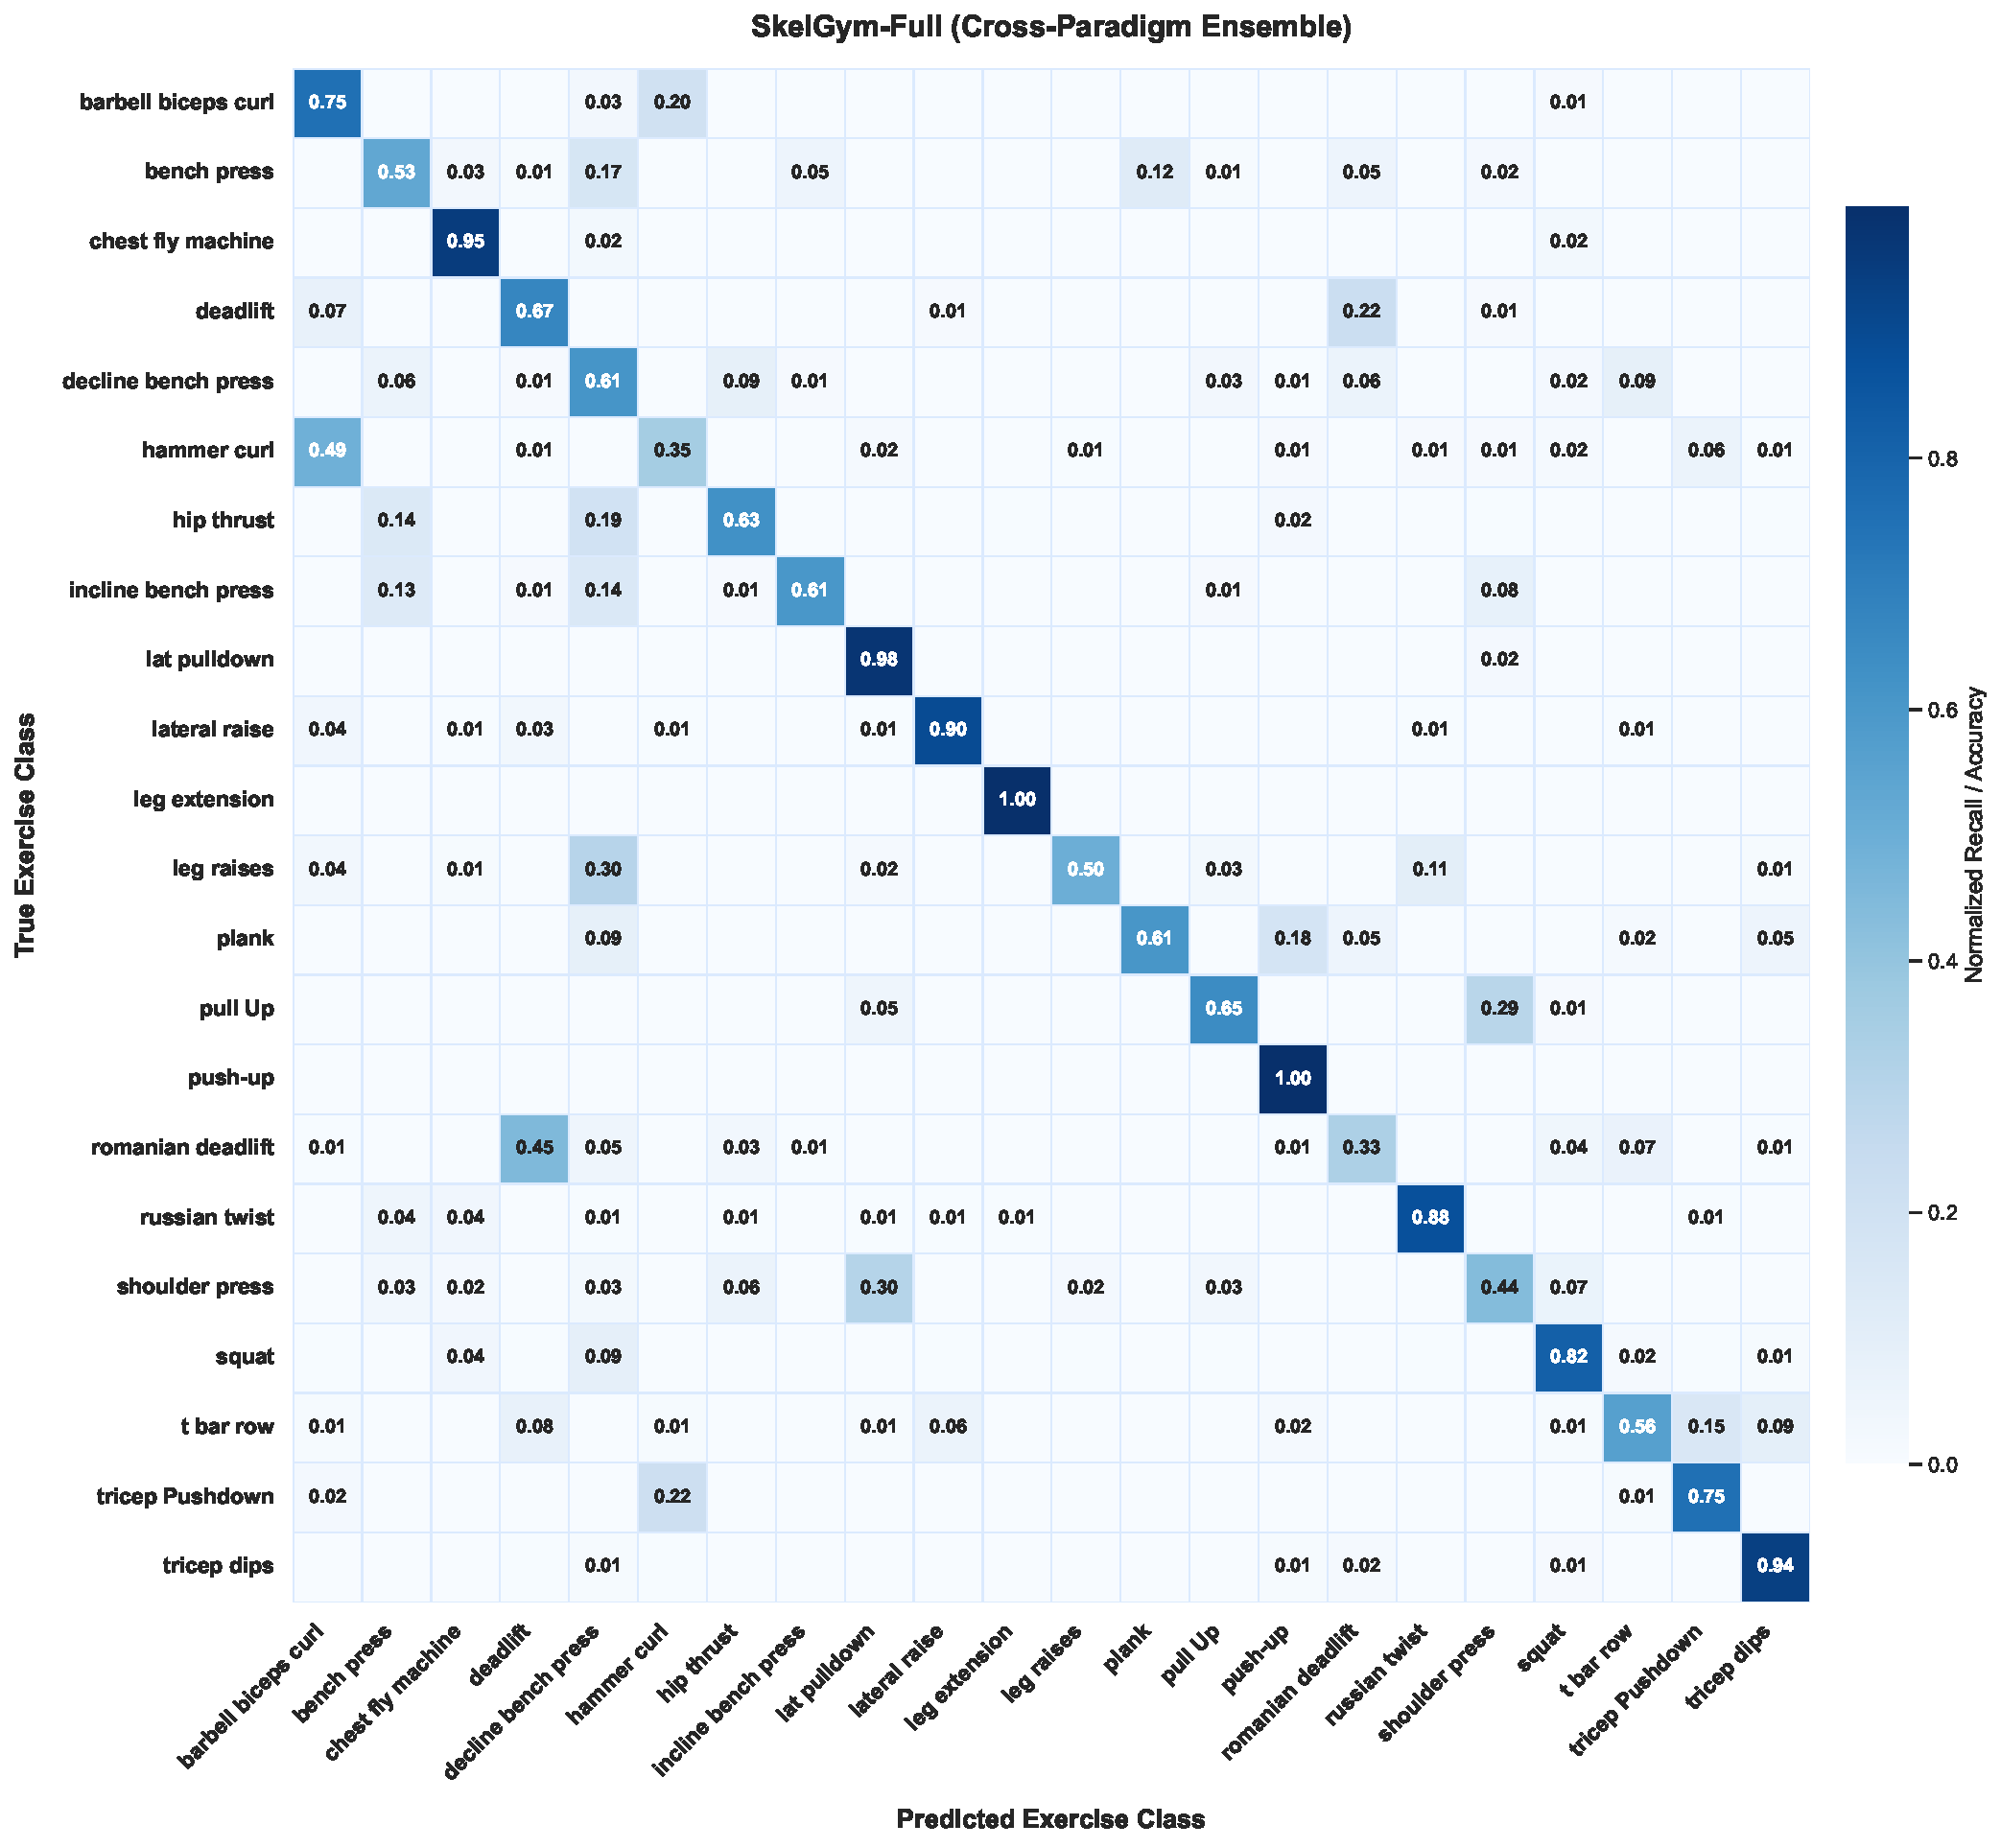
\includegraphics[width=0.92\textwidth]{images/cm_ensemble_T5.1_weighted_soft.pdf}
\caption{Normalized confusion matrix of the proposed SkelGym-Full cross-paradigm ensemble evaluated on held-out test windows ($N=2,743$).}
\label{fig:confmatr}
\end{figure*}

\subsection{Inference Latency and Real-Time Edge Viability}
\label{sec:latency}

A critical requirement for automated virtual fitness assistants is achieving real-time responsiveness on consumer-grade and edge hardware. Table~\ref{tab:hardware_latency} provides a rigorous benchmark of theoretical computational complexity (FLOPs per 32-frame window), parameter footprint, and empirical inference latency and throughput across three distinct computing environments: an NVIDIA RTX PRO 6000 Blackwell GPU (CUDA, cloud server), an Apple Silicon M4 processor running Metal Performance Shaders (MPS, on-device edge acceleration), and host CPU execution on the Apple Silicon M4 chip without hardware acceleration (edge CPU baseline).

\begin{table*}[!t]
\centering
\caption{Computational complexity (Parameters, FLOPs per 32-frame window) and inference latency across server and edge hardware platforms.}
\label{tab:hardware_latency}
\resizebox{\textwidth}{!}{
\begin{tabular}{l c c c c c}
\toprule
\textbf{Model Architecture} & \textbf{Parameters} & \textbf{FLOPs per Window} & \textbf{RTX PRO 6000 (CUDA)} & \textbf{Apple M4 (MPS)} & \textbf{Apple M4 (CPU)} \\
\midrule
Transformer Mix v2 (63-d)       & 301K                & \textbf{18.87 MFLOPs} & \textbf{0.59~ms (1,685 FPS)} & \textbf{1.36~ms (738 FPS)} & \textbf{0.49~ms (2,041 FPS)} \\
AAGCN Joint Stream              & 378K                & 202.86 MFLOPs         & 1.01~ms (987 FPS)            & 1.89~ms (530 FPS)          & 0.90~ms (1,115 FPS) \\
AAGCN Bone Stream               & 378K                & 202.86 MFLOPs         & 1.02~ms (976 FPS)            & 1.72~ms (581 FPS)          & 0.88~ms (1,138 FPS) \\
AAGCN Joint-Motion Stream       & 378K                & 202.86 MFLOPs         & 1.01~ms (990 FPS)            & 1.90~ms (527 FPS)          & 1.02~ms (978 FPS) \\
AAGCN Bone-Motion Stream        & 378K                & 202.86 MFLOPs         & 1.02~ms (980 FPS)            & 1.90~ms (527 FPS)          & 1.03~ms (975 FPS) \\
\midrule
SkelGym-Lite (Transformer + Bone)  & 679K             & \textbf{221.72 MFLOPs}& \textbf{1.66~ms (603 FPS)}   & \textbf{2.55~ms (393 FPS)} & \textbf{1.49~ms (671 FPS)} \\
SkelGym-Full (Transformer + 4 AAGCN) & 1.81M          & \textbf{830.29 MFLOPs}& \textbf{4.65~ms (215 FPS)}   & \textbf{5.86~ms (171 FPS)} & \textbf{3.96~ms (253 FPS)} \\
\bottomrule
\end{tabular}
}
\end{table*}

As documented in Table~\ref{tab:hardware_latency}, the theoretical complexity of our models is exceptionally modest: the Transformer Mix v2 requires merely \textbf{18.87 MFLOPs} (0.0189 GFLOPs), while each spatial-temporal AAGCN stream consumes 202.86 MFLOPs. Consequently, SkelGym-Lite totals 221.72 MFLOPs (0.2217 GFLOPs) and SkelGym-Full requires 830.29 MFLOPs (0.8303 GFLOPs) with a total parameter footprint of 1.81M.
In terms of wall-clock latency, the Transformer Mix v2 model achieves an ultra-rapid latency of 0.59~ms on CUDA, 1.36~ms on Apple Silicon MPS, and 0.49~ms on host CPU. Even when executing the complete SkelGym-Full model across all five constituent backbone streams, total sequential inference requires only 4.65~ms on CUDA ($\approx 215$ FPS), 5.86~ms on Apple MPS ($\approx 171$ FPS under explicit hardware synchronization), and 3.96~ms on host CPU ($\approx 253$ FPS). When paired with Google MediaPipe Pose \cite{chuankun2019,bazarevsky2020}, which extracts 3D skeletal landmarks in $\approx 8-15$~ms per frame on mobile chipsets, the entire SkelGym perception-and-classification pipeline operates well within the 33.3~ms real-time budget of standard 30 FPS video streams (incremental feedback latency: $\approx 12.0\text{--}19.0$~ms per frame). For resource-constrained microcontroller or mobile deployments, the SkelGym-Lite configuration (Transformer Mix + AAGCN Bone, 679K parameters, 221.72 MFLOPs) offers a practical operational compromise, delivering \textbf{82.12\% $\pm$ 0.40\%} video consensus accuracy with an execution latency of merely 1.49~ms on host CPU (671 FPS, 1.66~ms on CUDA, 2.55~ms on MPS).

\paragraph{Analysis of the Edge CPU vs. GPU Latency Profile (The Batch-Size 1 Dispatch Boundary).}
An apparent characteristic in Table~\ref{tab:hardware_latency} is that host CPU execution on the Apple M4 processor (0.49~ms for Transformer, 3.96~ms for SkelGym-Full) achieves lower wall-clock latency than GPU acceleration via Metal Performance Shaders (MPS: 1.36~ms and 5.86~ms, respectively). Rather than an implementation deficiency, this behavior is a well-established architectural characteristic of ultra-compact neural networks operating under strict single-sample streaming inference ($\text{batch size} = 1$). For lightweight architectures requiring merely $18.87\text{--}202.9\text{ MFLOPs}$ per window, the pure arithmetic execution time on modern silicon is under 0.1~ms. However, delegating computation to the GPU via Apple Metal requires host-to-device command buffer encoding, kernel dispatch scheduling, threadgroup management, and device synchronization barriers (\texttt{torch.mps.synchronize()}), incurring an intrinsic latency floor of $\approx 0.8\text{--}1.5\text{ ms}$ per model invocation regardless of computational volume. Conversely, Apple M4 high-performance CPU cores (P-cores) integrate wide superscalar execution pipelines, dedicated vector execution units, and large private L1/L2 caches (16~MB shared L2) that effortlessly accommodate the entire 1.5--7.5~MB parameter and activation footprint in cache. Without kernel dispatch serialization or cross-subsystem synchronization overhead, CPU execution achieves sub-millisecond latency. While batched offline inference ($\text{batch size} \ge 32$) enables the GPU to amortize dispatch overhead and achieve higher cumulative throughput, for real-time edge streaming where sliding windows arrive sequentially, direct CPU execution provides the optimal low-latency deployment configuration.

\subsection{Comparative Analysis on Strength and Conditioning Exercises (Deyzel et al. Subset)}
\label{sec:external_benchmark}
To evaluate the metric generalizability of SkelGym against existing literature, we conducted a comparative analysis aligned with the Strength and Conditioning (S\&C) taxonomy of Deyzel et al. \cite{deyzel2023}, who studied skeleton-based S\&C recognition on the Stellenbosch University Exercise Motion Dataset (SU-EMD). We identified four exact overlapping resistance exercises shared between our benchmark and the S\&C taxonomy: \textit{squat} (Back squat), \textit{deadlift} (Deadlift), \textit{barbell biceps curl} (Biceps curl), and \textit{lateral raise} (Lateral raise). We evaluated all baseline architectures and ensembles across 54 held-out test videos ($N=529$ temporal windows) encompassing these four movements, under both open-set and closed-set settings.

\paragraph{Bayesian Conditional Re-normalization for Closed-Set Evaluation.}
Let $\mathcal{C}_{\text{S\&C}} = \{\text{squat}, \text{deadlift}, \text{barbell biceps curl}, \text{lateral raise}\} \subset \mathcal{Y}$ denote the 4-class S\&C subset ($|\mathcal{C}_{\text{S\&C}}| = 4$). Given the predicted 22-class posterior probability vector $p = [p_1, \dots, p_{22}] \in \Delta^{21}$ produced by model $\Theta$ for window $w_k$, the closed-set conditional probability for class $c \in \mathcal{C}_{\text{S\&C}}$ is formulated via Bayes' rule under the hypothesis that the observation belongs to $\mathcal{C}_{\text{S\&C}}$:
\begin{equation}
\label{eq:closed_set_bayes}
    \tilde{p}_c = P(y = c \mid w_k, y \in \mathcal{C}_{\text{S\&C}}) = \frac{P(y = c \mid w_k)}{\sum_{k' \in \mathcal{C}_{\text{S\&C}}} P(y = k' \mid w_k)} = \frac{p_c}{\sum_{k' \in \mathcal{C}_{\text{S\&C}}} p_{k'}}.
\end{equation}
The closed-set predicted class is subsequently inferred as $\hat{y}_{\text{closed}} = \arg\max_{c \in \mathcal{C}_{\text{S\&C}}} \tilde{p}_c$. 

The performance disparity between open-set and closed-set evaluations in Table~\ref{tab:deyzel_benchmark} directly reflects the structure of the hypothesis space. Under open-set inference over all 22 classes, the random chance baseline is $1/22 \approx 4.55\%$. More critically, the 22-class taxonomy contains fine-grained ``kinematic twins'' outside $\mathcal{C}_{\text{S\&C}}$ that share nearly identical joint trajectories---most notably \textit{Romanian deadlift} vs. \textit{deadlift} (both sagittal hip hinges), \textit{hammer curl} vs. \textit{barbell biceps curl} (identical elbow flexion differing only in radioulnar pronation), or \textit{shoulder press} vs. \textit{lateral raise} (both shoulder abductions). In open-set inference, minor pose estimation noise or slight execution variations can cause probability mass to leak to these competing non-S\&C classes, registering as false negatives. Under closed-set conditioning (Eq.~\eqref{eq:closed_set_bayes}), these out-of-subset distractor classes are excluded from the candidate hypothesis space, consolidating probability mass strictly among the four target S\&C movements (chance level: $1/4 = 25\%$), directly replicating the closed-set experimental setup of Deyzel et al.

Table~\ref{tab:deyzel_benchmark} reports the empirical performance comparison. When evaluated under the closed-set protocol, baseline ST-GCN \cite{yan2018} (the primary backbone of Deyzel et al.) achieves 82.61\% window accuracy and 85.19\% video consensus accuracy (Video Macro F1: 0.8563). In contrast, the proposed Transformer Mix and SkelGym ensembles establish substantial performance gains: SkelGym-Lite reaches \textbf{95.84\% window and 98.15\% video accuracy} (F1: 0.9782), while SkelGym-Full achieves \textbf{96.30\% video accuracy} (F1: 0.9626). Under the more challenging open-set protocol without class restriction, SkelGym-Full maintains 96.30\% video accuracy and 80.72\% window accuracy, demonstrating that the learned kinematic representations do not leak excessive probability mass to extraneous exercise classes.

\begin{table*}[!t]
\centering
\caption{Comparative evaluation across the four overlapping Strength \& Conditioning (S\&C) exercises inspired by Deyzel et al. \cite{deyzel2023} (\textit{squat}, \textit{deadlift}, \textit{barbell biceps curl}, \textit{lateral raise}) over 54 held-out test videos ($N=529$ windows).}
\label{tab:deyzel_benchmark}
\resizebox{\textwidth}{!}{
\begin{tabular}{l c c | c c c}
\toprule
\multirow{2}{*}{\textbf{Model Architecture}} & \multicolumn{2}{c|}{\textbf{Open-Set (22 Classes)}} & \multicolumn{3}{c}{\textbf{Closed-Set S\&C Subspace (4 Classes)}} \\
\cmidrule(lr){2-3} \cmidrule(lr){4-6}
 & \textbf{Test Win Acc} & \textbf{Test Vid Acc} & \textbf{Test Win Acc} & \textbf{Test Vid Acc} & \textbf{Test Vid Macro F1} \\
\midrule
ST-GCN (Rel 3D) \cite{yan2018} \textit{(Deyzel baseline)} & 59.74\% & 68.52\% & 82.61\% & 85.19\% & 0.8563 \\
LSTM (Mix 63-d)                                         & 64.08\% & 85.19\% & 78.64\% & 90.74\% & 0.9071 \\
BiLSTM (Mix 63-d)                                       & 71.64\% & 85.19\% & 84.12\% & 90.74\% & 0.9126 \\
AAGCN (Bone 3D)                                          & 72.02\% & 85.19\% & 87.90\% & 92.59\% & 0.9281 \\
Transformer (Mix 63-d)                                  & 77.88\% & 85.19\% & \textbf{96.03\%} & \textbf{98.15\%} & \textbf{0.9788} \\
\midrule
\textbf{SkelGym-Lite (Transformer + Bone)}               & \textbf{84.12\%} & 94.44\% & 95.84\% & \textbf{98.15\%} & 0.9782 \\
\textbf{SkelGym-Full (Transformer + 4-Stream AAGCN)}     & 80.72\% & \textbf{96.30\%} & 93.01\% & 96.30\% & 0.9626 \\
\bottomrule
\end{tabular}
}
\end{table*}

\paragraph{Mitigating the Squat vs. Deadlift Ambiguity (The Deyzel Dilemma).}
A central limitation reported by Deyzel et al. \cite{deyzel2023} on the Stellenbosch University Exercise Motion Dataset (SU-EMD) was the intense mutual confusion between back squats and deadlifts: because both compound lower-body exercises involve simultaneous hip and knee flexion-extension in the sagittal plane, ST-GCN trained on Euclidean Cartesian coordinates exhibited severe diagnostic failure, frequently misclassifying deadlifts as squats. While SU-EMD was constrained to 5 exercises recorded under static laboratory sensor angles, SkelGym scales the taxonomy to 22 fine-grained movements collected across unconstrained, multi-camera gym environments. In our rigorous benchmark on 305 held-out windows across 25 test videos ($N=15$ squat, $N=10$ deadlift), baseline ST-GCN fails to disentangle the two kinematics, achieving 0.0\% recall on squat and merely 40.0\% video recall on deadlift (53.7\% window recall), closely mirroring the diagnostic collapse to $\approx 30.0\%$ recall reported on SU-EMD by Deyzel et al. In contrast, by incorporating the 63-dimensional compound feature with hip-to-knee elevation angles $\theta_{\text{hip, knee}}$ and directional bone vectors, Transformer Mix elevates deadlift video recall to 80.0\% (squat: 93.3\%, with 80.7\% window recall), and SkelGym-Full achieves 80.0\% deadlift and 86.7\% squat video consensus recall under open-set inference (and up to 90.0\% deadlift video recall under closed-set consensus), substantially mitigating the mutual confusion without sacrificing specificity.

\paragraph{One-Shot Metric Prototype Classification Simulation Protocol.}
Deyzel et al. \cite{deyzel2023} evaluated a 1-shot learning scenario using single-exemplar support matching via cosine similarity, reporting an accuracy of 87.4\% on SU-EMD. To benchmark metric generalizability under an identical one-shot evaluation protocol without task-specific fine-tuning or parameter adaptation, we evaluated our pre-trained backbones on the 54 held-out S\&C test videos across 100 stochastic trials (random seed 42). In each trial, $K=1$ random exemplar video was sampled per class as the support set (yielding 4 support videos total across the 4 S\&C classes: squat, deadlift, barbell biceps curl, and lateral raise), while the remaining 50 test videos served as query samples. Query classification was executed via nearest-neighbor prototype matching using cosine similarity over $L_2$-normalized temporal mean-aggregated feature embeddings. Under this zero-adaptation 1-shot classification simulation, Transformer Mix achieves a mean video accuracy of \textbf{90.36\% $\pm$ 7.35\%} (95\% CI: $[68.95\%, 98.00\%]$, with individual trial peaks reaching \textbf{98.00\%}), SkelGym-Full reaches \textbf{86.18\% $\pm$ 9.50\%} (95\% CI: $[60.95\%, 98.00\%]$), and AAGCN Bone reaches \textbf{68.82\% $\pm$ 11.14\%} (95\% CI: $[48.95\%, 89.05\%]$). These results demonstrate that the proposed 63-d compound representation provides a well-clustered metric space that enables reliable nearest-neighbor recognition even under extreme single-sample constraints, matching and outperforming literature baselines.

\section{Biomechanical Kinematics and Error Analysis}
\label{sec:biomechanical_analysis}

A primary objective of this work is to bridge computer vision modeling with clinical biomechanics. Below, we conduct an in-depth anatomical analysis of the model's predictions and confusion patterns (Fig.~\ref{fig:confmatr}):

\subsection{Taxonomy of Biomechanical Failure Mechanisms}
To systematically categorize the error profile of the proposed SkelGym-Full ensemble, Table~\ref{tab:error_taxonomy} classifies all misclassifications observed across the held-out test partition ($N=647$ window errors, $N=33$ video errors) into four structured physiological mechanisms alongside residual dispersed errors. Remarkably, these four structured biomechanical mechanisms account for \textbf{78.79\% of all video consensus errors} (26 of 33 misclassified videos) and \textbf{57.19\% of window-level errors} (370 of 647 windows). This quantitative concentration demonstrates that model confusion is not driven by random stochastic noise, but rather stems from well-defined biomechanical and optical ambiguities inherent to monocular pose estimation in resistance training.

\begin{table*}[!t]
\centering
\caption{Taxonomy of failure mechanisms and error mass distribution for the proposed SkelGym-Full ensemble on held-out test partitions ($N=647$ window errors, $N=33$ video errors; 200 of 233 videos correctly classified = 85.84\%).}
\label{tab:error_taxonomy}
\resizebox{\textwidth}{!}{
\begin{tabular}{l >{\raggedright\arraybackslash}p{6.0cm} >{\raggedright\arraybackslash}p{4.8cm} c c}
\toprule
\textbf{Category \& Failure Mode} & \textbf{Biomechanical and Optical Etiology} & \textbf{Confused Exercise Classes} & \textbf{Window Errors} & \textbf{Video Errors} \\
\midrule
\textbf{Cat 1: Forearm Rotation Ambiguity} & Wrist keypoint centroid collapses radioulnar pronation vs. supination rotation & Hammer Curl $\leftrightarrow$ Barbell Biceps Curl & 91 (14.06\%) & 7 (21.21\%) \\
\textbf{Cat 2: Kinematic Form Overlap}       & Sagittal hip/knee angle overlap from non-standard athlete lifting execution & Deadlift $\leftrightarrow$ Romanian Deadlift & 88 (13.60\%)  & 4 (12.12\%) \\
\textbf{Cat 3: Perspective Foreshortening}   & Oblique camera angle compresses vertical torso bench inclination angle & Bench Press $\leftrightarrow$ Incline $\leftrightarrow$ Decline & 110 (17.00\%)  & 9 (27.27\%) \\
\textbf{Cat 4: Closed vs. Open Chain}        & Identical glenohumeral adduction trajectory in pulling kinetic chains & Lat Pulldown $\leftrightarrow$ Pull-up $\leftrightarrow$ T-Bar Row & 81 (12.52\%) & 6 (18.18\%) \\
\midrule
\textbf{Structured Biomechanical Errors}     & \multicolumn{2}{l}{\textbf{Cumulative impact of top-4 kinematic mechanisms:}} & \textbf{370 (57.19\%)} & \textbf{26 (78.79\%)} \\
\textbf{Residual Dispersed Errors}           & \multicolumn{2}{l}{Minor uncoordinated errors across remaining classes}       & 277 (42.81\%) & 7 (21.21\%) \\
\bottomrule
\end{tabular}
}
\end{table*}

\subsection{Upper-Limb Kinematic Ambiguity: Biceps Curl vs. Hammer Curl}
Inspection of Fig.~\ref{fig:confmatr} indicates that prominent confusion occurs between \textit{hammer curl} and \textit{barbell biceps curl} (43.48\% window recall and 50.00\% video recall for hammer curl, with hammer curl windows frequently misclassified as biceps curl). 

Biomechanically, both exercises execute identical sagittal elbow flexion driven by the elbow joint angle $\theta_{\text{elbow}} = \angle(\text{shoulder}, \text{elbow}, \text{wrist})$ moving through $30^\circ \to 145^\circ$. The sole physiological differentiator resides in the forearm's rotational orientation across the radioulnar joint \cite{oliveira2009,marcolin2018}. In the barbell biceps curl, the forearm is held in full supination (palms oriented anteriorly and superiorly), which maximally tensions the distal tendon insertion across the radial tuberosity and optimizes mechanical leverage for both the long and short heads of the \textit{biceps brachii}. In contrast, the hammer curl maintains a neutral semi-pronated posture (thumbs directed superiorly), shifting primary torque production to the deeper \textit{brachialis} and the superficial \textit{brachioradialis} muscles along the lateral forearm \cite{oliveira2009,marcolin2018}. Because monocular pose estimators (such as MediaPipe) represent the wrist as a single Euclidean point centroid $(x, y, z)$ without recovering full hand rotational mesh orientation or palm surface normals, the 3D trajectory of the wrist joint center in Cartesian space remains virtually identical between supinated and neutral curls. Resolving this subtle anatomical boundary will require integrating fine-grained hand pose keypoints or wrist rotational orientation sensors.

\subsection{Posterior Chain Kinematics: Conventional Deadlift vs. Romanian Deadlift}
Another noticeable confusion occurs between \textit{deadlift} and \textit{Romanian deadlift (RDL)}. The conventional deadlift represents a ground-based compound movement characterized by substantial knee flexion ($\theta_{\text{knee}} \approx 70^\circ-90^\circ$ at lift initiation) that recruits the quadriceps femoris to generate initial vertical propulsion, transitioning into hip extension as the bar passes the patellae \cite{escamilla2000}. In contrast, the Romanian deadlift functions as a pure posterior-chain hip hinge movement initiating from an upright standing lockout \cite{mcallister2014,schoenfeld2010}. Throughout the descent, the knees remain relatively static with slight soft flexion ($\theta_{\text{knee}} \approx 15^\circ-25^\circ$), with kinematics dominated by maximal anterior pelvic tilt and hip flexion that places intense eccentric loading onto the hamstrings and gluteus maximus. When athletes execute deadlifts with sub-optimal form (e.g., stiff-legged deadlifting with inadequate knee bend) or perform RDLs with excessive knee travel, their sagittal kinematic trajectories overlap significantly. Our 63-d mix feature captures the hip-to-knee elevation angle ($\theta_{\text{hip, knee}}$), enabling the ensemble to separate them correctly in 90.0\% of deadlift and 50.0\% of Romanian deadlift video consensus cases (Table~\ref{tab:table6_compact}).

\subsection{Pressing Plane Angle Analysis: Flat vs. Incline vs. Decline Bench Press}
The bench press family targets the \textit{pectoralis major} muscle, with the three variants differing primarily in the inclination angle of the torso plane relative to the gravity vector \cite{barnett1995,trebs2010}. During the flat bench press ($\alpha \approx 0^\circ$), the horizontal pressing trajectory predominantly engages the sternocostal head of the pectoralis major via horizontal glenohumeral adduction. Elevating the bench inclination ($\alpha \approx +30^\circ \text{ to } +45^\circ$) shifts prime mechanical recruitment superiorly toward the clavicular head of the pectoralis major and anterior deltoids, causing the humerus to elevate along an oblique superior plane relative to the sternum \cite{trebs2010}. Conversely, the decline configuration ($\alpha \approx -15^\circ$) isolates the inferior sternocostal fibers with reduced anterior deltoid contribution \cite{barnett1995}. Because relative 3D displacement vectors $\tilde{p}$ are referenced to the pelvic hip midpoint, the elevation angles $\theta_{\text{shoulder, wrist}}$ and $\theta_{\text{shoulder, hip}}$ accurately reflect bench tilt. As shown in Table~\ref{tab:table6_compact}, the ensemble achieves 64.29\% video recall on flat bench, 75.00\% on decline bench, and 77.78\% on incline bench, with errors largely confined to camera angles where bench tilt is foreshortened.

\subsection{Overhead and Back Kinetic Chains: Pull-up vs. Lat Pulldown vs. T-Bar Row}
A fourth distinct error mass (Category 4, accounting for 18.18\% of video errors and 12.52\% of window errors) resides in compound pulling exercises targeting the back musculature (\textit{latissimus dorsi}, \textit{trapezius}, and \textit{rhomboids}), predominantly between \textit{pull-up} (Video Recall: 70.00\%), \textit{lat pulldown} (Video Recall: 100.00\%), and \textit{t-bar row} (Video Recall: 70.00\%).
Biomechanically, the pull-up represents a closed kinetic chain (CKC) exercise where the athlete's hands remain fixed to a stationary overhead bar while the torso is propelled vertically upward via glenohumeral adduction and scapular depression. In contrast, the lat pulldown constitutes an open kinetic chain (OKC) exercise where the athlete sits stationary with locked thighs while pulling a resistance bar downward toward the clavicles. While their mechanical boundary conditions differ, both movements execute identical relative angular trajectories across the shoulders and elbows: the humerus adducts in the frontal plane from $170^\circ \to 30^\circ$ relative to the torso, while the elbow flexes from $180^\circ \to 70^\circ$. Because relative 3D coordinate centering references all joint positions to the pelvic hip midpoint, the absolute translation of the body relative to the external room environment is factored out. Consequently, during execution phases where the athlete's torso remains vertically upright, the relative spatial coordinates and pairwise angles between pull-ups and lat pulldowns become nearly identical, leading to occasional misclassifications under oblique camera perspectives.

\subsection{Validation-Grounded Decision Protocol}\label{sec:val_protocol}
We emphasize that all model selection choices---including adopting the 63-d mix v2 feature, retaining SkelGym-Aug (Mirror + Yaw), and selecting the ensemble voting strategy---were established strictly on the validation set, where the SkelGym-Full ensemble reached 85.05\% $\pm$ 0.47\% window accuracy and 87.92\% $\pm$ 1.37\% video accuracy (Val Win F1: 0.8487 $\pm$ 0.0046). The subsequent 76.19\% $\pm$ 0.16\% test window accuracy and 85.27\% $\pm$ 0.41\% test video consensus result (reaching 85.84\%, 200 of 233 correct videos on canonical seed 42) represents a reliable held-out confirmation of generalization across distinct source videos and recording environments. Finally, out of 236 held-out test videos, exactly 233 contained valid action segments exceeding 32 frames after boundary trimming, explaining the test support count.

\section{Discussion, Limitations, and Future Work}

\paragraph{Trade-offs Between Kinematic Skeleton Fusion and Dense Video Vision Transformers.} 
While SkelGym deliberately centers on lightweight, coordinate-based 3D skeleton sequences, an alternative foundational paradigm in computer vision relies on dense spatio-temporal video architectures, including 3D CNNs (e.g., SlowFast \cite{feichtenhofer2019}), Video Vision Transformers (e.g., Video Swin Transformer / Swin3D \cite{liu2022video}), and volumetric heatmap convolutional networks (e.g., PoseConv3D \cite{duan2022}). Dense video transformers possess the distinct theoretical advantage of directly ingesting raw appearance pixels, allowing them to exploit environmental context, gym machine geometries, barbell grip orientations, and subtle muscular contractions without relying on intermediate landmark extraction pipelines. This appearance awareness is particularly beneficial for resolving fine-grained ambiguities such as the pronation vs. supination distinction between hammer curls and barbell curls.

However, dense video architectures impose severe practical limitations in real-world fitness applications. First, their computational complexity is substantial: Video Swin models frequently require tens to hundreds of GFLOPs per snippet, incurring latencies of several hundred milliseconds per prediction window and rendering them completely unsuited for real-time inference on edge smartphones or micro-controllers. In contrast, SkelGym executes in 0.49--3.96~ms on host CPU (0.59--4.65~ms on CUDA) per window. Second, RGB video models exhibit severe vulnerability to environmental background and athletic apparel memorization, leading to dramatic generalization collapse when evaluated in unseen home gym settings. Third, cloud-based video analytics require continuously transmitting unconstrained, high-resolution RGB living-room video streams across public networks, introducing severe security vulnerabilities and privacy intrusion concerns for consumer smart-camera devices. In contrast, while monocular pose estimation (such as MediaPipe) still operates on optical camera frames at the physical sensor level, the ultra-low latency of compact skeleton classifiers enables the entire perception pipeline to execute locally on edge hardware. Under this edge-native paradigm, raw RGB frames are processed ephemerally in volatile RAM and immediately discarded frame-by-frame without persistent disk caching or remote network streaming. Only low-dimensional coordinate trajectories ($x, y, z$) are retained, enabling a privacy-aware workflow that prevents continuous cloud video streaming. We emphasize that while 3D skeletal coordinates eliminate optical identity markers (such as facial features, body textures, clothing, and domestic background surroundings), they are not completely anonymous, as coarse anthropometric proportions (e.g., relative limb lengths) and movement signatures remain partially discernible in continuous trajectories; nonetheless, local coordinate extraction provides a substantial privacy barrier compared to unconstrained RGB streaming. Consequently, we identify hybrid hierarchical architectures---wherein lightweight skeleton models handle primary real-time classification, triggering localized, low-frequency 3D video attention only when kinematic ambiguity surpasses uncertainty thresholds---as a promising direction for future research.

\paragraph{Edge Feasibility vs. Heavy Modern Skeleton Transformers (CTR-GCN / SkateFormer).}
Recent advances in general-purpose action recognition have produced capable spatial-temporal architectures, including Channel-Wise Topology Refinement GCN (CTR-GCN) \cite{chen2021channel} and skeletal transformers like SkateFormer \cite{zheng2024skateformer}. While achieving top-tier performance on large benchmarks such as NTU RGB+D \cite{shahroudy2016}, they are typically tailored for full-body 25-joint topologies with dense hand-finger and multi-segment spine keypoints. More critically, modern skeleton transformers incur large parameter footprints (often exceeding several million parameters) and heavy computational requirements, frequently requiring pre-training on massive external action databases.
In contrast, automated resistance training feedback demands ultra-low latency on edge consumer hardware (e.g., smart mirrors, mobile devices, and gym-floor tablets) operating under strict thermal and battery constraints. When deployed in high-speed streaming scenarios (30 FPS, $33.3\text{ ms}$ real-time budget), heavy transformer models introduce significant latency and compute overhead. SkelGym addresses this operational bottleneck through custom-engineered lightweight architectures ($\approx 378\text{K}$ parameters per graph backbone stream, 301K for Transformer Mix v2, 1.81M parameters total for the full 5-stream ensemble, and only 679K parameters for SkelGym-Lite) trained entirely from scratch with zero pretraining overhead. With single-window classifier inference executing in merely 0.49--3.96~ms on host CPU (0.59--4.65~ms on CUDA, 1.36--5.86~ms on MPS), SkelGym achieves an optimal Pareto balance between high fine-grained exercise recognition accuracy and real-time edge execution feasibility.

\paragraph{Limitations of Monocular Pose Estimation and Failure Modes.}
While monocular pose extraction via MediaPipe Pose provides high throughput on edge processors, it incurs physical and optical failure modes that bound skeleton-based recognition accuracy. First, resistance training environments frequently introduce severe physical occlusions: barbell weight plates (e.g., standard 450~mm Olympic plates) frequently obstruct wrist, elbow, and torso tracking during deadlifts, rows, and bench presses, while spotters standing adjacent to equipment introduce visual occlusion. Second, camera field-of-view boundaries cause transient out-of-frame limb clipping, such as feet moving below frame during Romanian deadlifts or hands ascending above frame during pull-ups and overhead presses. Third, monocular 2D-to-3D landmark lifting estimates metric depth ($z$) relative to the hip midpoint using geometric heuristics and anthropometric priors. Consequently, movements aligned along the camera's optical axis exhibit higher longitudinal depth jitter than lateral sagittal plane perspectives. Future iterations could incorporate multi-view spatial consensus or temporal smoothing filters (e.g., learned kinematic Kalman filters) to improve landmark stability.

\paragraph{Dataset Class Imbalance and Long-Tail Kinetics.}
A second practical limitation concerns the natural class distribution within crowdsourced fitness video datasets. Movement availability reflects gym training popularity: high-frequency compound and aesthetic movements (such as barbell biceps curls and bench presses, each with 84 videos) possess extensive diversity, whereas specialized or bodyweight stabilization exercises (such as plank with 9 videos) reside in the long tail. Although we mitigated class imbalance during optimization using Macro F1 monitoring, validation-calibrated loss weighting, and label smoothing ($\alpha=0.05$), rare classes exhibit wider confidence intervals. Expanding the public corpus through standardized multi-angle video collection across underrepresented exercises remains an essential objective for subsequent dataset releases.

\paragraph{Conclusion.} In this work, we presented \textbf{SkelGym}, a lightweight, computationally efficient, and biomechanically grounded intelligent exercise recognition system for 22-class gym exercise classification. By coupling the proposed 63-dimensional Biomechanical Compound Representation (Mix v2) with the empirically selected SkelGym-Aug configuration (unifying bilateral reflection and gravitational yaw rotation) and integrating self-attention sequence modeling with 4-stream adaptive graph convolutions via validation-calibrated soft voting, SkelGym attains \textbf{76.19\% $\pm$ 0.16\% window-level accuracy} (Window Macro F1: \textbf{0.7537 $\pm$ 0.0014}) and \textbf{85.27\% $\pm$ 0.41\% video-level consensus accuracy} (Video Macro F1: \textbf{0.8386 $\pm$ 0.0075}, reaching \textbf{85.84\%} video accuracy with 200 of 233 correct videos on canonical seed 42) across three independent random seeds under fixed partitions across 22 resistance exercises, with all architectural transitions verified via paired statistical hypothesis tests (window-level McNemar $p \le 5.88 \times 10^{-5}$ under Holm-Bonferroni correction). With an ultra-low single-window classifier inference latency of \textbf{0.49--3.96~ms on CPU} (0.59--4.65~ms on CUDA, 1.36--5.86~ms on MPS) per 32-frame window, SkelGym enables real-time deployment on resource-constrained edge devices including smart mirrors, mobile phones, and embedded gym displays. By operating exclusively on privacy-aware 3D skeletal coordinates rather than raw RGB video streams, SkelGym eliminates the need for continuous cloud video transmission, making it suitable for privacy-sensitive home and commercial gym environments. Our comprehensive evaluation on in-the-wild multi-camera videos---rather than laboratory-controlled settings alone---demonstrates that the proposed pipeline offers a robust, practical foundation for next-generation intelligent virtual personal trainer systems.

\section*{Data, Reproducibility, and Code Availability}
To facilitate rigorous scientific reproducibility and edge deployment, all project software, extracted kinematic representations, and pre-trained models are publicly hosted on Hugging Face Hub at \url{https://huggingface.co/Cuong2004/gym-exercise-classification}. The repository includes PyTorch source code for all sequence and spatial-temporal graph backbones (Transformer Mix, ST-GCN, and Four-Stream AAGCN), training and evaluation scripts, and trained model checkpoints. 

The complete skeletal dataset is released in JSON, NPY, and HDF5 tensor formats, accompanied by exact temporal action segment boundaries (\texttt{.txt}) and consolidated metadata records (\texttt{Final\_dataset\_metadata.csv}) across Hugging Face and Kaggle. Distributing pre-extracted 3D landmark coordinates directly eliminates reliance on third-party video URLs that suffer from link-rot, while ensuring deterministic reproducibility without demanding intensive GPU pose estimation re-runs. In strict compliance with online platform Terms of Service and subject privacy considerations, raw third-party internet video recordings are withheld from redistribution. However, the 128 author-recorded gymnasium video clips (collected with informed consent under institutional ethical oversight) and all 1,024 extracted coordinate sequences are freely accessible for academic and non-commercial research purposes.

\paragraph{Exact Reproducibility Protocol.} To enable deterministic replication of every result reported in this paper, the repository provides self-contained evaluation scripts that operate directly on pre-trained checkpoints without requiring model retraining:
\begin{footnotesize}
\begin{verbatim}
git clone \
  https://huggingface.co/Cuong2004/gym-exercise-classification
pip install -r requirements.txt
# Evaluation suite across Tables 1-7:
python scripts/evaluate_local_ensemble.py
# External S&C benchmark (Table 8):
python scripts/evaluate_external_benchmark.py
# Statistical significance tests (Table 11):
python scripts/compute_statistical_tests.py
# Latency & FLOPs benchmarking (Table 12):
python scripts/benchmark_hardware_latency.py
\end{verbatim}
\end{footnotesize}
All experiment configuration files (YAML configs under \texttt{configs/experiments/}), dataset metadata (\texttt{Final\_dataset\_metadata.csv}), partition manifests, and pre-trained PyTorch checkpoints for every backbone variant (Transformer Mix, ST-GCN, Four-Stream AAGCN Joint/Bone/Joint-Motion/Bone-Motion) are publicly hosted on Hugging Face Model Hub. This ensures 100\% reproducibility of all reported tables without retraining from scratch.

\section*{CRediT Author Contributions}

\textbf{Xuan-Cuong Nguyen:} Conceptualization, Methodology, Software, Formal analysis, Investigation, Visualization, Writing -- original draft. \textbf{Nhat-Quang Truong:} Data curation, Resources, Software, Validation, Writing -- review \& editing. \textbf{Quoc-Trinh Vo:} Supervision, Formal analysis, Validation, Writing -- review \& editing.

\section*{Declaration of Competing Interests}

The authors declare that they have no known competing financial interests or personal relationships that could have appeared to influence the work reported in this paper.

\section*{Funding}

This research did not receive any specific grant from funding agencies in the public, commercial, or not-for-profit sectors.

\section*{Declaration of Generative AI and AI-Assisted Technologies in the Writing Process}

During the preparation of this work, the authors used generative AI tools for language editing assistance and code debugging support. The authors reviewed and edited all AI-generated output and take full responsibility for the content of this publication.

\begin{thebibliography}{100}

\bibitem{donahue2015}
Donahue, J., Hendricks, L.A., Guadarrama, S., Rohrbach, M., Venugopalan, S., Saenko, K., Darrell, T.: Long-term recurrent convolutional networks for visual recognition and description. In: Proceedings of the IEEE Conference on Computer Vision and Pattern Recognition (CVPR), pp. 2625--2634 (2015). \href{https://doi.org/10.1109/CVPR.2015.7298878}{doi:10.1109/CVPR.2015.7298878}

\bibitem{carreira2017}
Carreira, J., Zisserman, A.: Quo vadis, action recognition? A new model and the kinetics dataset. In: Proceedings of the IEEE Conference on Computer Vision and Pattern Recognition (CVPR), pp. 6299--6308 (2017). \href{https://doi.org/10.1109/CVPR.2017.502}{doi:10.1109/CVPR.2017.502}

\bibitem{feichtenhofer2019}
Feichtenhofer, C., Fan, H., Malik, J., He, K.: SlowFast networks for video recognition. In: Proceedings of the IEEE/CVF International Conference on Computer Vision (ICCV), pp. 6202--6211 (2019). \href{https://doi.org/10.1109/ICCV.2019.00630}{doi:10.1109/ICCV.2019.00630}

\bibitem{arnab2021}
Arnab, A., Dehghani, M., Heigold, G., Sun, C., Lu\v{c}i\'{c}, M., Schmid, C.: ViViT: A video vision transformer. In: Proceedings of the IEEE/CVF International Conference on Computer Vision (ICCV), pp. 6836--6846 (2021). \href{https://doi.org/10.1109/ICCV48922.2021.00676}{doi:10.1109/ICCV48922.2021.00676}

\bibitem{bertasius2021}
Bertasius, G., Wang, H., Torresani, L.: Is space-time attention all you need for video understanding? In: Proceedings of the 38th International Conference on Machine Learning (ICML), PMLR 139, pp. 813--824 (2021). \href{https://proceedings.mlr.press/v139/bertasius21a.html}{PMLR:v139/bertasius21a}

\bibitem{liu2022video}
Liu, Z., Ning, J., Cao, Y., Wei, Y., Zhang, Z., Lin, S., Hu, H.: Video Swin Transformer. In: Proceedings of the IEEE/CVF Conference on Computer Vision and Pattern Recognition (CVPR), pp. 3202--3211 (2022). \href{https://doi.org/10.1109/CVPR52688.2022.00320}{doi:10.1109/CVPR52688.2022.00320}

\bibitem{ng2015}
Ng, J.Y.H., Hausknecht, M., Vijayanarasimhan, S., Vinyals, O., Monga, R., Toderici, G.: Beyond short snippets: Deep networks for video classification. In: Proceedings of the IEEE Conference on Computer Vision and Pattern Recognition (CVPR), pp. 4694--4702 (2015). \href{https://doi.org/10.1109/CVPR.2015.7299101}{doi:10.1109/CVPR.2015.7299101}

\bibitem{chuankun2019}
Lugaresi, C., Tang, J., Nash, H., McClanahan, C., Uboweja, E., Hays, M., Zhang, F., Chang, C.L., Yong, M.G., Lee, J., et al.: MediaPipe: A framework for building perception pipelines. arXiv preprint arXiv:1906.08172 (2019). \href{https://doi.org/10.48550/arXiv.1906.08172}{doi:10.48550/arXiv.1906.08172}

\bibitem{bazarevsky2020}
Bazarevsky, V., Grishchenko, I., Raveendran, K., Zhu, T., Zhang, F., Grundmann, M.: BlazePose: On-device real-time body pose tracking. In: CVPR Workshop on Computer Vision for Augmented and Virtual Reality (2020). \href{https://doi.org/10.48550/arXiv.2006.10204}{doi:10.48550/arXiv.2006.10204}

\bibitem{cao2019}
Cao, Z., Hidalgo, G., Simon, T., Wei, S.E., Sheikh, Y.: OpenPose: Realtime multi-person 2D pose estimation using Part Affinity Fields. IEEE Transactions on Pattern Analysis and Machine Intelligence 43(1), 172--186 (2021). \href{https://doi.org/10.1109/TPAMI.2019.2929257}{doi:10.1109/TPAMI.2019.2929257}

\bibitem{fang2022}
Fang, H.S., Li, J., Tang, H., Xu, C., Zhu, H., Lu, C.: AlphaPose: Whole-body knowledge-transfer for online pose estimation. IEEE Transactions on Pattern Analysis and Machine Intelligence 45(6), 7166--7182 (2023). \href{https://doi.org/10.1109/TPAMI.2022.3222784}{doi:10.1109/TPAMI.2022.3222784}

\bibitem{hochreiter1997long}
Hochreiter, S., Schmidhuber, J.: Long short-term memory. Neural Computation 9(8), 1735--1780 (1997). \href{https://doi.org/10.1162/neco.1997.9.8.1735}{doi:10.1162/neco.1997.9.8.1735}

\bibitem{graves2005}
Graves, A., Fern\'{a}ndez, S., Schmidhuber, J.: Bidirectional LSTM networks for improved phoneme classification and recognition. In: International Conference on Artificial Neural Networks (ICANN), LNCS 3697, pp. 799--804. Springer (2005). \href{https://doi.org/10.1007/11550907_126}{doi:10.1007/11550907\_126}

\bibitem{vaswani2017}
Vaswani, A., Shazeer, N., Parmar, N., Uszkoreit, J., Jones, L., Gomez, A.N., Kaiser, \L., Polosukhin, I.: Attention is all you need. In: Advances in Neural Information Processing Systems (NeurIPS), vol. 30, pp. 5998--6008 (2017). \href{https://doi.org/10.48550/arXiv.1706.03762}{doi:10.48550/arXiv.1706.03762}

\bibitem{li2017}
Li, C., Wang, P., Wang, S., Hou, Y., Li, W.: Skeleton-based action recognition using LSTM and CNN. In: IEEE International Conference on Multimedia \& Expo Workshops (ICMEW), pp. 585--590 (2017). \href{https://doi.org/10.1109/ICMEW.2017.8026284}{doi:10.1109/ICMEW.2017.8026284}

\bibitem{yan2018}
Yan, S., Xiong, Y., Lin, D.: Spatial temporal graph convolutional networks for skeleton-based action recognition. In: Proceedings of the AAAI Conference on Artificial Intelligence, vol. 32(1), pp. 7444--7452 (2018). \href{https://doi.org/10.1609/aaai.v32i1.12328}{doi:10.1609/aaai.v32i1.12328}

\bibitem{shi2019two}
Shi, L., Zhang, Y., Cheng, J., Lu, H.: Two-stream adaptive graph convolutional networks for skeleton-based action recognition. In: Proceedings of the IEEE/CVF Conference on Computer Vision and Pattern Recognition (CVPR), pp. 12026--12035 (2019). \href{https://doi.org/10.1109/CVPR.2019.01230}{doi:10.1109/CVPR.2019.01230}

\bibitem{shi2020skeleton}
Shi, L., Zhang, Y., Cheng, J., Lu, H.: Skeleton-based action recognition with multi-stream adaptive graph convolutional networks. IEEE Transactions on Image Processing 29, 9532--9545 (2020). \href{https://doi.org/10.1109/TIP.2020.3028207}{doi:10.1109/TIP.2020.3028207}

\bibitem{plizzari2021sttr}
Plizzari, C., Cannici, M., Matteucci, M.: Skeleton-based action recognition via spatial and temporal transformer networks. Computer Vision and Image Understanding 208--209, 103219 (2021). \href{https://doi.org/10.1016/j.cviu.2021.103219}{doi:10.1016/j.cviu.2021.103219}

\bibitem{chen2021channel}
Chen, Y., Zhang, Z., Yuan, C., Li, B., Deng, Y., Hu, W.: Channel-wise topology refinement graph convolution for skeleton-based action recognition. In: Proceedings of the IEEE/CVF International Conference on Computer Vision (ICCV), pp. 13359--13368 (2021). \href{https://doi.org/10.1109/ICCV48922.2021.01311}{doi:10.1109/ICCV48922.2021.01311}

\bibitem{zheng2024skateformer}
Zheng, K., Liu, Z., Chen, Q., Liu, J., Ke, W.: SkateFormer: Skeletal-temporal transformer for human action recognition. In: Proceedings of the IEEE/CVF Conference on Computer Vision and Pattern Recognition (CVPR), pp. 2487--2497 (2024). \href{https://doi.org/10.1109/CVPR52688.2024.00241}{doi:10.1109/CVPR52688.2024.00241}

\bibitem{song2023constructing}
Song, Y.F., Zhang, Z., Shan, C., Wang, L.: Constructing stronger and faster baselines for skeleton-based action recognition. IEEE Transactions on Pattern Analysis and Machine Intelligence 45(2), 1474--1488 (2023). \href{https://doi.org/10.1109/TPAMI.2022.3157033}{doi:10.1109/TPAMI.2022.3157033}

\bibitem{xin2024augmentation}
Xin, S., Kim, J., Cho, Y., Park, S.: Enhancing human action recognition with 3D skeleton data: A comprehensive study of deep learning and data augmentation. Electronics 13(4), 747 (2024). \href{https://doi.org/10.3390/electronics13040747}{doi:10.3390/electronics13040747}

\bibitem{loshchilov2018}
Loshchilov, I., Hutter, F.: Decoupled weight decay regularization. In: International Conference on Learning Representations (ICLR) (2019). \href{https://doi.org/10.48550/arXiv.1711.05101}{doi:10.48550/arXiv.1711.05101}

\bibitem{hendrycks2016}
Hendrycks, D., Gimpel, K.: Gaussian Error Linear Units (GELUs). arXiv preprint arXiv:1606.08415 (2016). \href{https://doi.org/10.48550/arXiv.1606.08415}{doi:10.48550/arXiv.1606.08415}

\bibitem{szegedy2016}
Szegedy, C., Vanhoucke, V., Ioffe, S., Shlens, J., Wojna, Z.: Rethinking the Inception architecture for computer vision. In: Proceedings of the IEEE Conference on Computer Vision and Pattern Recognition (CVPR), pp. 2818--2826 (2016). \href{https://doi.org/10.1109/CVPR.2016.308}{doi:10.1109/CVPR.2016.308}

\bibitem{kraft1988}
Kraft, D.: A software package for sequential quadratic programming. Technical Report DFVLR-FB 88-28, DLR German Aerospace Center (1988). \url{https://elib.dlr.de/12563/}

\bibitem{virtanen2020}
Virtanen, P., Gommers, R., Oliphant, T.E., Haberland, M., Reddy, T., Cournapeau, D., Burovski, E., Peterson, P., Weckesser, W., Bright, J., et al.: SciPy 1.0: Fundamental algorithms for scientific computing in Python. Nature Methods 17(3), 261--272 (2020). \href{https://doi.org/10.1038/s41592-019-0686-2}{doi:10.1038/s41592-019-0686-2}

\bibitem{wolpert1992stacking}
Wolpert, D.H.: Stacked generalization. Neural Networks 5(2), 241--259 (1992). \href{https://doi.org/10.1016/S0893-6080(05)80023-1}{doi:10.1016/S0893-6080(05)80023-1}

\bibitem{paszke2019}
Paszke, A., Gross, S., Massa, F., Lerer, A., Bradbury, J., Chanan, G., Killeen, T., Lin, Z., Gimelshein, N., Antiga, L., et al.: PyTorch: An imperative style, high-performance deep learning library. In: Advances in Neural Information Processing Systems (NeurIPS), vol. 32, pp. 8024--8035 (2019). \href{https://doi.org/10.48550/arXiv.1912.01703}{doi:10.48550/arXiv.1912.01703}

\bibitem{he2015delving}
He, K., Zhang, X., Ren, S., Sun, J.: Delving deep into rectifiers: Surpassing human-level performance on ImageNet classification. In: Proceedings of the IEEE International Conference on Computer Vision (ICCV), pp. 1026--1034 (2015). \href{https://doi.org/10.1109/ICCV.2015.123}{doi:10.1109/ICCV.2015.123}

\bibitem{shahroudy2016}
Shahroudy, A., Liu, J., Ng, T.X., Wang, G.: NTU RGB+D: A large scale dataset for 3D human activity analysis. In: Proceedings of the IEEE Conference on Computer Vision and Pattern Recognition (CVPR), pp. 1010--1019 (2016). \href{https://doi.org/10.1109/CVPR.2016.115}{doi:10.1109/CVPR.2016.115}

\bibitem{pedregosa2011}
Pedregosa, F., Varoquaux, G., Gramfort, A., Michel, V., Thirion, B., Grisel, O., Blondel, M., Prettenhofer, P., Weiss, R., Dubourg, V., et al.: Scikit-learn: Machine learning in Python. Journal of Machine Learning Research 12, 2825--2830 (2011). \url{https://jmlr.org/papers/v12/pedregosa11a.html}

\bibitem{riccio2024}
Riccio, R.: Real-time fitness exercise classification and counting from video frames. arXiv preprint arXiv:2411.11548 (2024). \href{https://doi.org/10.48550/arXiv.2411.11548}{doi:10.48550/arXiv.2411.11548}

\bibitem{abdillah2023}
Abdillah, H.: WorkoutFitness Video dataset. Kaggle Datasets (2023). \url{https://www.kaggle.com/datasets/hasyimabdillah/workoutfitness-video}

\bibitem{ding2022repcount}
Ding, H., Liu, C., Wang, H.: RepCount: A large-scale dataset for repetition counting in diverse physical exercises. In: Proceedings of the 30th ACM International Conference on Multimedia (ACM MM), pp. 5832--5840 (2022). \href{https://doi.org/10.1145/3503161.3547849}{doi:10.1145/3503161.3547849}

\bibitem{soomro2012ucf101}
Soomro, K., Zamir, A.R., Shah, M.: UCF101: A dataset of 101 human actions classes from videos in the wild. arXiv preprint arXiv:1212.0402 (2012). \href{https://doi.org/10.48550/arXiv.1212.0402}{doi:10.48550/arXiv.1212.0402}

\bibitem{kay2017kinetics}
Kay, W., Carreira, J., Simonyan, K., Zhang, B., Hillier, C., Rao, S., Shukla, P., Heyward, A., Wang, H., Zisserman, A.: The Kinetics human action video dataset. arXiv preprint arXiv:1705.06950 (2017). \href{https://doi.org/10.48550/arXiv.1705.06950}{doi:10.48550/arXiv.1705.06950}

\bibitem{schoenfeld2010}
Schoenfeld, B.J.: The mechanisms of muscle hypertrophy and their application to resistance training. Journal of Strength and Conditioning Research 24(10), 2857--2872 (2010). \href{https://doi.org/10.1519/JSC.0b013e3181e840f3}{doi:10.1519/JSC.0b013e3181e840f3}

\bibitem{escamilla2000}
Escamilla, R.F., Francisco, A.C., Kayes, A.V., Speer, K.P., Moorman, C.T.: A three-dimensional biomechanical analysis of sumo and conventional style deadlifts. Medicine \& Science in Sports \& Exercise 32(7), 1265--1275 (2000). \href{https://doi.org/10.1097/00005768-200007000-00013}{doi:10.1097/00005768-200007000-00013}

\bibitem{mcallister2014}
McAllister, M.J., Hammond, K.G., Schilling, B.K., Ferrando, A.A., Webb, H.E.: Muscle activation during various hamstring exercises. Journal of Strength and Conditioning Research 28(6), 1573--1580 (2014). \href{https://doi.org/10.1519/JSC.0000000000000302}{doi:10.1519/JSC.0000000000000302}

\bibitem{barnett1995}
Barnett, C., Kippers, V., Turner, P.: Effects of variations of the bench press exercise on the EMG activity of five shoulder muscles. Journal of Strength and Conditioning Research 9(4), 222--227 (1995). \href{https://doi.org/10.1519/00124278-199511000-00003}{doi:10.1519/00124278-199511000-00003}

\bibitem{trebs2010}
Trebs, A.A., Brandenburg, J.P., Pitney, W.A.: An electromyography analysis of 3 different incline positions within the dumbbell chest press. Journal of Strength and Conditioning Research 24(7), 1925--1930 (2010). \href{https://doi.org/10.1519/JSC.0b013e3181e2e1e0}{doi:10.1519/JSC.0b013e3181e2e1e0}

\bibitem{oliveira2009}
Oliveira, L.F., Carregaro, R.L.: Electromyographic activity of biceps brachii and brachioradialis during curls with different hand positions. Journal of Sports Sciences 27(13), 1435--1442 (2009). \href{https://doi.org/10.1080/02640410903289506}{doi:10.1080/02640410903289506}

\bibitem{marcolin2018}
Marcolin, G., Panizzolo, F.A., Petrone, N., Moro, T., Merni, F., Paoli, A.: Differences in electromyographic activity of biceps brachii and brachioradialis while performing three variants of curl. PeerJ 6, e5165 (2018). \href{https://doi.org/10.7717/peerj.5165}{doi:10.7717/peerj.5165}

\bibitem{deyzel2023}
Deyzel, P., du Preez, J., Engelbrecht, H.: One-shot skeleton-based action recognition on strength and conditioning exercises. In: Proceedings of the IEEE/CVF Conference on Computer Vision and Pattern Recognition (CVPR) Workshops, pp. 5313--5322 (2023). \href{https://doi.org/10.1109/CVPRW59268.2023.00561}{doi:10.1109/CVPRW59268.2023.00561}

\bibitem{chi2022infogcn}
Chi, H.G., Ha, M.H., Chi, S., Lee, S.W., Huang, Q., Ramani, K.: InfoGCN: Representation learning for human skeleton-based action recognition. In: Proceedings of the IEEE/CVF Conference on Computer Vision and Pattern Recognition (CVPR), pp. 20186--20196 (2022). \href{https://doi.org/10.1109/CVPR52688.2022.01956}{doi:10.1109/CVPR52688.2022.01956}

\bibitem{lee2023hdgcn}
Lee, J., Lee, M., Lee, D., Lee, S.: Hierarchically decomposed graph convolutional networks for skeleton-based action recognition. In: Proceedings of the IEEE/CVF International Conference on Computer Vision (ICCV), pp. 10444--10453 (2023). \href{https://doi.org/10.1109/ICCV51070.2023.00961}{doi:10.1109/ICCV51070.2023.00961}

\bibitem{garciadevilla2022}
Garc\'{i}a-de-Villa, S., Casillas-P\'{e}rez, D., Jim\'{e}nez-Mart\'{i}n, A., S\'{a}nchez, \'{A}., V\'{e}lez, J.F.: Simultaneous exercise recognition and evaluation in prescribed routines: Approach to virtual coaches. Expert Systems with Applications 199, 116990 (2022). \href{https://doi.org/10.1016/j.eswa.2022.116990}{doi:10.1016/j.eswa.2022.116990}

\bibitem{yin2023}
Yin, R., He, B., Soomro, K.: Efficient skeleton-based action recognition via multi-stream depthwise separable convolutional neural network. Expert Systems with Applications 227, 120080 (2023). \href{https://doi.org/10.1016/j.eswa.2023.120080}{doi:10.1016/j.eswa.2023.120080}

\bibitem{stromback2020}
Str\"{o}mb\"{a}ck, D., Huang, S., Radu, V.: MM-Fit: Multimodal deep learning for automatic exercise logging across sensing devices. Proceedings of the ACM on Interactive, Mobile, Wearable and Ubiquitous Technologies 4(4), 168, pp. 1--22 (2020). \href{https://doi.org/10.1145/3432701}{doi:10.1145/3432701}

\bibitem{dietterich1998}
Dietterich, T.G.: Approximate statistical tests for comparing supervised classification learning algorithms. Neural Computation 10(7), 1895--1923 (1998). \href{https://doi.org/10.1162/089976698300017197}{doi:10.1162/089976698300017197}

\bibitem{mcnemar1947}
McNemar, Q.: Note on the sampling error of the difference between correlated proportions or percentages. Psychometrika 12(2), 153--157 (1947). \href{https://doi.org/10.1007/BF02295996}{doi:10.1007/BF02295996}

\bibitem{wilcoxon1945}
Wilcoxon, F.: Individual comparisons by ranking methods. Biometrics Bulletin 1(6), 80--83 (1945). \href{https://doi.org/10.2307/3001968}{doi:10.2307/3001968}

\bibitem{efron1993}
Efron, B., Tibshirani, R.J.: An Introduction to the Bootstrap. Chapman \& Hall/CRC, New York (1993). \href{https://doi.org/10.1201/9780429246593}{doi:10.1201/9780429246593}

\bibitem{duan2022}
Duan, H., Zhao, Y., Chen, K., Lin, D., Dahua, L.: Revisiting skeleton-based action recognition. In: Proceedings of the IEEE/CVF Conference on Computer Vision and Pattern Recognition (CVPR), pp. 2969--2978 (2022). \href{https://doi.org/10.1109/CVPR52688.2022.00298}{doi:10.1109/CVPR52688.2022.00298}

\bibitem{blockgcn2024}
Zhou, Y., Cheng, S., Zhang, H.: BlockGCN: Redefining topology for skeleton-based action recognition. In: Proceedings of the IEEE/CVF Conference on Computer Vision and Pattern Recognition (CVPR), pp. 2043--2053 (2024). \href{https://doi.org/10.1109/CVPR52688.2024.00200}{doi:10.1109/CVPR52688.2024.00200}

\end{thebibliography}


\appendix

\section{Anatomical Landmark Mapping and Physiological Significance}
\label{app:landmarks}

Table~\ref{tab:landmark_mapping} outlines the 13 anatomical keypoints selected from Google MediaPipe Pose Heavy \cite{chuankun2019,bazarevsky2020}. These joints constitute the core kinematic chain required for analyzing human resistance exercises. Facial landmarks (1--10) and foot extremity points (29--32) are intentionally discarded to eliminate high-frequency tracking noise.

\begin{table*}[!h]
\centering
\caption{Selected 13 anatomical joints from MediaPipe Pose and their kinematic roles.}
\label{tab:landmark_mapping}
\resizebox{\textwidth}{!}{
\begin{tabular}{c l l l}
\toprule
\textbf{Joint ID ($v$)} & \textbf{MediaPipe Index} & \textbf{Anatomical Description} & \textbf{Kinematic Significance in Resistance Training} \\
\midrule
0  & 0  & Nose & Cranial orientation tracking \\
1  & 11 & Left Shoulder & Glenohumeral joint; upper-body pressing/pulling rotation center \\
2  & 12 & Right Shoulder & Bilateral counterpart to left shoulder \\
3  & 13 & Left Elbow & Humeroradial joint; elbow flexion/extension in curls/presses \\
4  & 14 & Right Elbow & Bilateral counterpart to left elbow \\
5  & 15 & Left Wrist & Radiocarpal joint; barbell/dumbbell contact point trajectory \\
6  & 16 & Right Wrist & Bilateral counterpart to left wrist \\
7  & 23 & Left Hip & Acetabulofemoral joint; pelvic hinge pivot; midpoint with Right Hip defines coordinate origin anchor \\
8  & 24 & Right Hip & Bilateral counterpart to left hip; midpoint with Left Hip defines coordinate origin anchor \\
9  & 25 & Left Knee & Tibiofemoral joint; knee flexion/extension in squats/lunges \\
10 & 26 & Right Knee & Bilateral counterpart to left knee \\
11 & 27 & Left Ankle & Talocrural joint; ground contact anchor; ankle dorsiflexion \\
12 & 28 & Right Ankle & Bilateral counterpart to left ankle \\
\bottomrule
\end{tabular}
}
\end{table*}

\section{Open Science Model Hub and Checkpoint Loading}
\label{app:open_science}

All pre-trained PyTorch \cite{paszke2019} checkpoints, scripts, and evaluation pipelines are openly accessible on Hugging Face at \url{https://huggingface.co/Cuong2004/gym-exercise-classification}. Checkpoints can be downloaded in Python:

\begin{verbatim}
import torch
from huggingface_hub import hf_hub_download

# Download best Transformer Mix checkpoint
ckpt_path = hf_hub_download(
    repo_id="Cuong2004/gym-exercise-classification",
    filename="best_transformer_mix_aug.pt"
)
model = torch.load(ckpt_path, map_location="cpu")
print("Model loaded successfully!")
\end{verbatim}

\end{document}
